
% !TEX TS-program = pdflatex
% !TEX encoding = UTF-8 Unicode
 
\documentclass[12pt]{report} % use larger type; default would be 10pt
%\documentclass{report}
 
\usepackage[utf8]{inputenc} % set input encoding (not needed with XeLaTeX)
 
%%% Examples of Article customizations
% These packages are optional, depending whether you want the features they provide.
% See the LaTeX Companion or other references for full information.
 
%%% PAGE DIMENSIONS
\usepackage{geometry} % to change the page dimensions
\geometry{a4paper} % or letterpaper (US) or a5paper or....
\geometry{margin=1in} % for example, change the margins to 2 inches all round
%\geometry{landscape} % set up the page for landscape
\geometry{portrait}
%read geometry.pdf for detailed page layout information
 
\usepackage{graphicx} % support the \includegraphics command and options
 
% \usepackage[parfill]{parskip} % Activate to begin paragraphs with an empty line rather than an indent
 
%%% PACKAGES
\usepackage{booktabs} % for much better looking tables
\usepackage{array} % for better arrays (eg matrices) in maths
\usepackage{paralist} % very flexible & customisable lists (eg. enumerate/itemize, etc.)
\usepackage{verbatim} % adds environment for commenting out blocks of text & for better verbatim
\usepackage{subfig} % make it possible to include more than one captioned Figure/table in a single float
\usepackage{amsmath}
\usepackage{gensymb}
\usepackage{csquotes}
% These packages are all incorporated in the memoir class to one degree or another...
 \graphicspath{{Figures/}}
%%% HEADERS & FOOTERS
\usepackage{fancyhdr} % This should be set AFTER setting up the page geometry
\pagestyle{fancy} % options: empty , plain , fancy
\renewcommand{\headrulewidth}{0pt} % customise the layout...
\lfoot{}\cfoot{\thepage}
 
\rfoot{}
 
%%% SECTION TITLE APPEARANCE
\usepackage{sectsty}
\allsectionsfont{\sffamily\mdseries\upshape} % (See the fntguide.pdf for font help)
% (This matches ConTeXt defaults)
 
 
%%% END Article customizations
 
%%% The "real" document content comes below...
 
\title{\bf Low-Density Ultralight Aircraft\\  }
\author{\bf Micaiah Smith-Pierce
\\ Experimental Aerodynamics and Concepts Group
\\Daniel Guggenheim School of Aerospace Engineering
\\Georgia Institute of Technology
\\Atlanta GA 30332-0150
}
\date{\it Updated 19 November, 2018} % Activate to display a given date or no date (if empty),
 
         % otherwise the current date is printed 

\usepackage{graphicx}
 
\begin{document}
\maketitle
 
\tableofcontents
 
\chapter{Abstract}
Previous papers have proposed several concepts for reducing climate change by reflecting solar radiation into space before it warms the earth's
surface, collectively known as ``The Glitter Belt''. One of these concepts utilizes fixed wing aircraft which posess a mylar sheet both to generate
lift and to reflect sunlight, at an altitude of 30 kilometers. In order to remain aloft for a long duration, these sheets must generate
sufficiently high lift and sufficiently low drag. An exact relationship between lift and drag which will fulfill the requirements was
computed theoretically. Also, analytic and computational results for the sheet drag were obtained. Also, the lift of the entire aircraft
was computed using vortex lattice theory which built upon the computational results for the sheet's lift and drag. Finally, to the end
of validating the predictions, techniques to measure the sheet's drag and the lift of the aircraft are being developed. A balance to measure
the zero-lift drag on a 1/60 scale model of the sheet has been developed, as well as a model to measure the lift of a 1/100 scale model of
the entire aircraft.

\chapter{Introduction}

Anthropogenic climate change is widely regarded as a critical problem. While it is already impacting the ecosystem and the
lives of people in tangible ways, all current efforts to reduce greenhouse gas emissions are insufficient. Even still, multiple schemes
have been proposed for reducing the effects of climate change aside from reducing emissions, including reflectors in space, reflective
balloons, releasing reflective aerosols into
the atmosphere, painting roofs and sidewalks white, using chimneys to remove greenhouse gasses from the air, mixing industrial exhaust with
reflective particles, and pumping antarctic water onto the ice cap to reduce sea level rise.
However, all of these have important
disadvantages \cite{us}. For instance, reflective aerosols are impossible to control or remove once started, and ice cap pumps would
produce counterproductive heat during their construction and operation. 
The Experimental Aerodynamics and Concepts Group (EACG) at Georgia Tech has proposed to reduce climate change by reflecting solar radiation
using high-altitude aircraft \cite{tradeoff}. This scheme will be safe and easy to reverse if necessary, which constitutes an advantage of
schemes involving reflective aerosols or particles. The concept is that aircraft will carry aluminized mylar sheets, remaining aloft and reflecting
sunlight for weeks or months at a time. Since air scatters sunlight, reducing reflective efficiency of the sheets, the aircraft will fly
at 30 km of altitude, where the atmospheric density is $1.5\%$ of that at sea level \cite{standardAtmosphere}. Also, the aircraft will run
on solar power so that energy storage constraints will not limit their endurance. In addition to analyzing the physical feasibility of the
concept, \cite{tradeoff} conservatively estimates the overall system cost to be 1.75 Trillion, which is less than $5\%$ higher than the annual
defense spendings of the first 30 countries in 2016. Therefore, the cost seems challenging, but possible, to pay. Based on this study, there
are two competing designs which can meet both cost and performance requirements: the Flying Leaf and Balloon Beanie (see below). A third design,
the Centrifugally Stretched High Altitude Solar Reflector, failed to meet the performance requirements. Therefore, this study is not concerned
with it.

\section{Balloon Beanie}
The simplest way to carry a reflector sheet at high altitude is by attaching it to hydrogen balloons. This idea is referred to as ``The Balloon
Beanie''. The Balloon Beanie will also utilize solar cells
and propellers to control its attitude and velocity. Because it may remain airborn in any attitude, it may always orient the sheet normal
to the incoming sunlight, reducing the total reflector area which must be manufactured. Because it requires no power in order to remain aloft,
the only issue limiting its endurance is the durability of the various components, and not energy storage. The configuration of the
balloons is still uncertain. An inflatable ring around the sheet may be able to support it with little, if any, additional structure. However,
it is not optimized to minimize the surface area, and therefore the weight, of the balloon. Alternatively, the sheet may be supported by
several spherical balloons underneath it or around the edges. However, this would require additional structure to keep the sheet extended.
So far, no optimization or trade study has been done on the balloon arrangement.

\section{Flying Leaf}
The Flying Leaf, formerly known as the Flying Carpet, supports the sheet using aerodynamic lift (Figure \ref{flyingLeaf}). Solar panels
and propellers are mounted
on a flying wing which tows a mylar sheet above and behind it. In order to minimize weight, the Flying Leaf carries no electricity storage
device. During the day, it uses solar power to climb, and during the night it glides without propulsion. Since it must always remain
horizontal in order to fly, it cannot always orient normal to the sunlight. Thus the Flying Leaf will reflect less efficiently than the Balloon
Beanie. However, as the concept develops, the Flying Leaf may be found to be cheaper to manufacture or more durable than the Balloon Beanie.

It is currently expected that the Flying Leaf will be launched in units with a $60 m$ wing span. Each unit will launch with the sheet rolled
and contained within a faring to minimize drag and any chance of the sheet being damaged. It will be carried down the runway by a ground
vehicle, eliminating the need for landing gear. After it climbs to $30 km$, it will deploy the sheet to a chord length of $30m$. Then, it
will join up spanwise with nine other units, so that the total aspect ratio of the sheet is 20. Then, up to seven of the flying wings will
detatch and glide back to the ground to be reused, which reduces the system weight.

\begin{figure}
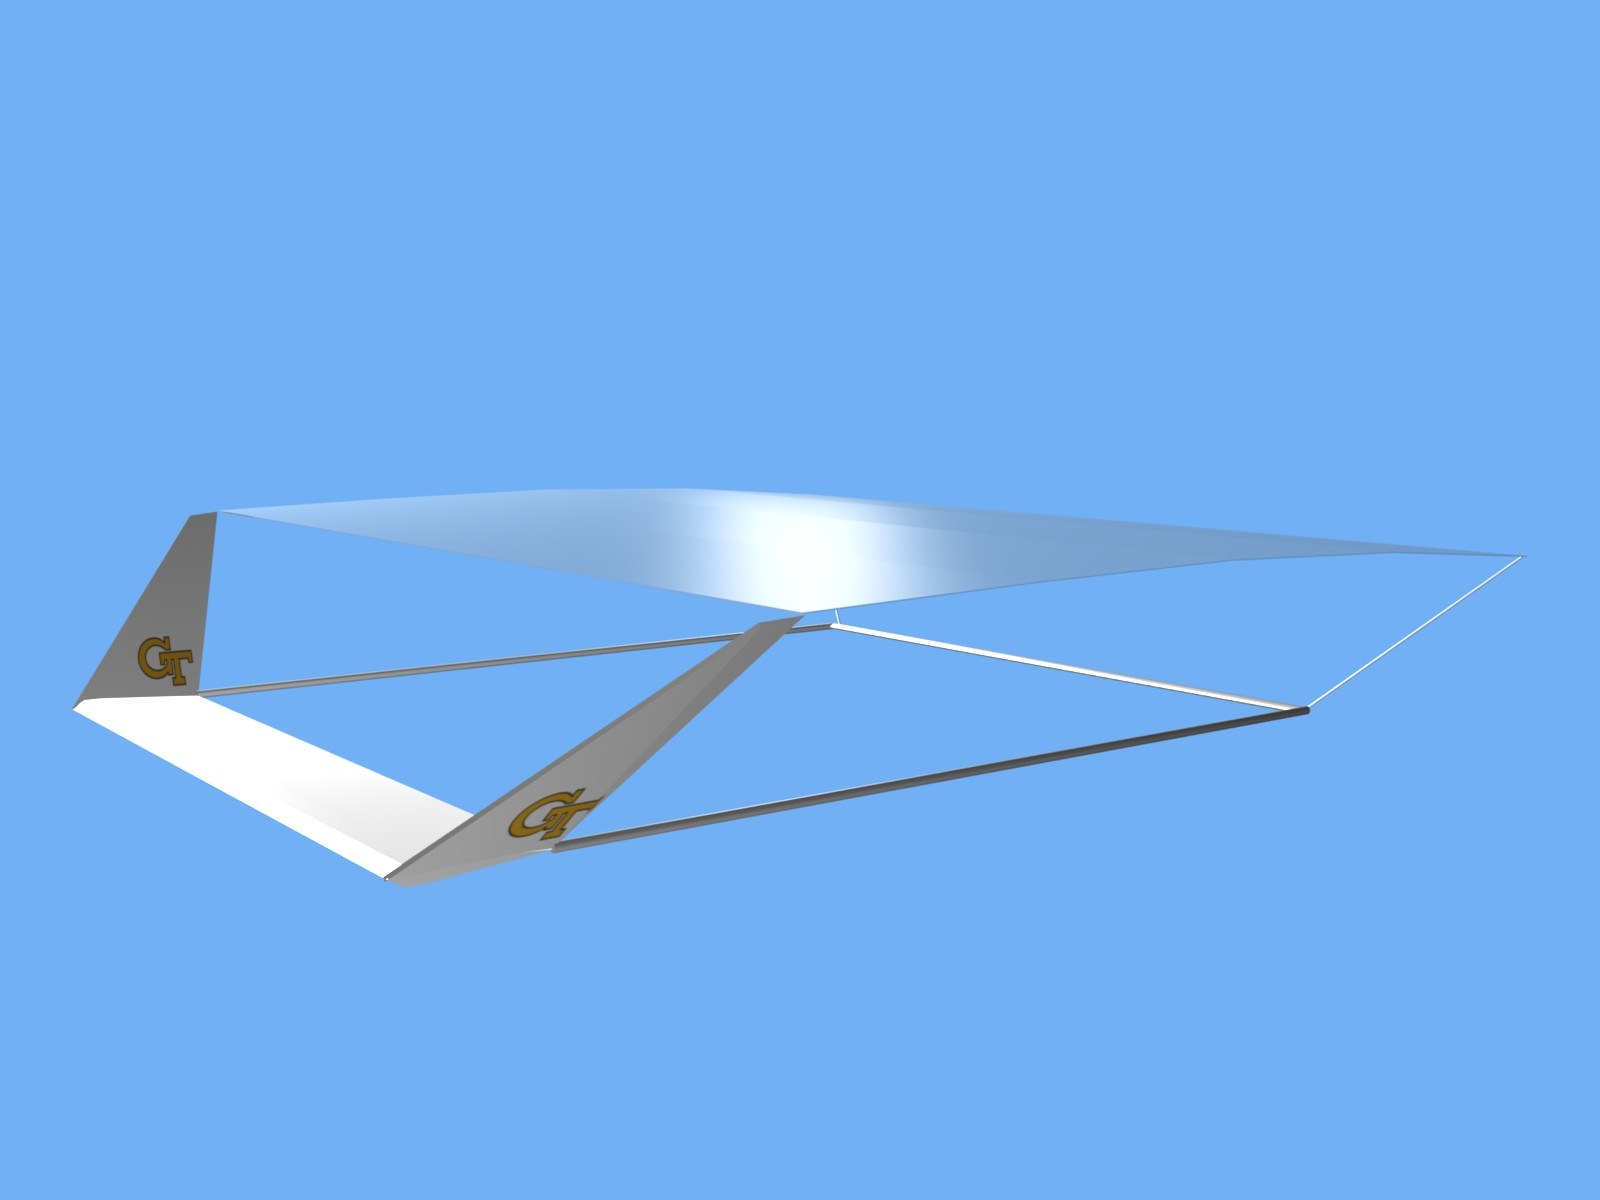
\includegraphics[width = 0.7\linewidth]{FlyingCarpet.jpg}
\centering
\caption{An artist's concept of the Flying Leaf}
\label{flyingLeaf}
\end{figure}

\section{Project Scope}
This semester's project aims to develop the Flying Leaf Concept, specifically its aerodynamics. During a 12-hour night, the Flying Leaf must start
at its cruising altitude of 100,000 feet and descend no lower than 60,000 feet, the upper limit of controlled airspace. In order to achieve
that, it must descend at an rate no greater than 0.282 m/s. This requires that the lift be sufficiently high, to minimize the airspeed required,
and the drag be sufficiently low, to minimize the glide slope. Therefore, the lift and drag propoerties of the sheet are critical to meeting
the performance requirements. The purpose of this study was to measure and if necessary improve the aerodynamics of the sheet. Ultimately,
three things were accomplished. The lift and drag required to meet the descent requirement were computed theoretically, computational predictions
for the lift and drag of the sheet were established, and method and apparatus for measuring the lift and drag of the sheet were developed.
Our experimental work was divided into two separate experiments. The first is to measure the drag of the sheet alone (the "drag experiment")
and the other is to measure the interactions between the sheet and the wing (the "interactions experiment"). The plan for the drag experiment
is to develop a house-built force balance which can support the sheet with minimal effects on the drag. By contrast, the plan for the interactions
experiment is to build a scale model of the Flying Leaf and attach it to a standard force balance, and measure its lift and drag with and without
the sheet installed.

\chapter{Define Objectives}
In order of importance:

\begin{enumerate}

\item Primary Objective: Verify that the current Flying Leaf design meets the night-time glide requirement, insofar as its lift and
drag are concerned.

	Secondary Objectives:
	\begin{itemize}
	\item Calculate lift and drag values which will meet the requirements
	\item Measure the zero-lift drag of a $20 in \times 40 in$ sheet
	\item Measure the lift-to-drag ratio at small angle of attack
	\item If either of the above results are unfavorable, devise a way to improve the sheet
	\item Test the improved sheet
	\end{itemize}

\item Primary Objective: Investigate the interactions of the wing with the sheet
	
	Secondary Objectives:
	\begin{itemize}
	\item Predict the effects of wing-sheet interactions via vortex lattice theory
	\item validate the predictions in the wind tunnel
	\item If the predictions disagree with experiment, develop and test a hypothesis to explain the discrepancy
	\item If the interactions are unfavorable, propose modifications to the Flying Leaf design to accomodate them.
	\end{itemize}

\end{enumerate}

\chapter{Prior Work}
The Flying Leaf version of the Glitter
Belt Concept has been shown to be a cost-effective, safe, and reversible alternative to other schemes of reducing
climate change. \cite{tradeoff} estimates the cost of the Glitter Belt project to be around 1.75 Trillion USD, and
\cite{flyingCarpet} concludes that the cost of the Flying Leaf version should be less than 990 Billion USD. Either
of these costs seem to be possible if redicing climate change is made a priority by developed nations. \cite{flyingCarpet}
lays out the concept which we are investigating.
During Spring 2018, \cite{us} layed more groundwork for this project by investigating the flag instability of a mylar sheet
generating lift. The following methods of reducing flag flutter were discovered.

\begin{enumerate}

\item Produce the sheet with concave edges and attach elastic material under tension to its corners (Figure \ref{corners}).
This method is easy to construct and produces positive results, but is less effective than the following two.

\item Produce the sheet with concavely parabolic edges and attach a thread under tension to its leading and trailing
edges by means of smaller transverse threads (Figure \ref{threads}). This is based upon a theory that producing uniform
longitudinal stress in the sheet is the most efficient means to reduce flutter.

\item Use adhesive to attach the sheet strongly to the support structure along it's lateral edges with negligible room
to move (Figure \ref{edges}). This was effective at reducing flutter, but the lack of elastic material may produce uneven
and high loads on the structure, and the structural devices required to uniformly attach the sheet to the support structure
may be expensive or heavy. Therefore, this device may pose disadvantages at scale.

\end{enumerate}

\begin{figure}
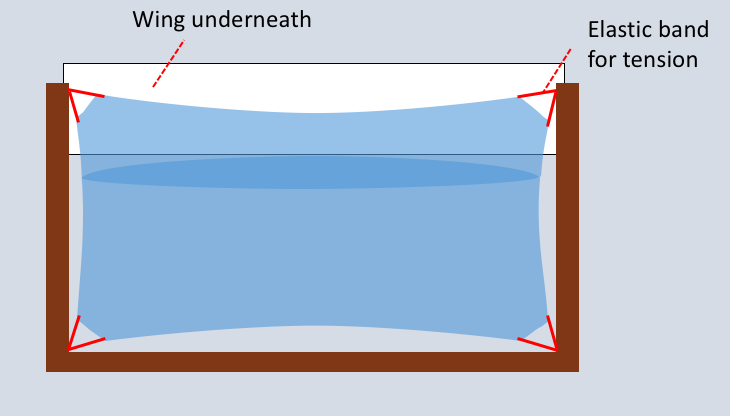
\includegraphics[width = \linewidth]{corners.png}
\caption{Reducing flutter by attaching elastic material at the corners}
\label{corners}
\end{figure}

\begin{figure}
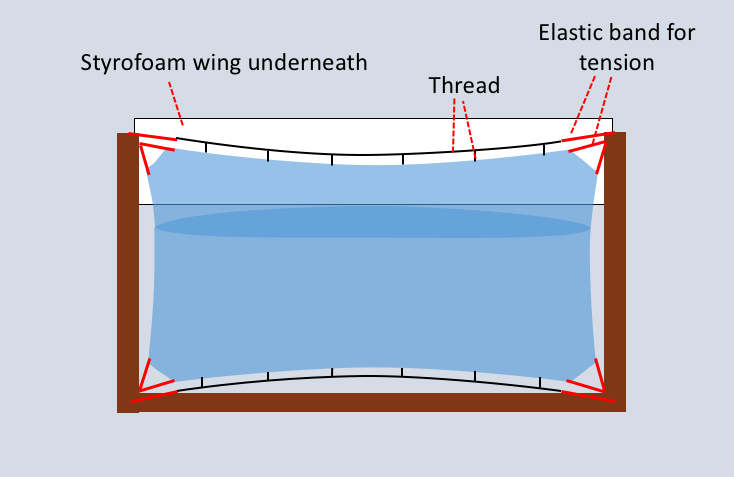
\includegraphics[width = \linewidth]{threads.png}
\caption{The preferred method of reducing flutter: parabolic threads under tension}
\label{threads}
\end{figure}

\begin{figure}
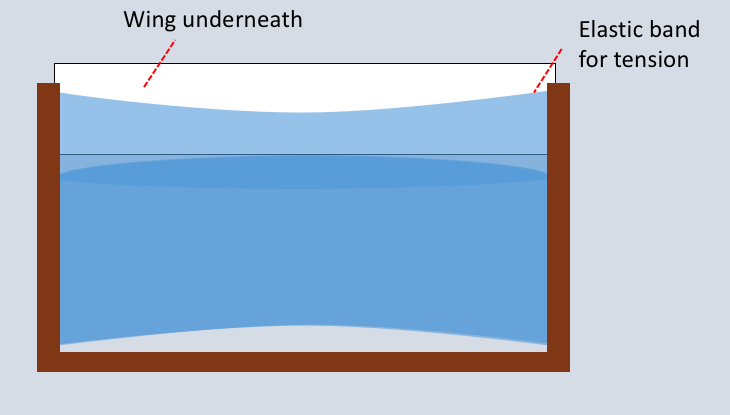
\includegraphics[width = \linewidth]{edges.png}
\caption{Reducing flutter by constraining the edges}
\label{edges}
\end{figure}

However, flutter was not eliminated entirely, so some further research into flutter reduction, both how to acheive it and how much is
required, may be warranted.

\cite{us} also measured the drag of the sheet, and found a lift-to-drag ratio which was higher than expected. However, there was some
uncertainty as to the accuracy of the measurements. So, further research is necessary to verify the drag measurements and if necessary,
find a way to reduce them.

So to summarize, prior work has shown the basic feasibility of the Flying Leaf and investigated means of reducing flutter.
 

\chapter{Project Schedule}

\begin{tabular}{|p{0.6\linewidth}|p{0.4\linewidth}|}
\hline
Task & Date Planned or Accomplished \\ \hline
Ascertain the state of the wind tunnel apparatus & 23-08-2018 \\ \hline
Review designs for a drag force balance & 27-08-2018 \\ \hline
Finish construction of the mount & 06-09-2018 \\ \hline
Introduce new members to their tasks & 07-09-2018 \\ \hline
Complete LabVIEW program to facilitate data recording & 14-09-2018 \\ \hline
Finish sheet frame & 26-09-2018 \\ \hline
Finish sheet mount structure & 03-10-2018 \\ \hline
Finalize sheet drag prediction & 09-10-2018 \\ \hline
Calculate lift and drag combinations which will meet mission requirements & 14-10-2018 \\ \hline
Ready to take drag measurements & 17-10-2018 \\ \hline
Finish drag measurements with the first iteration & 19-10-2018 \\ \hline
Finish interaction force predictions & 4-11-2018 \\ \hline
Finish calibration measurements with the second iteration & Planned: 16-11-2018 \\ \hline
\end{tabular}

\chapter{Theory}
\section{Performance Target}
It is necessary to measure and reduce drag in order that the Flying Leaf can meet its night-time glide requirement. Therefore, it should
be known what drag value must be achieved in order to meet the mission requirement. In this section, performance requirements will be
derrived from the mission requirements, to be used as a target for drag reduction.

The mission requirement for descent at night is that the aircraft must start gliding at its cruising altitude of $30000m$ at sunset,
and sink no lower than $20000m$ at sunrise 12 hours later. A relationship between lift and drag coefficient which meets this requirement
will be derived. Therefore, we must be concerned with the descent rate. For all of this analysis we assume steady flight. This is not
exactly correct, because the airspeed will vary somewhat over the course of the descent. However, since the majority of the flight
should be gliding without manuvers, and the airspeed depends only on the changing density, the acceleration should be minimal,
and steady flight a
reasonable approximation. It is well known that

\[m = \frac{C_D}{C_L}\]

where m is the distance descended per unit distance advanced (a slope, of sorts), and $C_L$ and $C_D$ are the lift and drag coefficients.
The rate of descent will then be $Vm$ where $V$ is the airspeed. If we assume that the glide angle is shallow, so that $\sqrt{C_L^2+C_D^2}$
is approximately $C_L$, then also have

\[V = \sqrt{\frac{2W}{\rho C_L S}}\]

. The Therefore, we have a formula for the descent rate, $\frac{\partial{h}}{\partial{t}}$:

\[\frac{\partial{h}}{\partial{t}} = \frac{C_D}{C_L}\sqrt{\frac{2W}{\rho C_L S}}\]

. If the solar panels, propulsion, and structure can be made extremely light, then $\frac{W}{S}$ is approximately equal to the areal
weight density of the mylar sheet (although this is very optimistic). For a 1-mil sheet, the areal mass density is about $0.035 \frac{kg}{m^2}$,
so the areal weight density is $0.343 \frac{N}{m^2}$.
However, $\rho$ varies as a function of altitude as seen in Figure
\ref{density}. Since the data is not easily described by an analytic
formula, a discretized approximation will be used to establish a relationship between the lift, drag, and time elapsed during a gliding
descent from $30000m$ to $20000m$. Density data from \cite{standardAtmosphere} was taken at $10m$ altitude intervals, and all calculations will
be done from that. The discretized approximation manifests as:

\begin{figure}
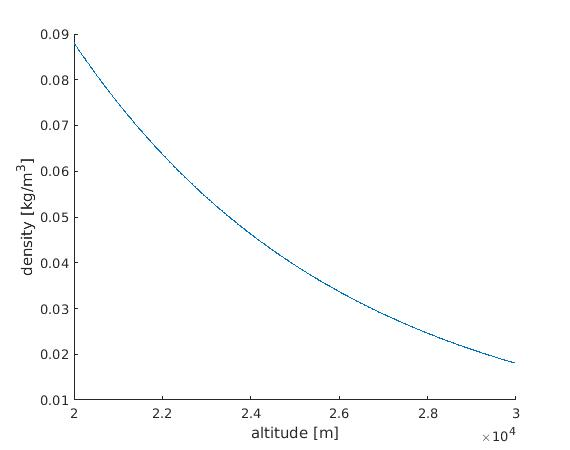
\includegraphics[width = 0.7\linewidth]{density.jpg}
\centering
\caption{Standard atmosphere data from \cite{standardAtmosphere} on flight conditions during gliding descent.}
\label{density}
\end{figure}

\[\frac{\partial{h}}{\partial{t}} = \frac{\Delta h}{\Delta t} \]
\[\Delta t =  \frac{\Delta h C_L}{C_D}\sqrt{\frac{\rho C_L S}{2W}}\]

Summing both sides over the entire dataset, we have:
\[ \sum\Delta t = t = \sum \frac{\Delta h C_L}{C_D}\sqrt{\frac{\rho C_L S}{2W}}
= \frac{\Delta h C_L}{C_D}\sqrt{\frac{C_L S}{2W}} \sum\sqrt{\rho}\]

where $t$ is the elapsed time and $\Delta h$ is the height incriment, which for this data is always $10m$. To illustrate this relationship,
The descent profile of a 1-mil Flying Leaf with a lift coefficient of 1 and a drag coefficient of 0.01 is shown in Figure \ref{descent}.
In this case the aircraft has no trouble meeting the 12-hour descent requirement.

\begin{figure}
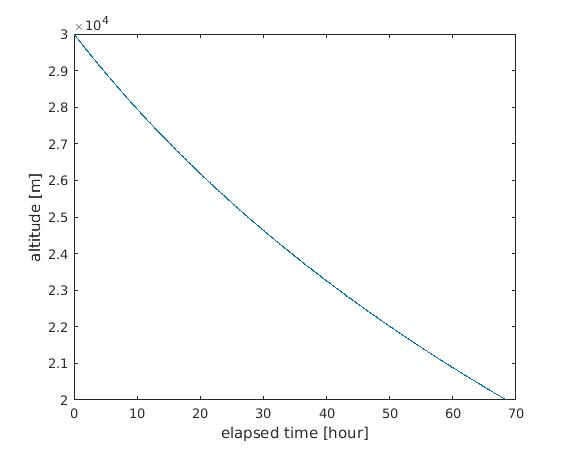
\includegraphics[width = 0.7\linewidth]{cl1cd01.jpg}
\centering
\caption{Descent profile of a 1-mil Flying Leaf aircraft with a lift coefficient of 1 and drag coefficient of 0.01.}
\label{descent}
\end{figure}

If we require that the elapsed time be greater than or equal to 12 hours, then we have derived a relationship between lift and
drag in order to meet the requirement:

\[C_D \leq \frac{\Delta h C_L}{t}\sqrt{\frac{C_L S}{2W}} \sum\sqrt{\rho}\]

Figure \ref{requirements} displays this relationship. In order for the Flying Leaf to be feasible, during our experiments we must be
able to create a sheet which, when its properties are plotted, lies above the curve.

\begin{figure}
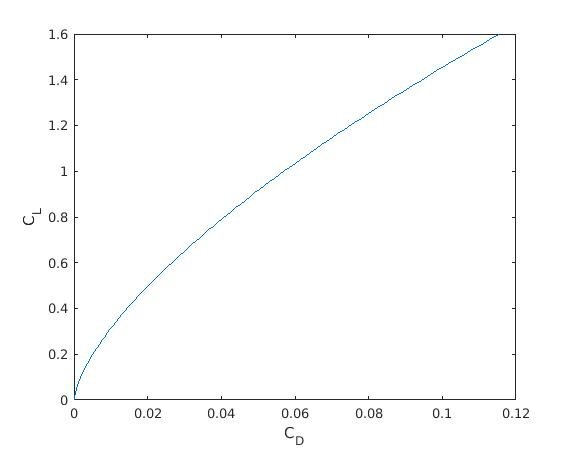
\includegraphics[width = 0.7\linewidth]{requirements.jpg}
\centering
\caption{In order to meet the 12-hour gliding descent requirement, a Flying Leaf aircraft with a 1-mil mylar sheet must be above this curve.}
\label{requirements}
\end{figure}
`
\section{Force Predictions}

\subsection{Drag Experiment}
\subsubsection{From Boundary Layer Equations}
The drag on the sheet was predicted using a standard, well tested technique based on Blasius' equation. This technique assumes laminar flow,
the accuracy of which in our wind tunnel experiments is uncertain. Based on these assumptions, the following equation from \cite{Anderson} gives
the drag on each side of the sheet.
\[ C_f = \frac{1.328}{\sqrt{Re_c}} \]
Where $C_f$ is the drag coefficient and $Re_c$ is the chord-based Reynolds number. For a $40 in \times 20 in$ sheet at $10 m/s$ in the wind
tunnel, at Atlanta's altitude, this predicts a drag of $0.141 N$, including both sides of the sheet.

\cite{Anderson} also gives the following equation for the drag in a turbulent boundary layer:
\[ C_f = \frac{0.074}{Re_c^{1/5}} \]
This predicts a drag of $0.356 N$. This formula does not take into accound the turbulence properties of the freestream. Also, it assumes
a fully turbulent boundary layer, whereas the real boundary layer of the sheet will probably be laminar in some portion and then
transition to turbulent.

Considering the respective assumptions of the laminar and turbulent calculations, we should expect our actual drag to be greater than
$0.14 N$ and less than $0.36 N$. Any value in that range should be possible to detect with a 100g load cell without overloading it.

\subsubsection{From CFD}
CFD in ANSYS Fluent was used to predict the lift and drag at nonzero angle of attack. A 2D, laminar, transient simulation was performed.
Since it is impractical to attempt to create a mesh fine enough to resolve the thickness of the sheet, a needle-like shape with sharp
leading and trailing edges was used. The maximum thickness was $1\%$ of the chord. However, in hindsight, this is too thick, and another
simulation ought to be done with a thinner sheet. In any case, it should accurately capture the phenomena at the leading and trailing edge,
although it may overpredict the drag by a small amount.

At zero angle of attack, the drag predictions match that described in the previous section with $3\%$ error. However,
at nonzero angle of attack,
the drag is remarkable high. Also, the drag polar (Fig. \ref{cfd_polar}) does
not have the shape which is expected for airfoils. In order to investigate
the cause of the drag, a the magnitude of the flow velocity near the leading edge was rendered (Fig. \ref{flat_velocity}). There appears
to be a
standing vortex near the leading edge on the downwind side of the sheet. This is probably related to the phenomenon known as ``vortex lift''
which occurs for wings with sharp leading edges.

It may be possible to avoid the vortex which is causing extra drag. Another simulation was done using a cambered sheet. The camber line
is an arc which subtends a $10\degree$ angle. This significantly improved the lift-to-drag ratio (Fig. \ref{cfd_polar}), since the sheet was
able to avoid the
leading edge vortex while simultaneously generating lift (Fig. \ref{cambered_velocity}). The lift-to-drag ratio is still not very impressive,
but this can probably be
improved by finding a more appopriate shape for the camber line.

\begin{figure}
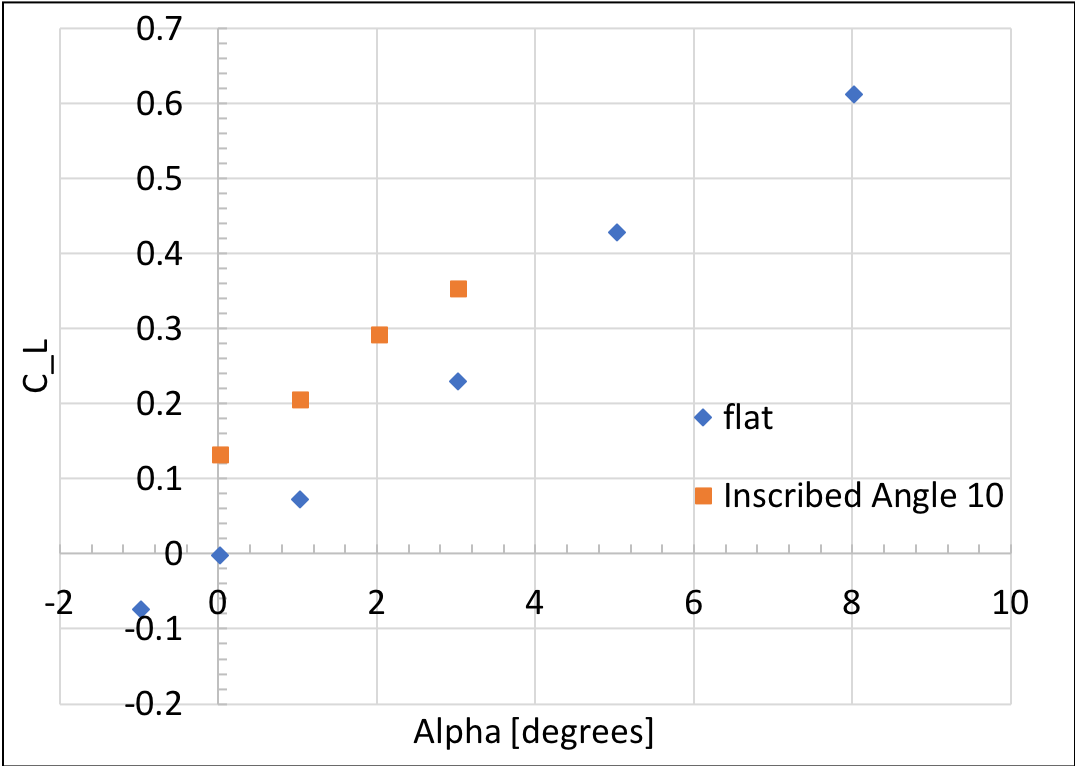
\includegraphics[width = 0.47\linewidth]{lift.png}
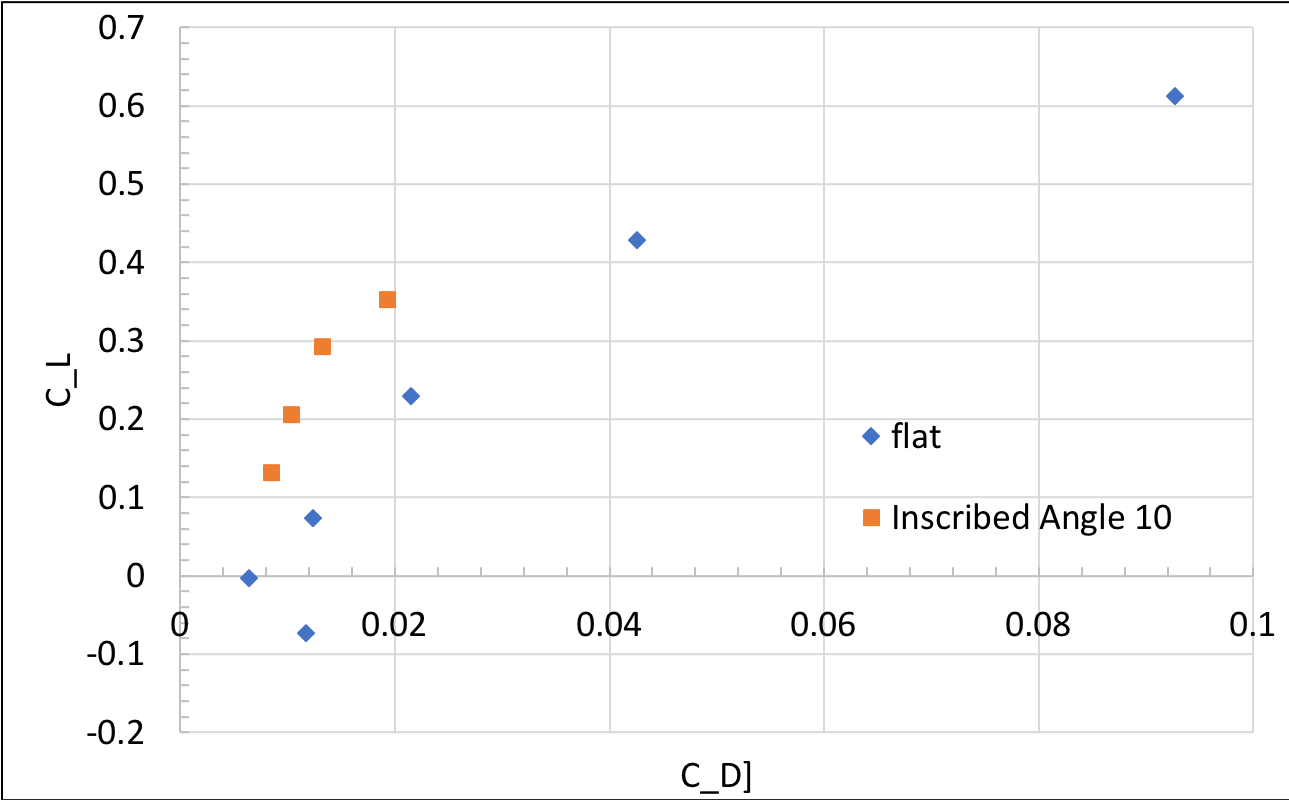
\includegraphics[width = 0.53\linewidth]{polar.png}
\caption{Lift and drag data from CFD simulations of both sheets}
\label{cfd_polar}
\end{figure}

\begin{figure}
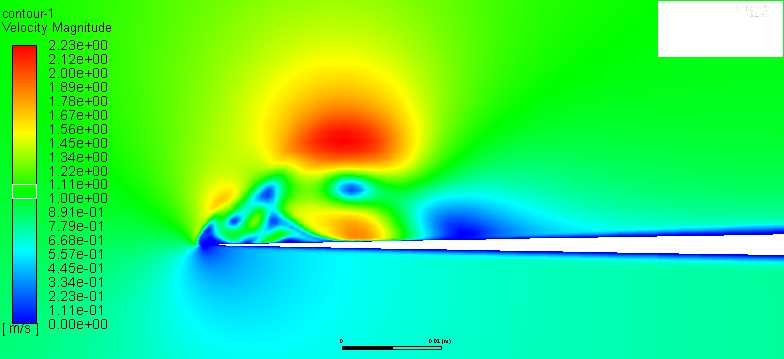
\includegraphics[width = \linewidth]{flat.jpg}
\caption{The flat sheet at $\alpha = 5\degree$}
\label{flat_velocity}
\end{figure}

\begin{figure}
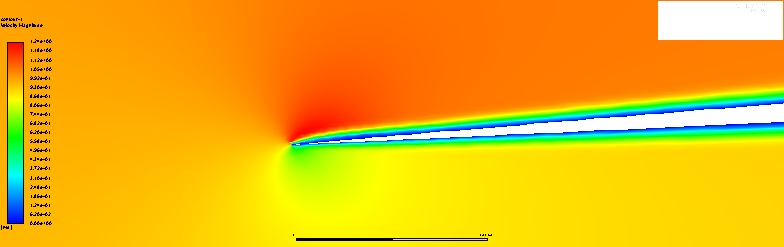
\includegraphics[width = \linewidth]{alpha2.jpg}
\caption{The cambered sheet at $\alpha = 2\degree$}
\label{cambered_velocity}
\end{figure}

From the Fluent simulation, a linear regression was calculated which relates the lift coefficint to the angle of attack. From
this regression, the lift curve slope was found to be 4.492, with the angle taken in radians. This is 0.715 times the value predicted
by potential flow theory, indicating that the lift is significantly reduced due to viscous effects, which is usually not true of
ordinary airfoils.

\subsection{Wing-Sheet Interactions Experiment}
Interactions between the wing and the sheet should not depend heavily on viscous effects. Also, neither the wing is primarily below,
and not in front of or behind the sheet, so vortex rollup should not have a large effect. Therefore, a vortex lattice model should
be able to effectively predict the aerodynamic interactions of the wing and the sheet. Athena Vortex Lattice (AVL) was used to predict
the lift of the Flying Leaf (for more information on AVL, see \cite{AVL}).

According to the Fluent predictions, the sheet has a lift curve slope of about 0.715 times that predicted by potential flow. Since AVL
is based on potential flow theory, the altered lift curve slope affects the predictions. In order to account for this difference, the
chord of the sheet was reduced by a factor of 0.715. Thus, while the nondimensional lift curve slope remains the same, the slope of
lift with respect to alpha is reduced. The simulation was conducted with and without this correction factor. Whether the experiment
agrees with the corrected lift curve slope will validate or disprove the CFD model. A drawing of the vortex lattice model can be
found in Figure \ref{avl_model}. The results of the simulation can be found in Figures \ref{10cm_corrected} - \ref{5cm_uncorrected}.
When computing the lift curve slope, the lift coefficient was normalized based on the nominal area of the sheet ($60cm \times 30cm$),
not be the sum of the wing and sheet areas, and the angle was taken in radians.

\begin{figure}
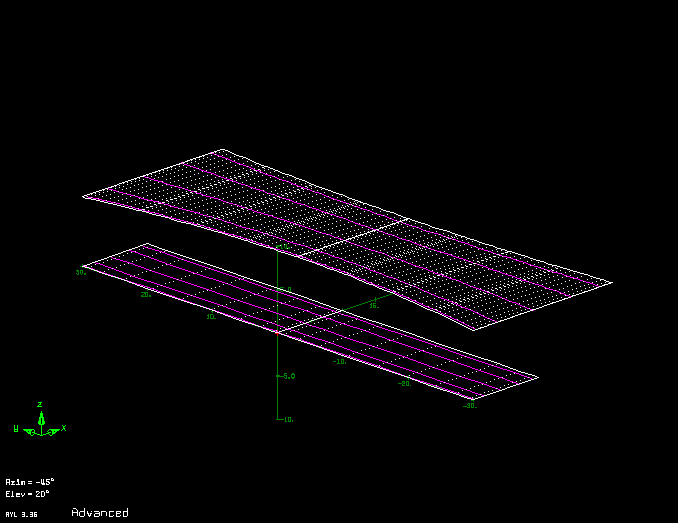
\includegraphics[width = 0.7\linewidth]{avl_model.png}
\caption{The AVL model of the wing and the sheet. The purple and dotted lines represent vortex cores.}
\label{avl_model}
\end{figure}

\begin{figure}
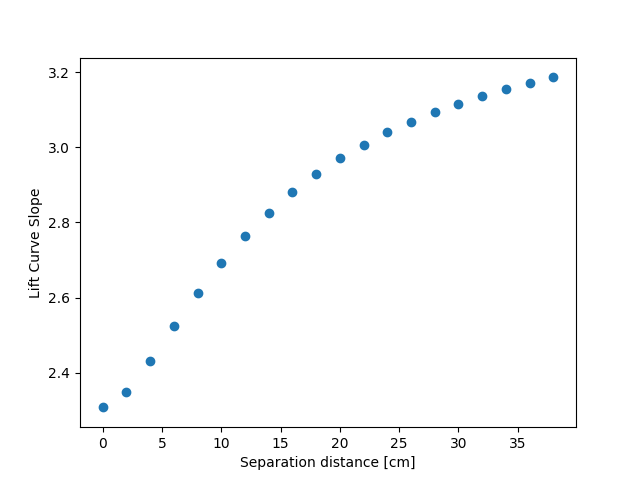
\includegraphics[width = 0.7\linewidth]{fl_chord10.png}
\caption{The results of AVL simulation with wing chord 10, with the lift curve slope correction applied.}
\label{10cm_corrected}
\end{figure}

\begin{figure}
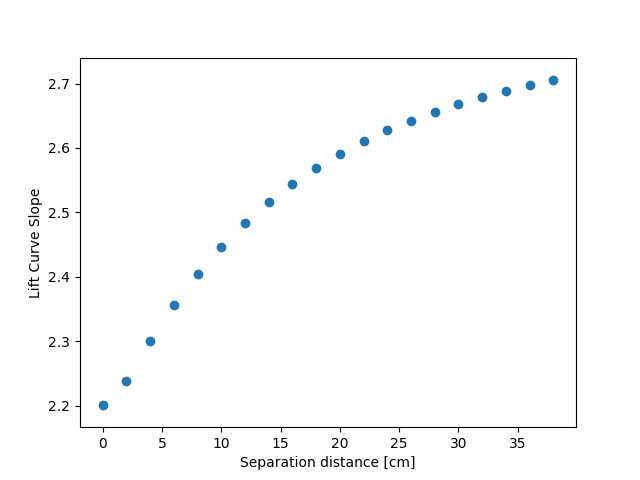
\includegraphics[width = 0.7\linewidth]{fl_chord5.png}
\caption{The results of AVL simulation with wing chord 5, with the lift curve slope correction applied.}
\label{5cm_corrected}
\end{figure}

\begin{figure}
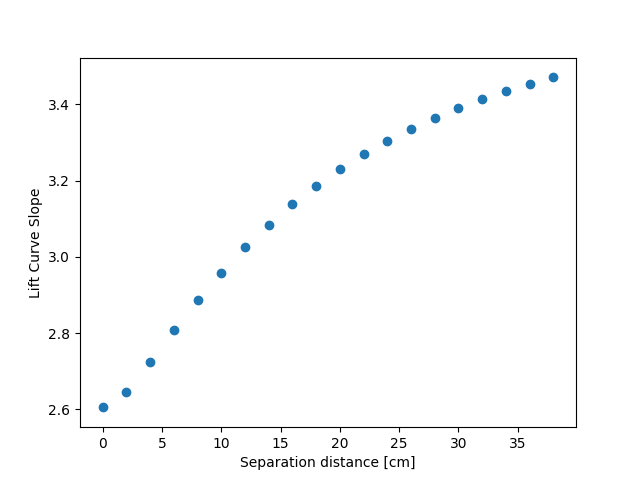
\includegraphics[width = 0.7\linewidth]{fl_chord10_cla2pi.png}
\caption{The results of AVL simulation with wing chord 10, with the lift curve slope correction not applied.}
\label{10cm_uncorrected}
\end{figure}

\begin{figure}
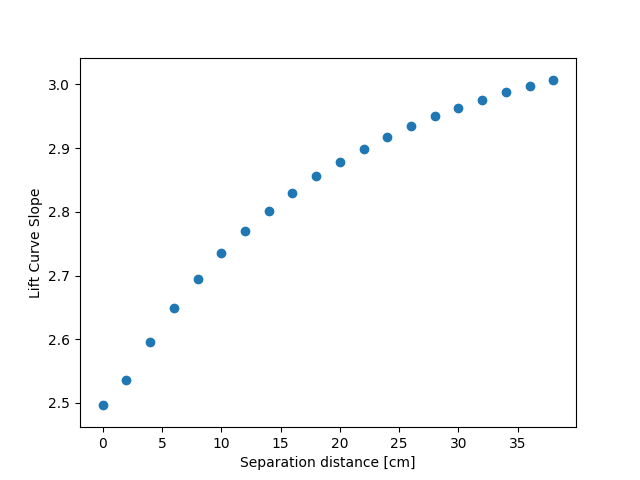
\includegraphics[width = 0.7\linewidth]{fl_chord5_cla2pi.png}
\caption{The results of AVL simulation with wing chord 5, with the lift curve slope correction not applied.}
\label{5cm_uncorrected}
\end{figure}


\chapter{Experimental Setup}

The experiments use wind tunnel tests to ascertain, and if necessary improve, the aerodynamic properties of the mylar sheet. In order to establish
a validated theory of sheet aerodynamics, we plan to take measurements of the forces on the sheet in isolation. However, since in practice the
sheet will be near a rigid wing, we are also interested in the forces on the sheet in the presence of a rigid wing. 

Therefore, we worked on two different experiments. The experment to measure the zero-lift drag of the sheet involves using
a large model in the
John Harper Wind Tunnel, and experiment on the interactions between the sheet and the wing will use the smaller wind tunnel in MK 104. Each
will use different models and force balances.

\section{Model Details}

\subsection{Drag Measurement}

\subsubsection{First Iteration}

In order to measure the zero-lift drag of the mylar sheet, a sheet which is 20 inches maximum chord by 40 inches span was used
It is suspended from a
frame via parabolic cables attached to its leading and trailing edges. So far, the frame has been constructed. It posesses a rear edge and two
lateral edges. The rear edge is made of 1/4 inch thick by 2 inch wide plywood, with styrofoam farings attached to its leading and trailing
edges to reduce drag. The lateral edges are made of 1/8 inch thick plywood which tapers from 3 inches wide at the base to 1 inch wide at the tip.

The sheet was constructed starting with a 20 by 40 inch rectangle. Then, the leading and trailing edges were cut into a parabola whose vertex
is two inches inward from the corners of the sheet. The sheet is displayed in Figure \ref{sheet_building}.

\begin{figure}
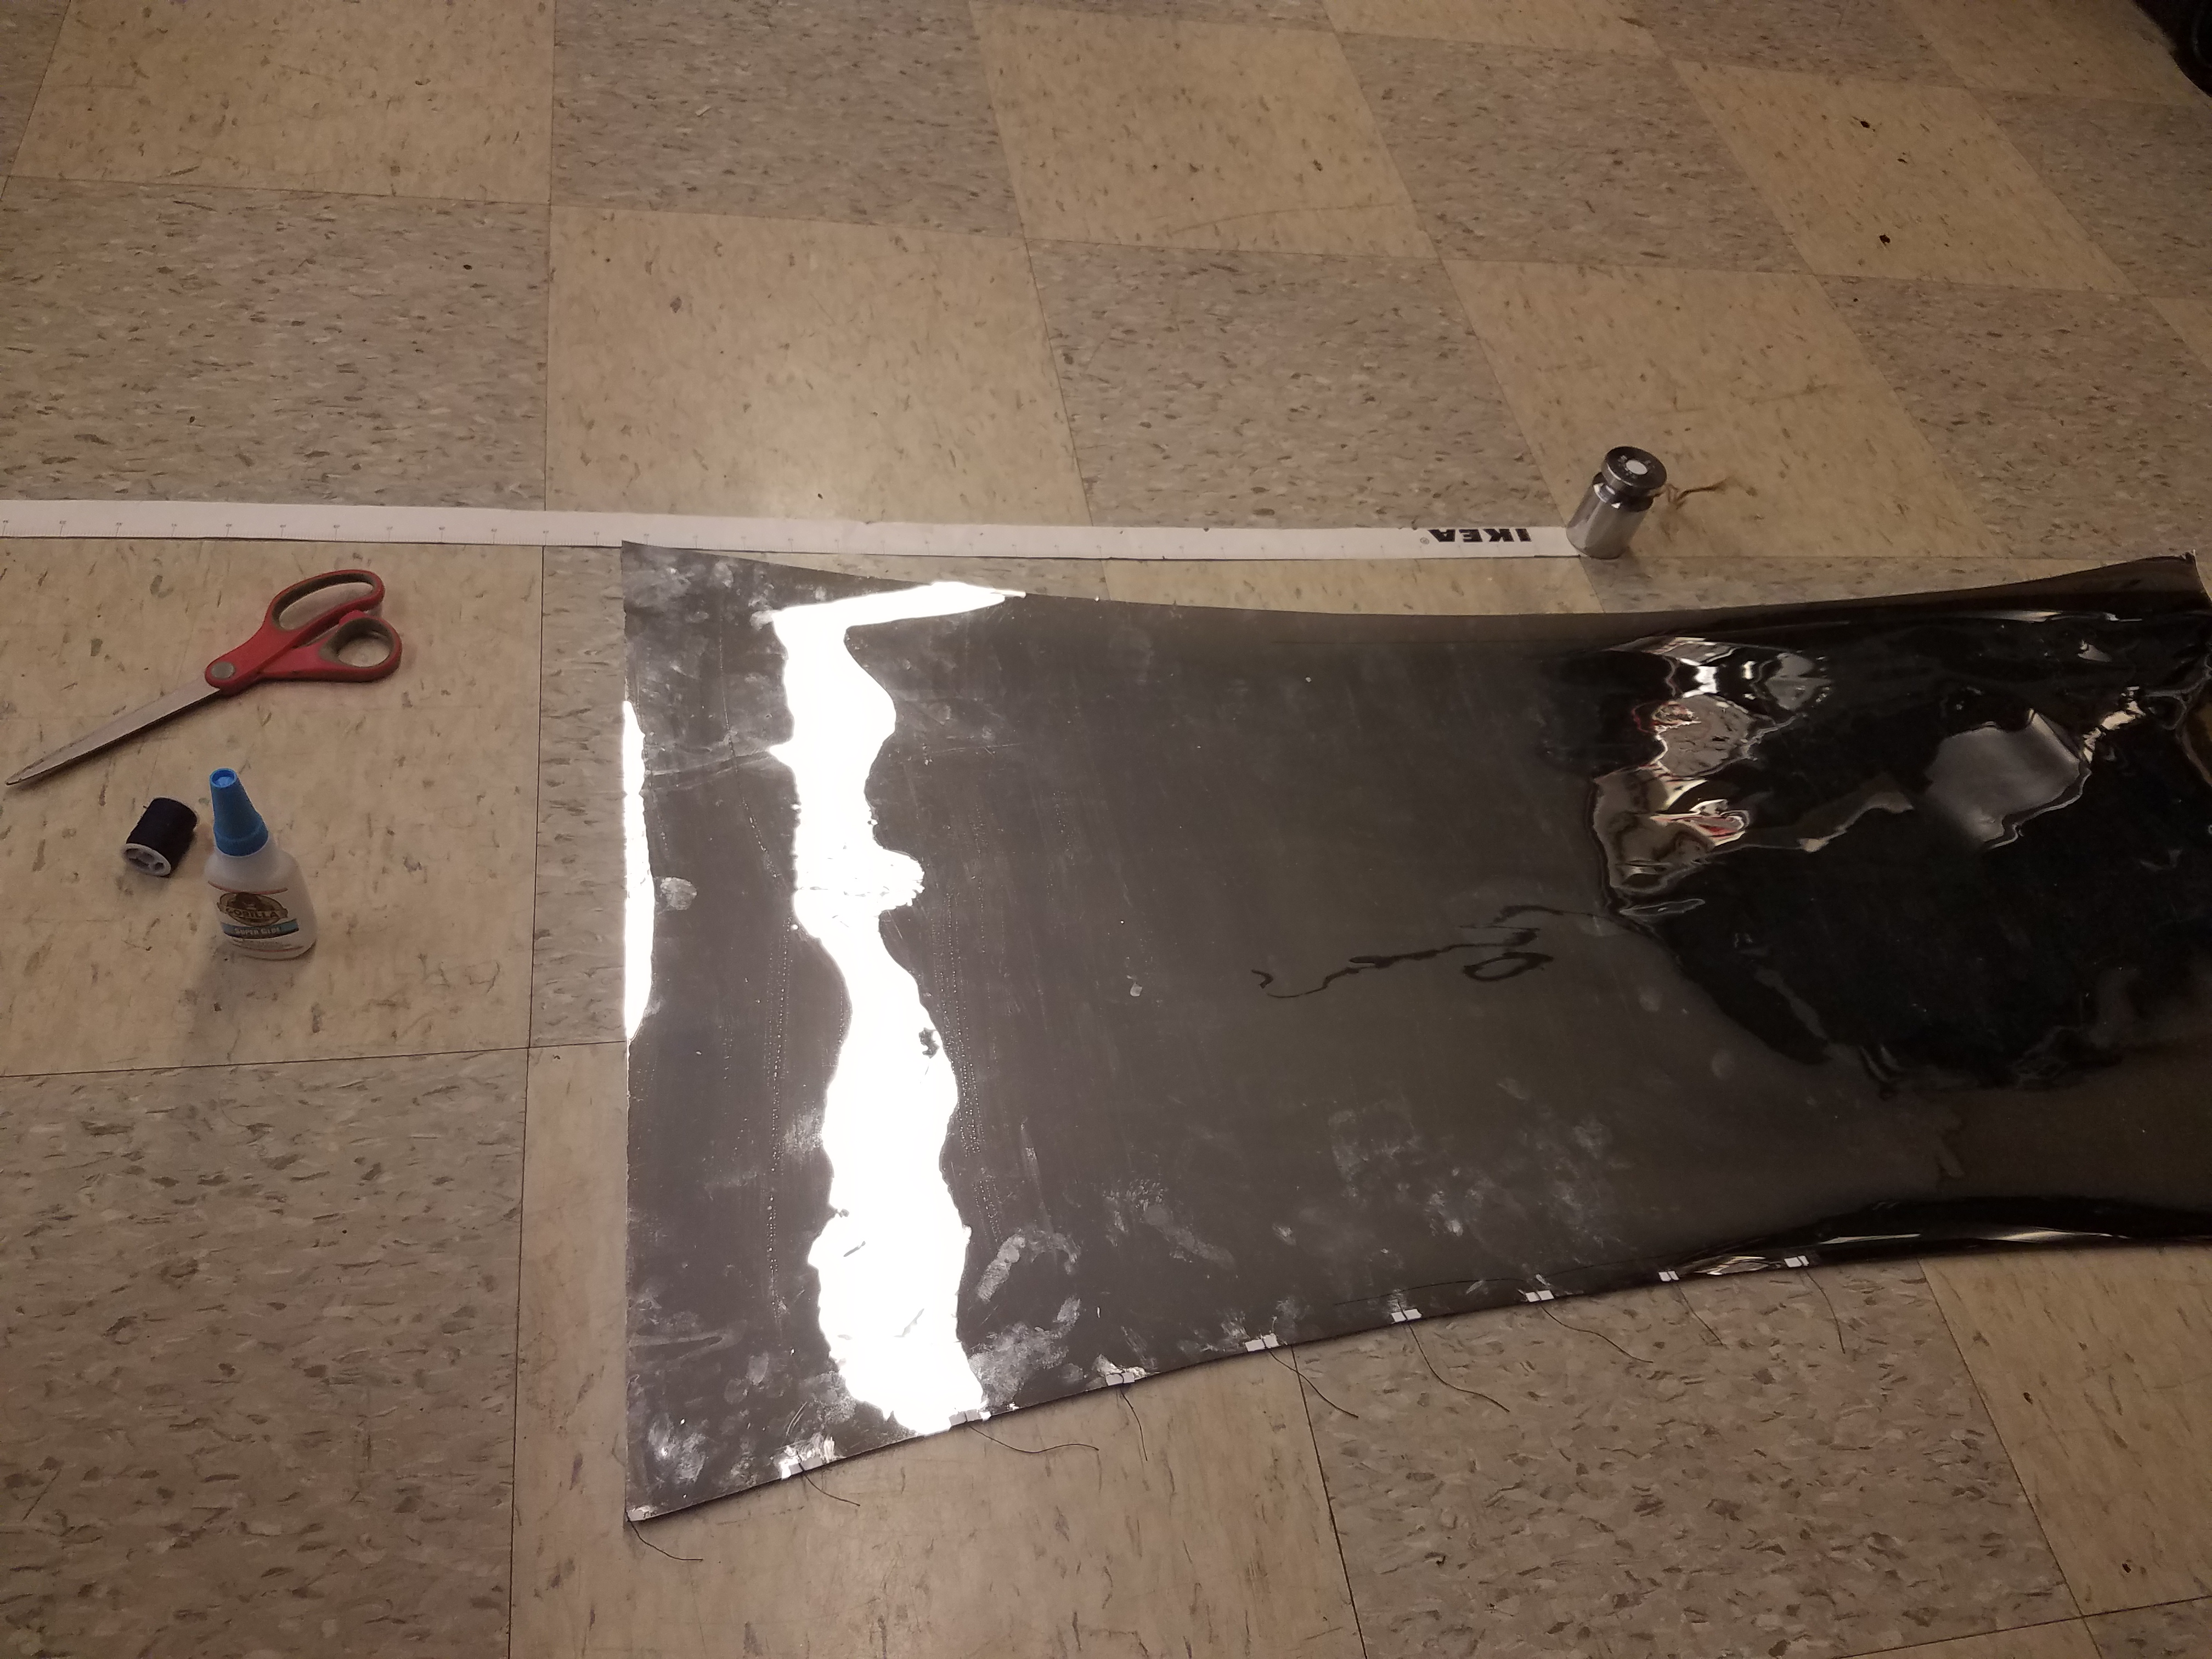
\includegraphics[width = 0.7\linewidth]{sheet_building.jpg}
\centering
\caption{Preparing the mylar sheet}
\label{sheet_building}
\end{figure}

In order to employ the flutter-reduction methods developed in \cite{us}, fishing line and thread are used in order to connect the sheet to
the frame. The fishing line runs parallel to the leading and trailing edge
and is maintained under tension by rubber bands. 30 lb-test line was used in order that the high strength should minimize any permanent deformation
due to the tension, which could have resulted in error in our experiments. The fishing line-rubber band subassembly is attached to the frame in a
fully removable way. The rubber band sits within a notch on one side of the frame, and the fishing line is wrapped through multiple revolutions
on the other side. It is important that the fishing line be removable, because of the way the drag of the frame will be measured. We are interested
in the drag of the sheet alone, without any other components. Thus, the drag measurements will first be conducted with the frame and fishing line,
without the sheet. Then, a different set of fishing lines with the sheet attached will be substituded, and the drag will be measured again, and
the drag of the frame and lines will be subtracted to obtain our final answer. Figure \ref{current} schematically illustrates the sheet and frame
assembly that will be used to take measurements.

In order to attach the sheet to the fishing line, short lengths of thread are wrapped around a small rectangle of paper (approximately 1 cm
by 3 mm), and the paper is glued to the sheet. Thus there is a significant amount of contact area for the glue to act on. Once the threads have
been installed, the sheet is positioned between the fishing lines. the lines are taped to the sheet, with about 1/4 inch separation, and then each
thread is wrapped around the fishing line several times, and a drop of superglue is applied. After the glue has dried, the tape is removed.

\begin{figure}
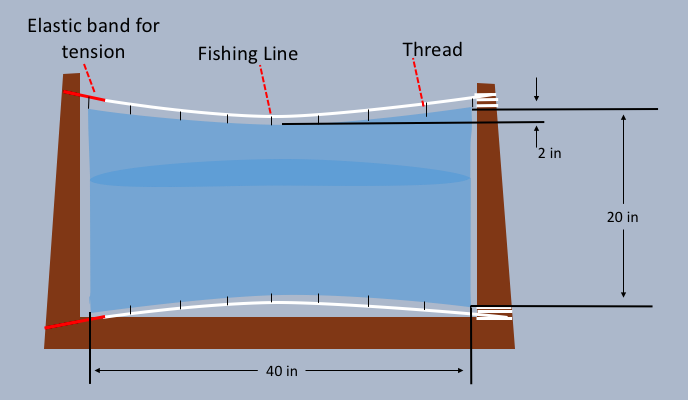
\includegraphics[width = \linewidth]{current.png}
\caption{The sheet and frame used to measure drag}
\label{current}
\end{figure}

The tension has not been precisely measured, but measures were taken to ensure that the tensions
in the leading edge- and trailing edge-fising line are equal. The amount of tension which is supplied by the rubber band is controlled by lengthening
or shortening the fishing line, causing the rubber band to contract or strech respectively. The leading edge-line was set to length, and then tied
to the trailing edge-line by a thread. This caused both lines to deflect toward one another. The length of the trailing edge-line was adjusted
until the deflection of both lines was equal, and the length of the trailing edge-line was set. Figure \ref{tension_matching} shows this process
under way.

The frame which supports the sheet (Figure \ref{frame}) is mounted on three bearings, which will allow it to roll,
which is part of the drag measurement scheme (see
``Load Cell Details''). These bearings are attached at the middle of the rear member of the frame, and on each of the side members, 15 inches
forward of the rear.

\begin{figure}
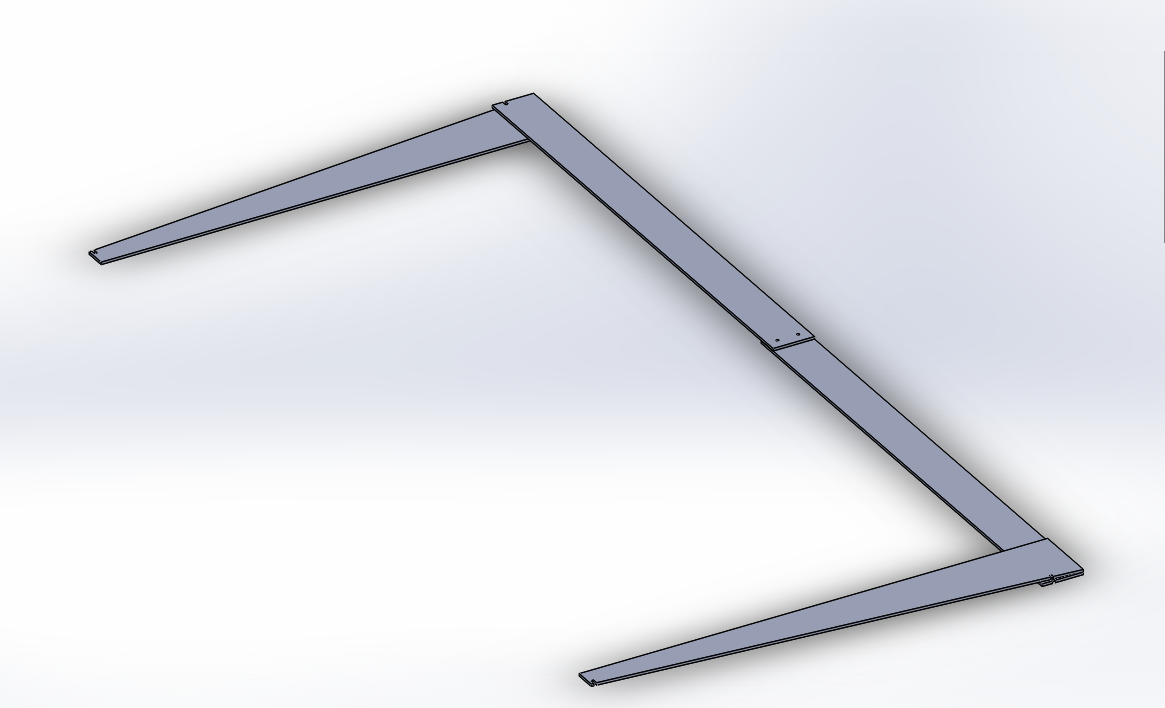
\includegraphics[width = 0.7\linewidth]{frame.png}
\centering
\caption{CAD model of the frame that holds the sheet}
\label{frame}
\end{figure}

\begin{figure}
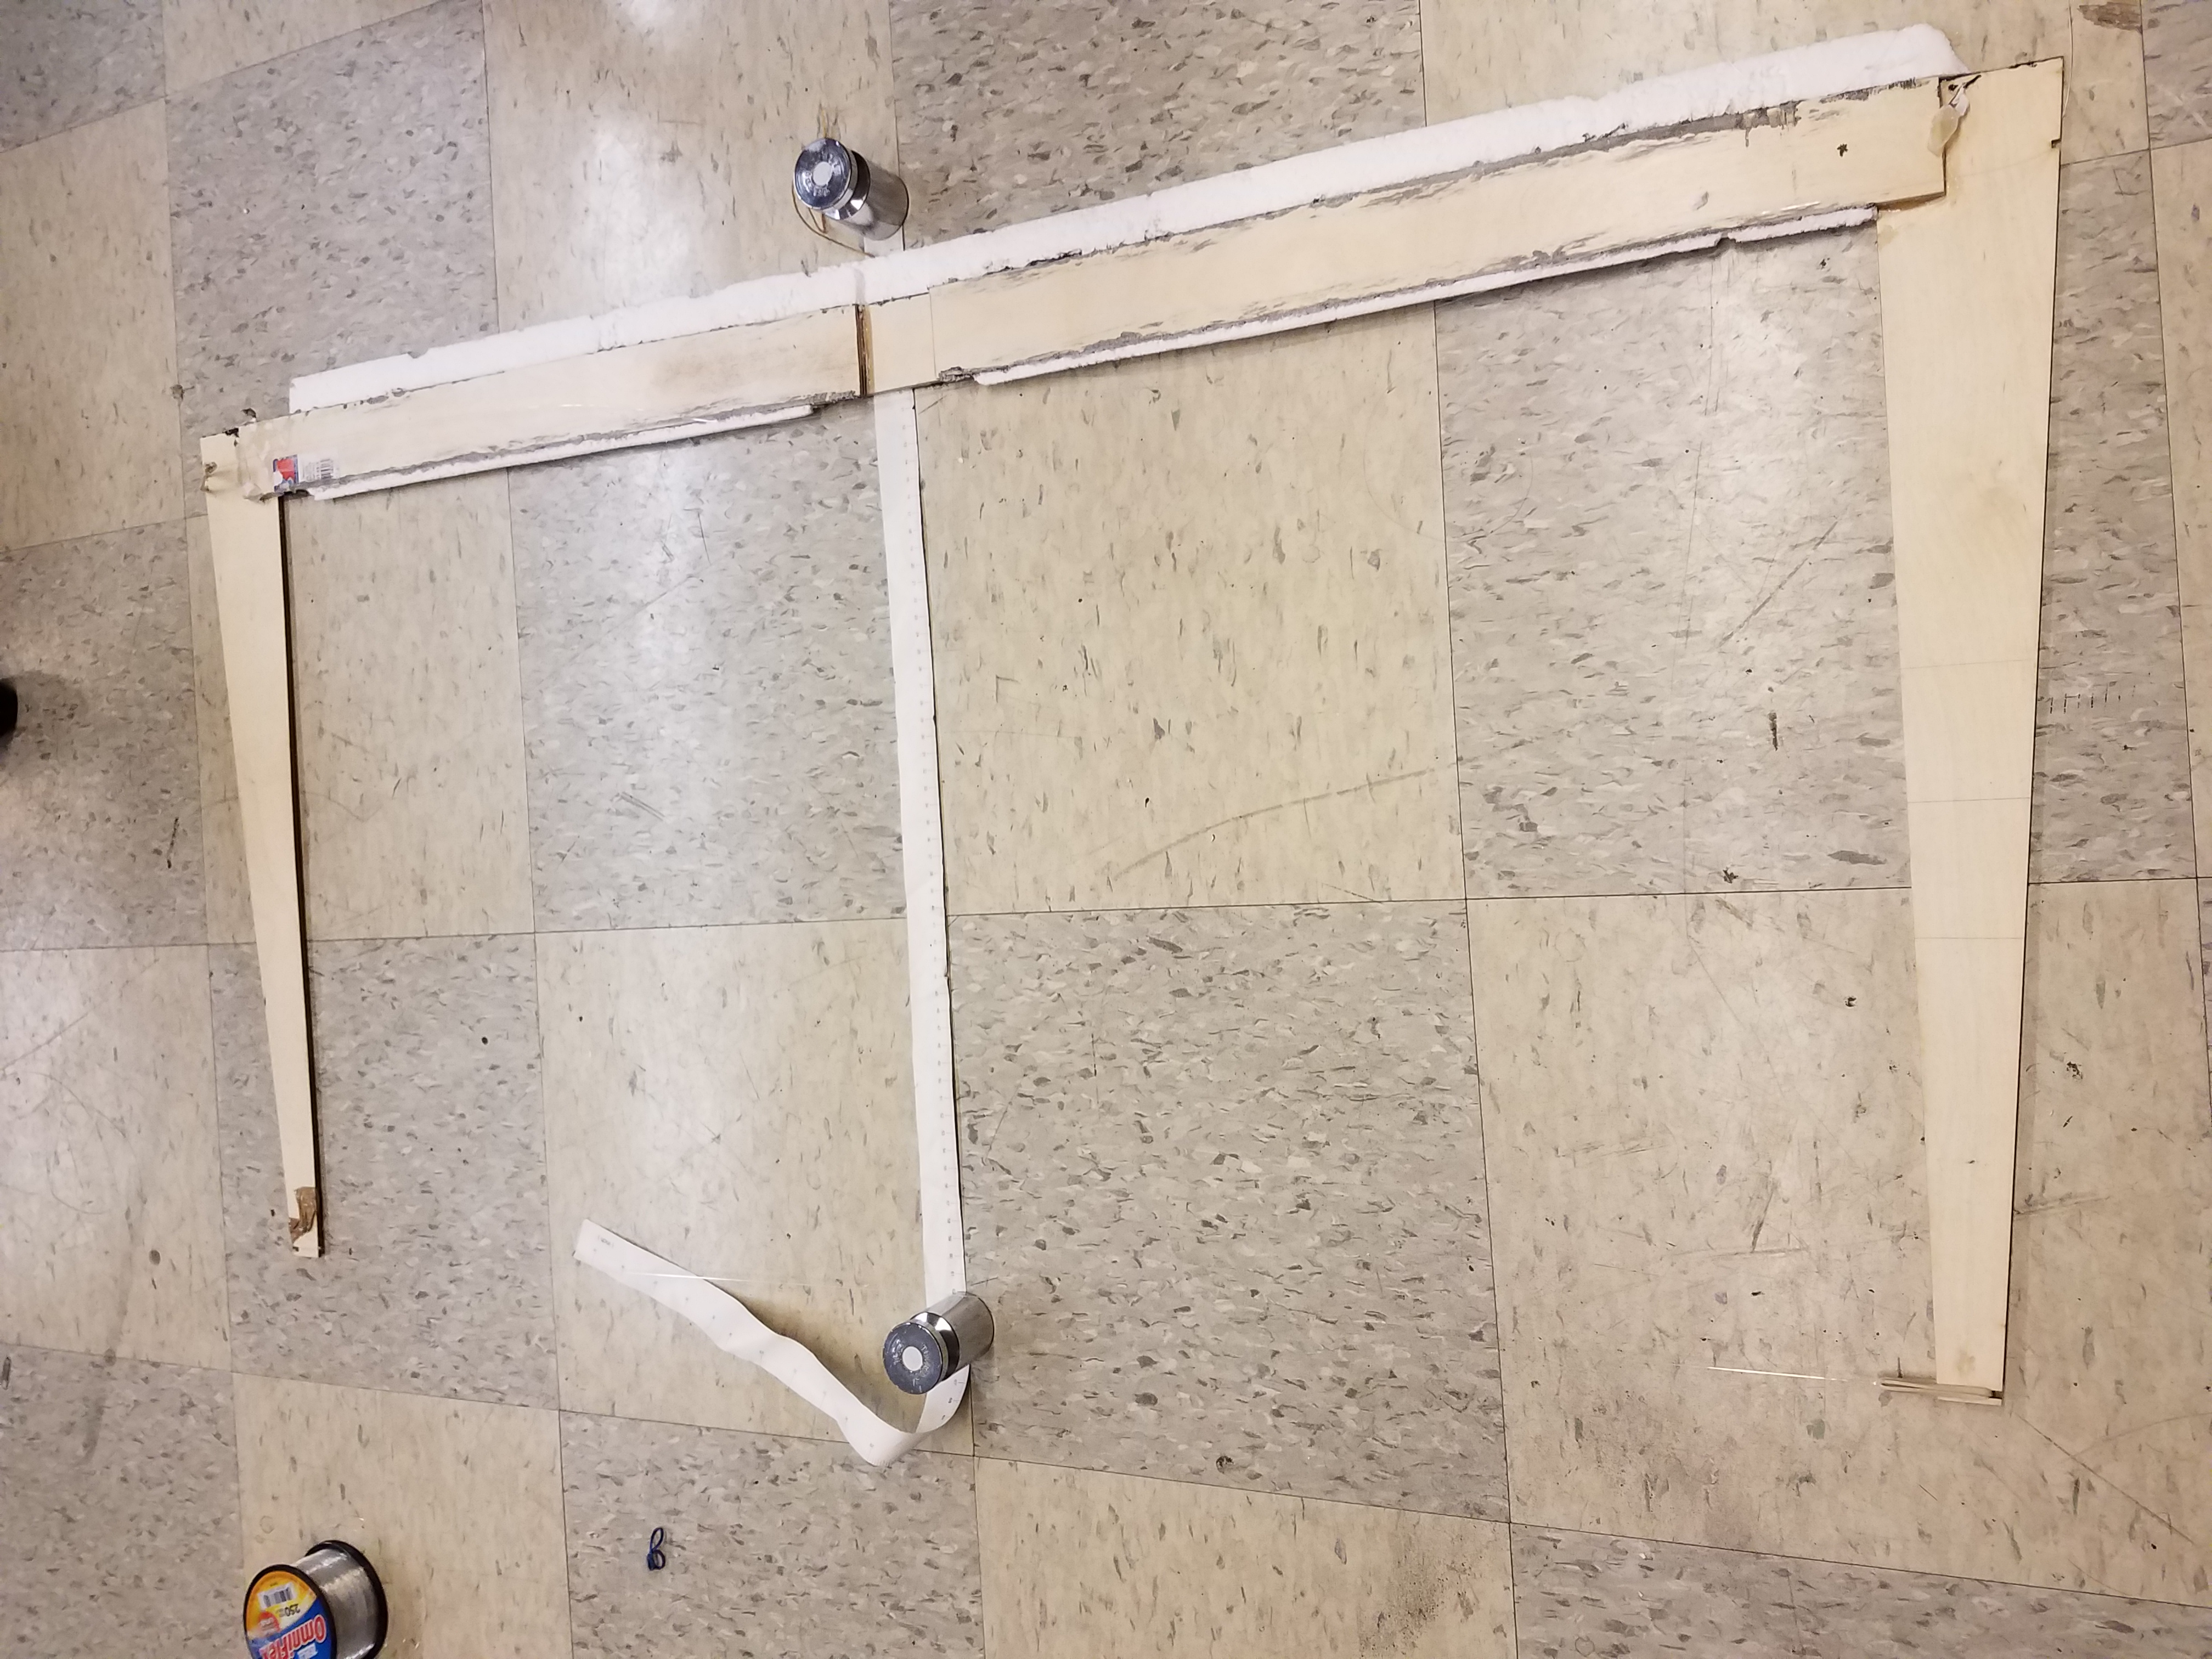
\includegraphics[width = 0.7\linewidth]{20x40flyingleaf.jpg}
\centering
\caption{Matching the tension in the leading edge- and trailing edge-fishing line}
\label{tension_matching}
\end{figure}

\subsubsection{Second Iteration}

The sheet of the second-iteration model is essentially the same as the first iteration, except that the dimensions changed. In fact, the
first iteration sheet would likely have been reused, except that it was accidentally damaged by members of another team. While being handled
carelessly, it was badly creased in such a way as would affect its drag. Let any future experimenters reading this report be warned to leave
mylar sheets in a safe location whenever unattended. By contrast to the sheet, the frame was significantly changed in the second iteration,
although that is described in detail under ``Load Cell Details''.

The sheet is 95 cm span by 47 cm maximum chord. These dimensions ensure that there will be 5 cm of separation between the frame and each
lateral edge of the sheet. This was judged to be a reasonable distance in order to maximize the size of the sheet (to maximize the aerodynamic
forces we are trying to measure) and minimize aerodynamic interference between the sheet and the frame.

The leading edge of the sheet is a parabola with equation:

\[ x = 5cm(1-(\frac{x-47.5cm}{47.5cm})^2) \]

Where x and y are standard aeronautical coordinates (x pointint toward the tail, and y pointing out the left wing), with the origin at the right,
leading-edge corner. In other words, the leading edge is a parabola with the vertex 5cm behind the corners. The trailing edge is its mirror image.
This is the design, but at the time of writing, it has not been tested, since all of the time has been taken up by fixing problems with the force
balance. However, it is expected to successfully reduce flutter, since it is based on \cite{us}.

\subsection{Wing-Sheet Interaction experiment}
I have offered some of my fellow udnergraduates the task of designing and building a model for this experiment.
The model is almost complete. It is made
primarily out of plywood, although the plan is to make the rigid wing out of foam. The distance between the wing and the sheet can be adjusted
via two plywood rods with holes placed at periodic intervals. A pin may be put in the appropriate hole to fix the distance.

There has been some difficulty in fabricating the wing which will be below the sheet, and as a result I have become more involved in its
manufacturing process. Originally, several NACA 0012 airfoil profiles were cut out of
plywood using a laser cutter, and more were cut out of foam by hand, and then abraded using a belt sander to match the plywood profiles.
Unfortunately, this model was far too imprecise and not rigid enough. A second attempt was made to machine a wing out of a single foam piece
using a CNC hot wire cutter, leaving a space to put a wooden spar inside for extra rigidity. However, given the density of the foam, the
wire cut away too much of the foam. This problem could probably be corrected by turning down the electric current, and thus the temperature
of the wire. However, the team ran out of time to use the machine, and meanwhile devised a strategy which would result in a more precise final
product.

10 NACA 0012 profiles with a 10cm chord were laser-cut out of plywood, as well as a spar. The plywood ribs were attached to the spar
by means of cyanoacrylate
adhesive. The spar is placed $25\%$ of the chord from the leading edge, which is approximately at the aerodynamic center. Thus the lift will
generate minimal torsional moment about the spar, minimizing any error in angle of attack due to deformation of the structure.
The ribs were originally cut with a flat jig which can be braced against the table during construction to eliminate any accidental twist
which may have appeared in the wing. The jigs were later cut off and the surface sanded smooth. The entire wing is wrapped in paper which
forms the skin.

I instructed the other team members in the method for sheet construction which I employ in the drag experiments. The finished sheet which
they built is shown in Figure \ref{secondIterationSheet}.

\begin{figure}
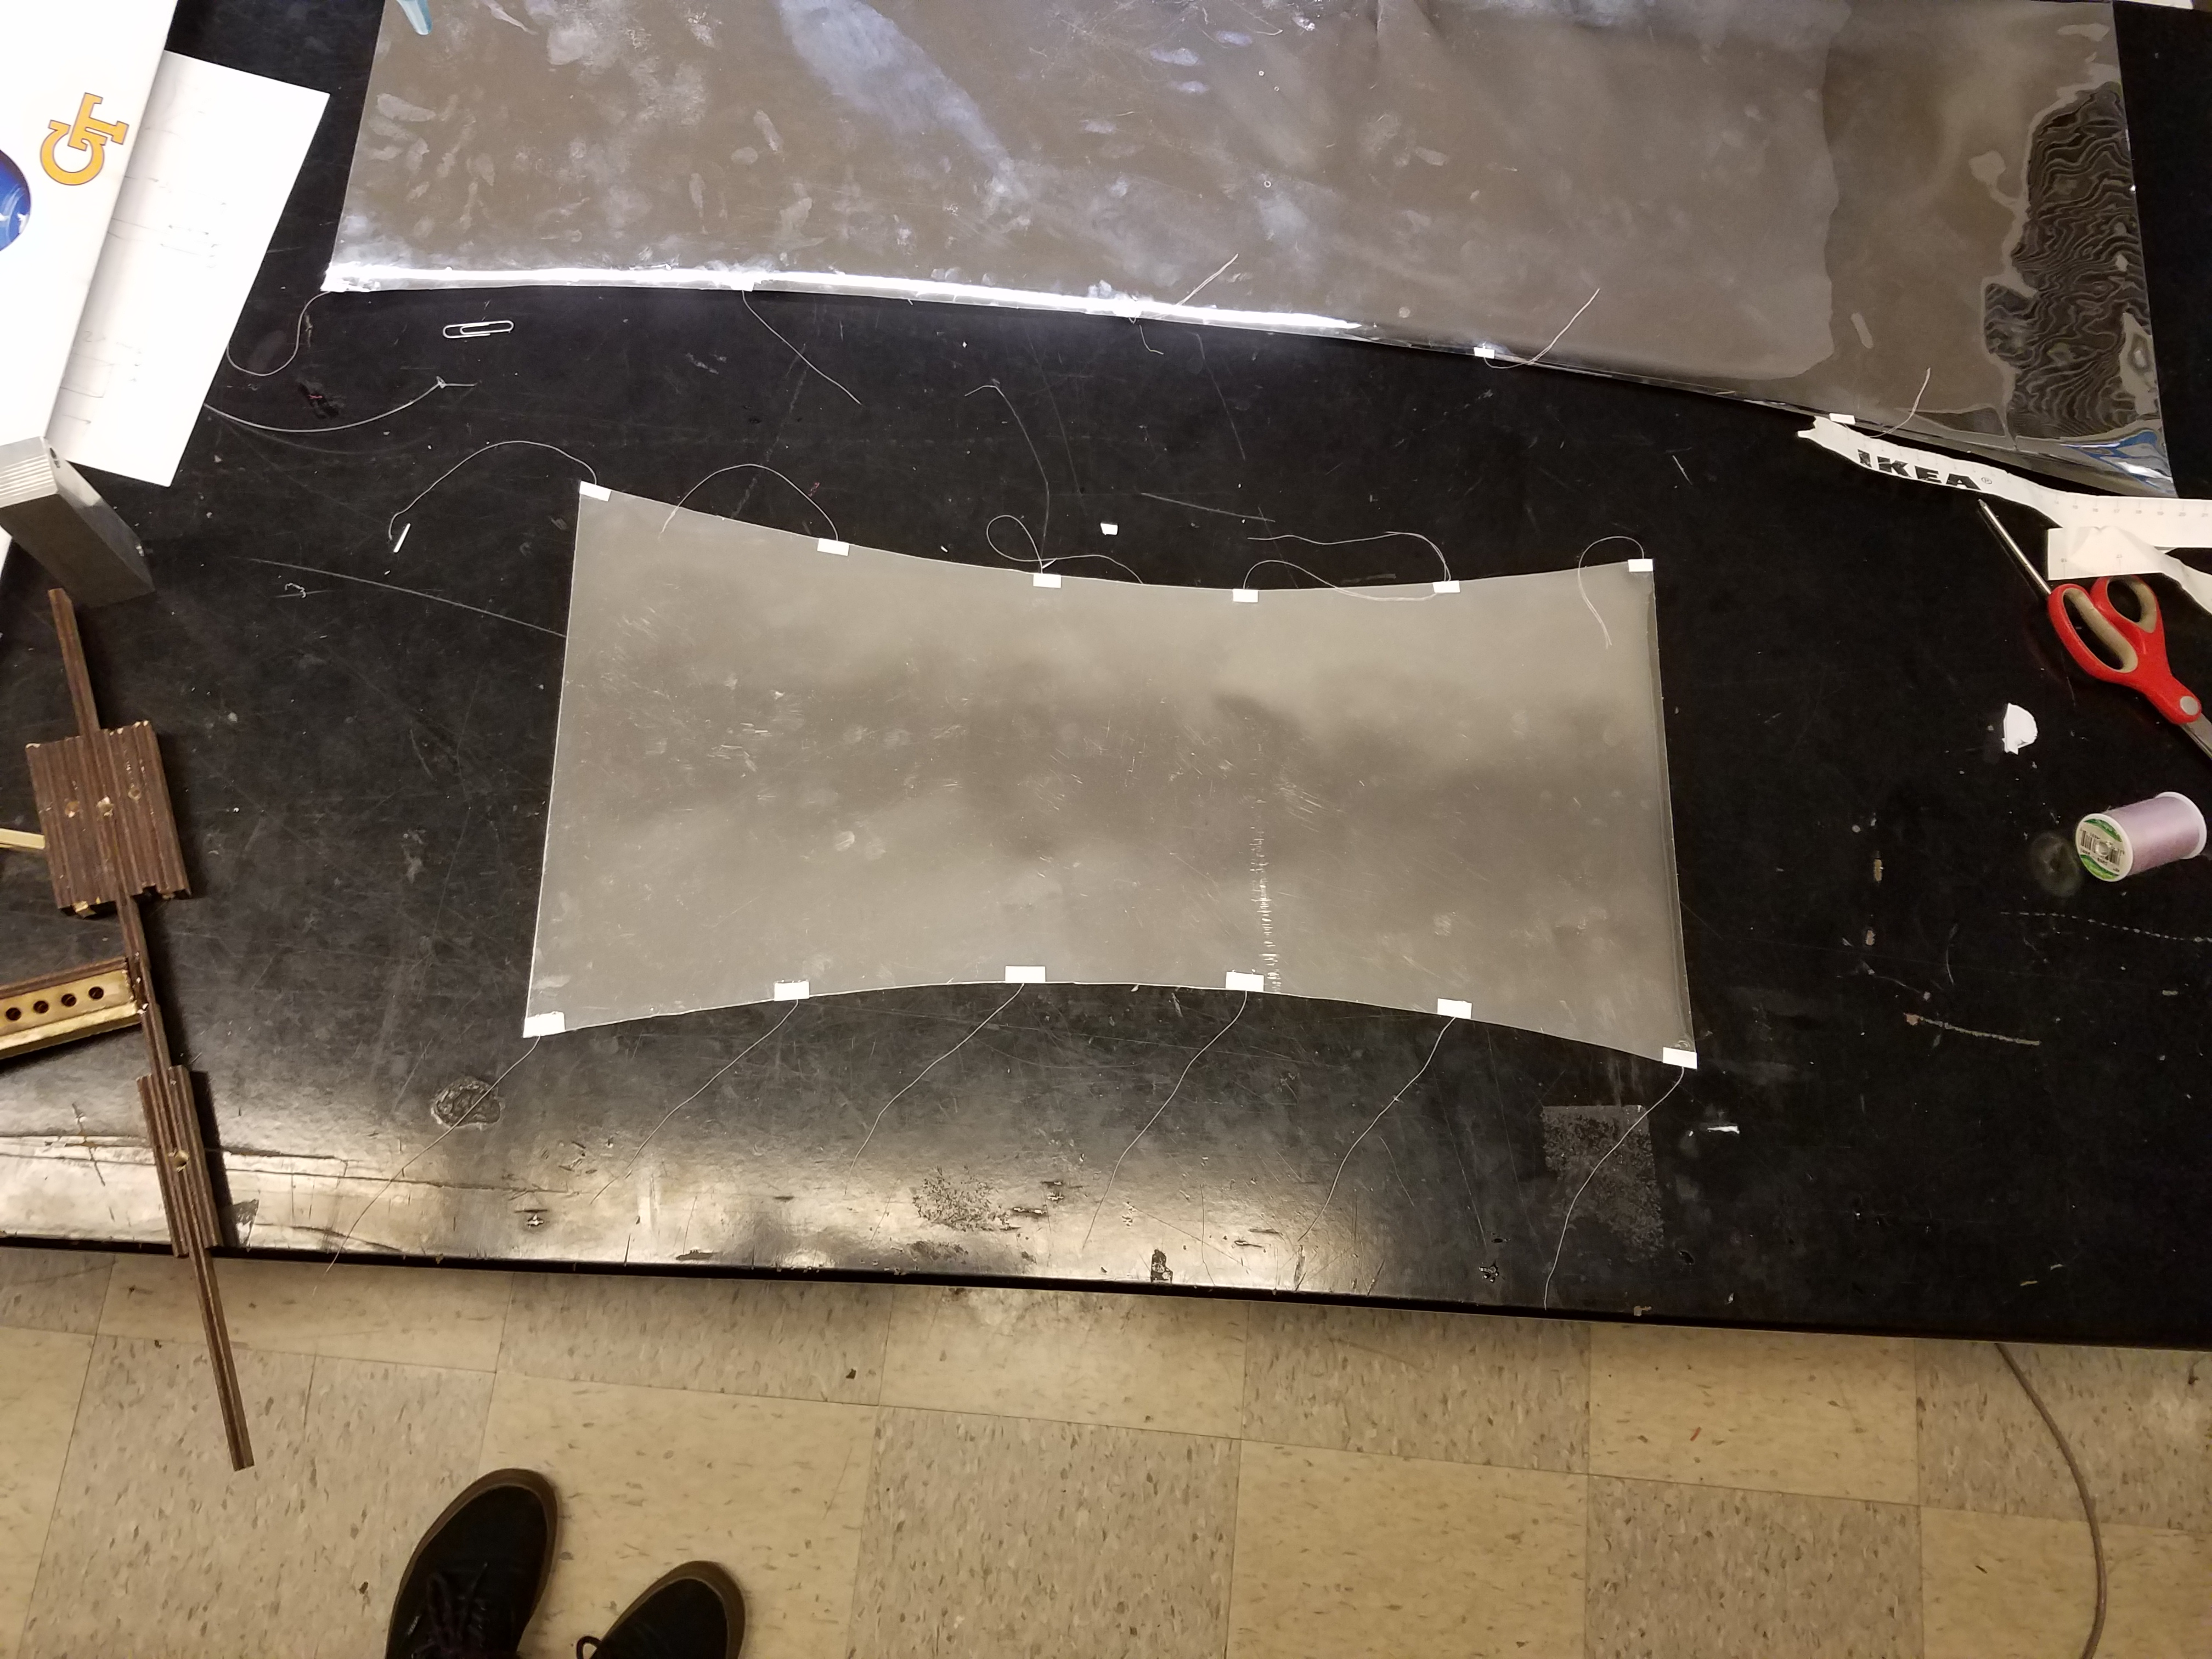
\includegraphics[width = 0.7\linewidth]{secondIterationSheet.jpg}
\centering
\caption{The sheet for the interactions experiment.}
\label{secondIterationSheet}
\end{figure}

\section{Load Cell Details}
The experimntal setup from Spring 2018 cannot be reused because the force balance is under repair away from Georgia Tech. Therefore, an alternative
force balance system must be developed. Another force balance exists, but we doubt the accuracy of its drag measurements based on previous experience.
So, we have devised two means to measure drag: An axial force balance, and a drag balance specifically designed for testing large sheets. In both
cases, force data is recorded using the same 100g load cell and data acquisition system.

\subsection{Data Acquisition}
In order to operate the load cell, a power source/filter/amplifier device is used. The output from the filter/amplifier is wired to
a NI DAQ device, which passes the signal to a LabVIEW VI. The VI was originally written by Dhwanil for the multirotor experiment,
but it has been modified to suit the purposes of this experiment.

\subsection{Load Cell Calibration}
Before any drag can be measured, the load cell must be calibrated. In other words, we read a voltage from the load cell, and we need a way to
transform that voltage into a force measurement. In order to to that, the load cell was fixed in a horizontal position, and standard weights
were hung from it. In order to verify that the load cell was sufficiently level, measurements of its angle with horizontal were taken using a
digital protractor. In each direction, it was within $1\degree$ of vertical, so that the error due to lack of levelness is certainlly less
than $0.03\%$.

Initially, problems were encountered in reading the force measurements. The data appeard to be so noisy that the changes caused by
the loads were difficult to detect. Because a digital multimeter read smooth data from the filter-amplifier, the LabVIEW program was
investigated. Ultimately, it was discovered that by changing which pins on the DAQ the filter/amplifier is plugged into solves the
problem. AIN 0 works well.

As soon as the data reading problem had been solved, standard weights were hung from the load cell. Weight ranging from 0 to 2 oz in
1/4 oz increments were hung from the load cell and data recorded for at least 20 seconds for each trial, at a sampling rate of 1k Hz.
figure \ref{data_example} shows an example of the data for one trial. Subsequently, using MATLAB, the data for each trial was averaged
and a linear regression was computed to relate the force to the numerical reading (Figure \ref{loadCellCalibration}). The slope
of this regression, which was found to be 12.9 N, is used to compute all drag measurements.

\subsection{Axial Force Balance}

For smaller models to be tested in the smaller wind tunnel, we have constructed an axial force balance.
The axial force balance uses a mechanical structure involving ball bearings
to transfer load in only one direction. The effects of moments, other components of force, and friction are minimal. It uses a 100g load cell
to measure force. The model will be attached to the axial force balance, and will rotate together with it as the angle of attack is changed.
The lift will be measured by the existing force balance, and when combined with the axial force measurements from the axial force balance,
the drag can be calculated.

There is some concern that the drag force on the axial force balance itself will interfere with measurements of the model's drag. In order to
take the drag of the balance into acount, tests will be performed on the balance without a model on it. The drag measured in these baseline tests
will be subtracted from the drag measured in model experiments. However, if the drag on the axial force balance is too high, then it may be difficult
to resolve the drag of the model. Therefore, it is advantageous to make the balance as small as possible. On the other hand, the smaller
the structure is,
the greater the load on the bearings will be (in order to balance the moment generated by the sheet's lift), and greater load will result in more
friction in the bearings. So, the structure was carefully designed to spread the load evenly among six bearings while still minimizing
the overall size.

\begin{figure}
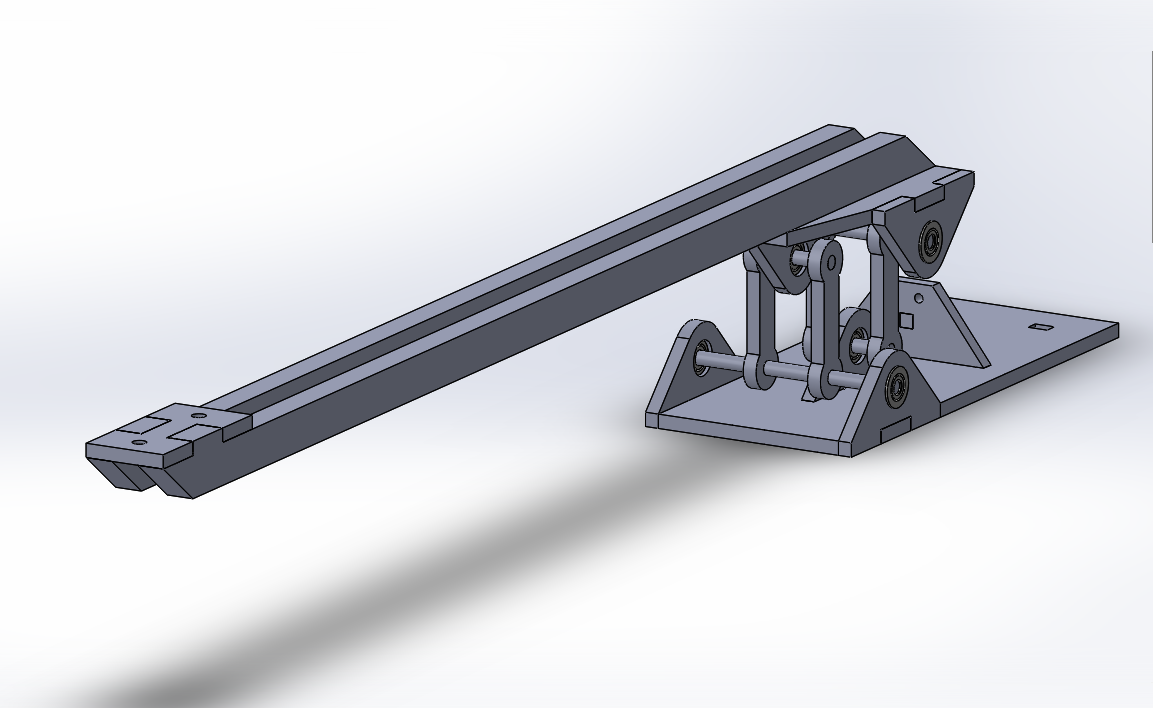
\includegraphics[width = 0.7\linewidth]{mount.png}
\centering
\caption{CAD model of axial force balance}
\label{mount}
\end{figure}


\subsection{Large Sheet Balance}

With the zero-lift drag experiment in mind, a system which will allow our 100g load cell to measure the drag of a $20 in \times
40 in$ sheet has been devised. Originally, he sheet system (described in ``Model Details'') is fitted with bearings, allowing it to roll.
The load cell is attached with screws and nuts to a laser-cut plywood assembly, and which in turn is glued to one of the rolling
surfaces. The load cell is tied to the sheet frame by a thread. Thus the sheet is constrained
from rolling in the direction of the freestream by the load cell, so the force on the load cell will be equal to the drag force
plus the friction and tilt error. The integration of the load cell into the mechanical asssembly is displayed in Figure \ref{load_cell}.

\begin{figure}
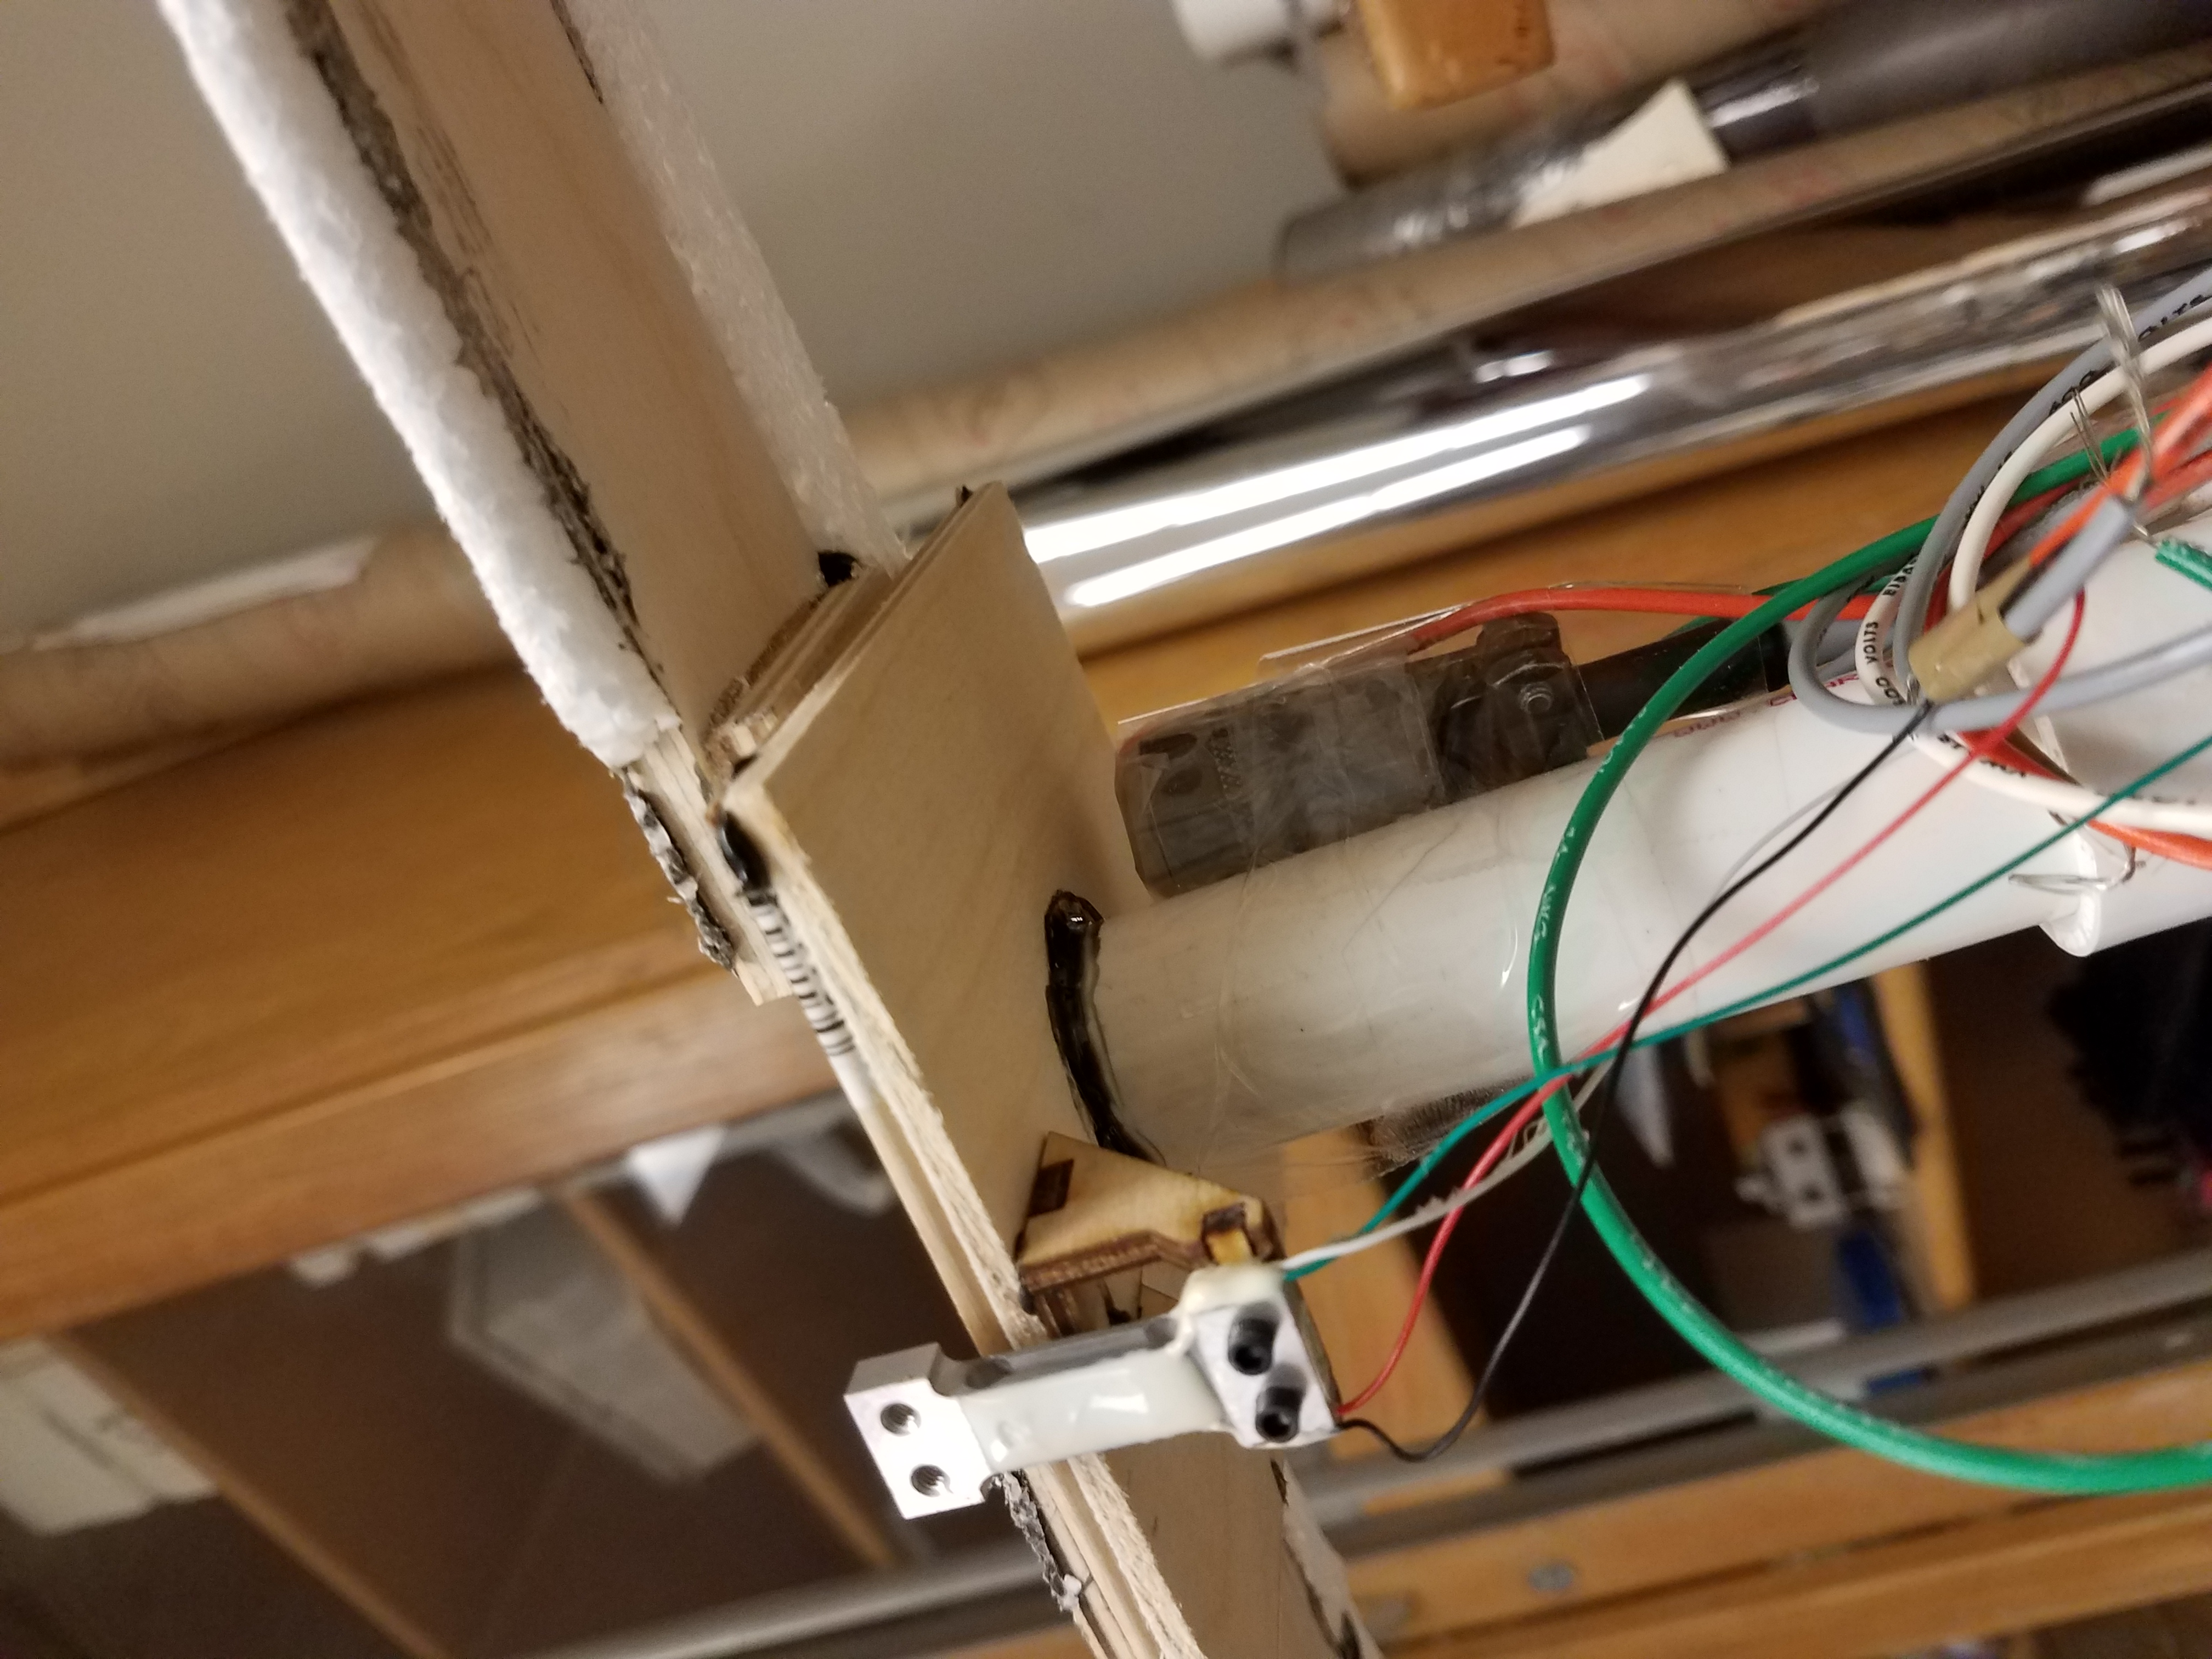
\includegraphics[angle = -90, width = 0.49\linewidth]{load_cell_insertion.jpg}
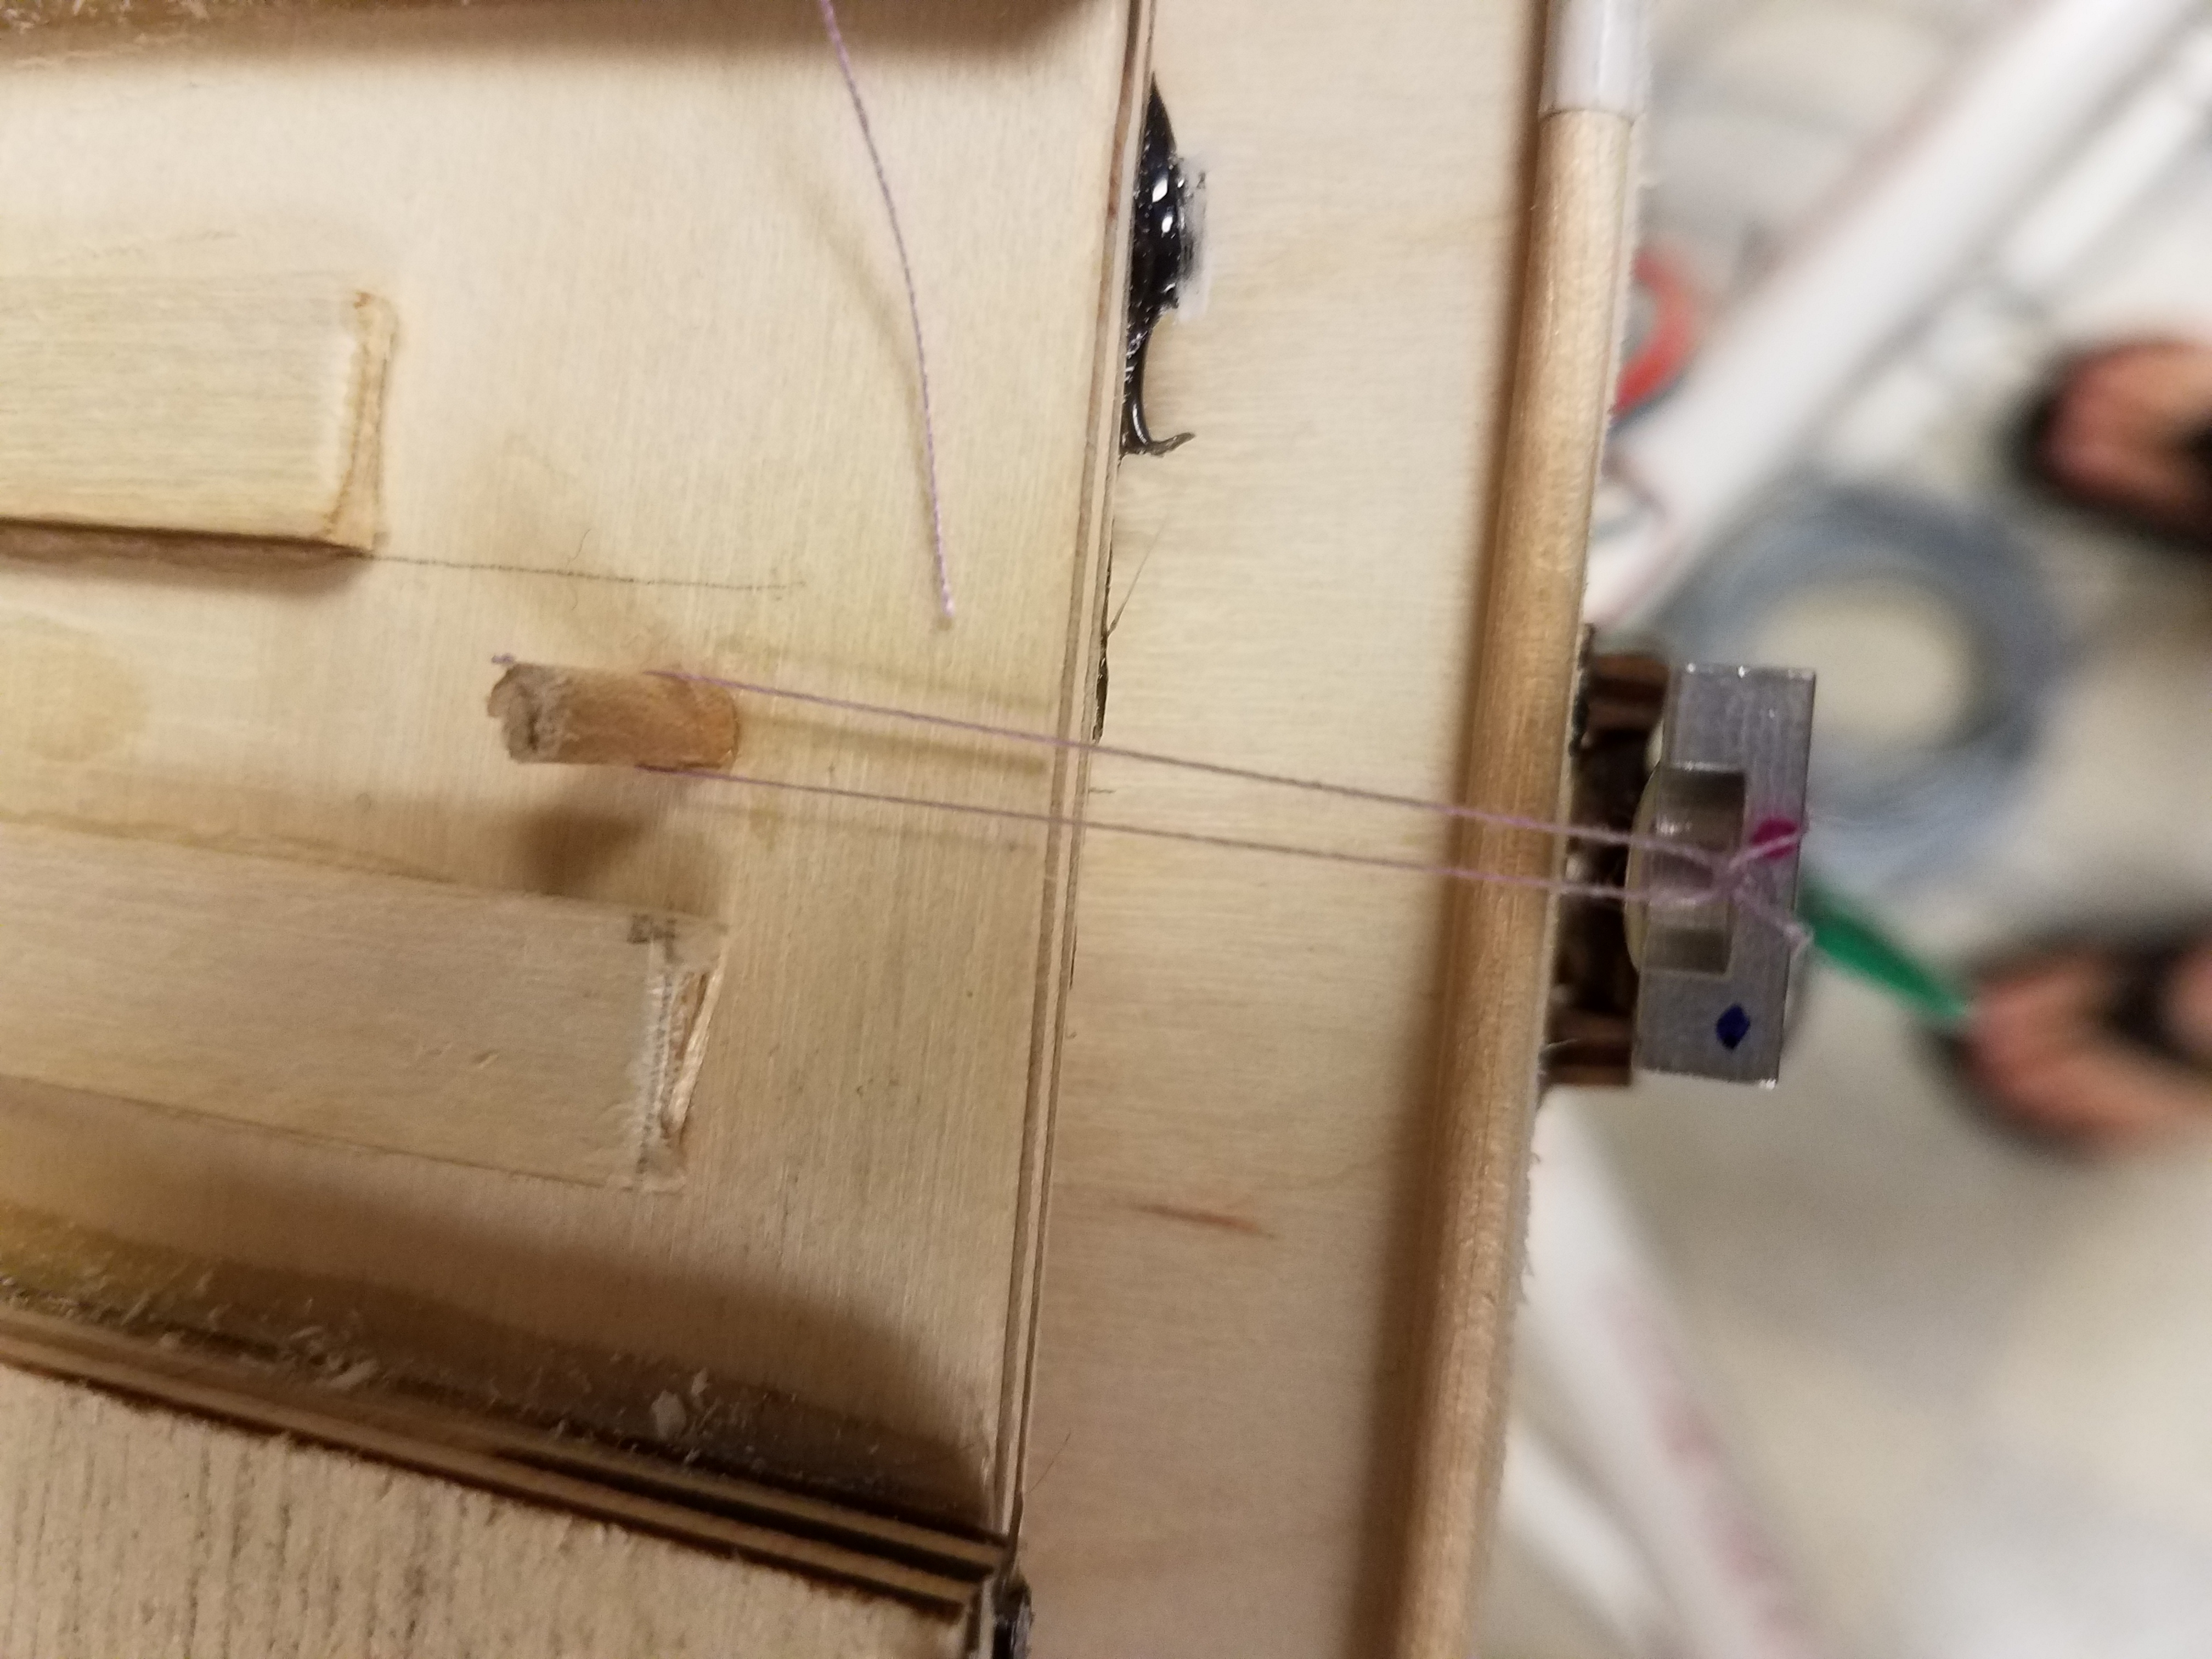
\includegraphics[angle = -90, width = 0.49\linewidth]{load_transfer.jpg}
\centering
\caption{Attachment of the load cell to the support structure for the first iteration drag experiment.}
\label{load_cell}
\end{figure}


However, after measuring the drag of the support structure, it turns out to be much higher than the expected drag of the sheet. Therefore,
it is necessary to reduce the drag in order to obtain accurate measurements of the sheet's drag. First, an effort was made to reduce the
drag of the existing structure by adding sharp trailing edges and rounded leading edges, instead of the original square corners. Paper was
creased to create a sharp edge, and taped to the trailing edge of the support frame (Figure \ref{sharp_edge}). Then, more paper was bent
into a semi-circle and taped to the leading edge. Thus, the cross section of each element of the frame is shaped roughly like an airfoil.
Furthermore, a smooth transition between segments with varying cross sections was produced. It is hoped that this will reduce the drag.

\begin{figure}
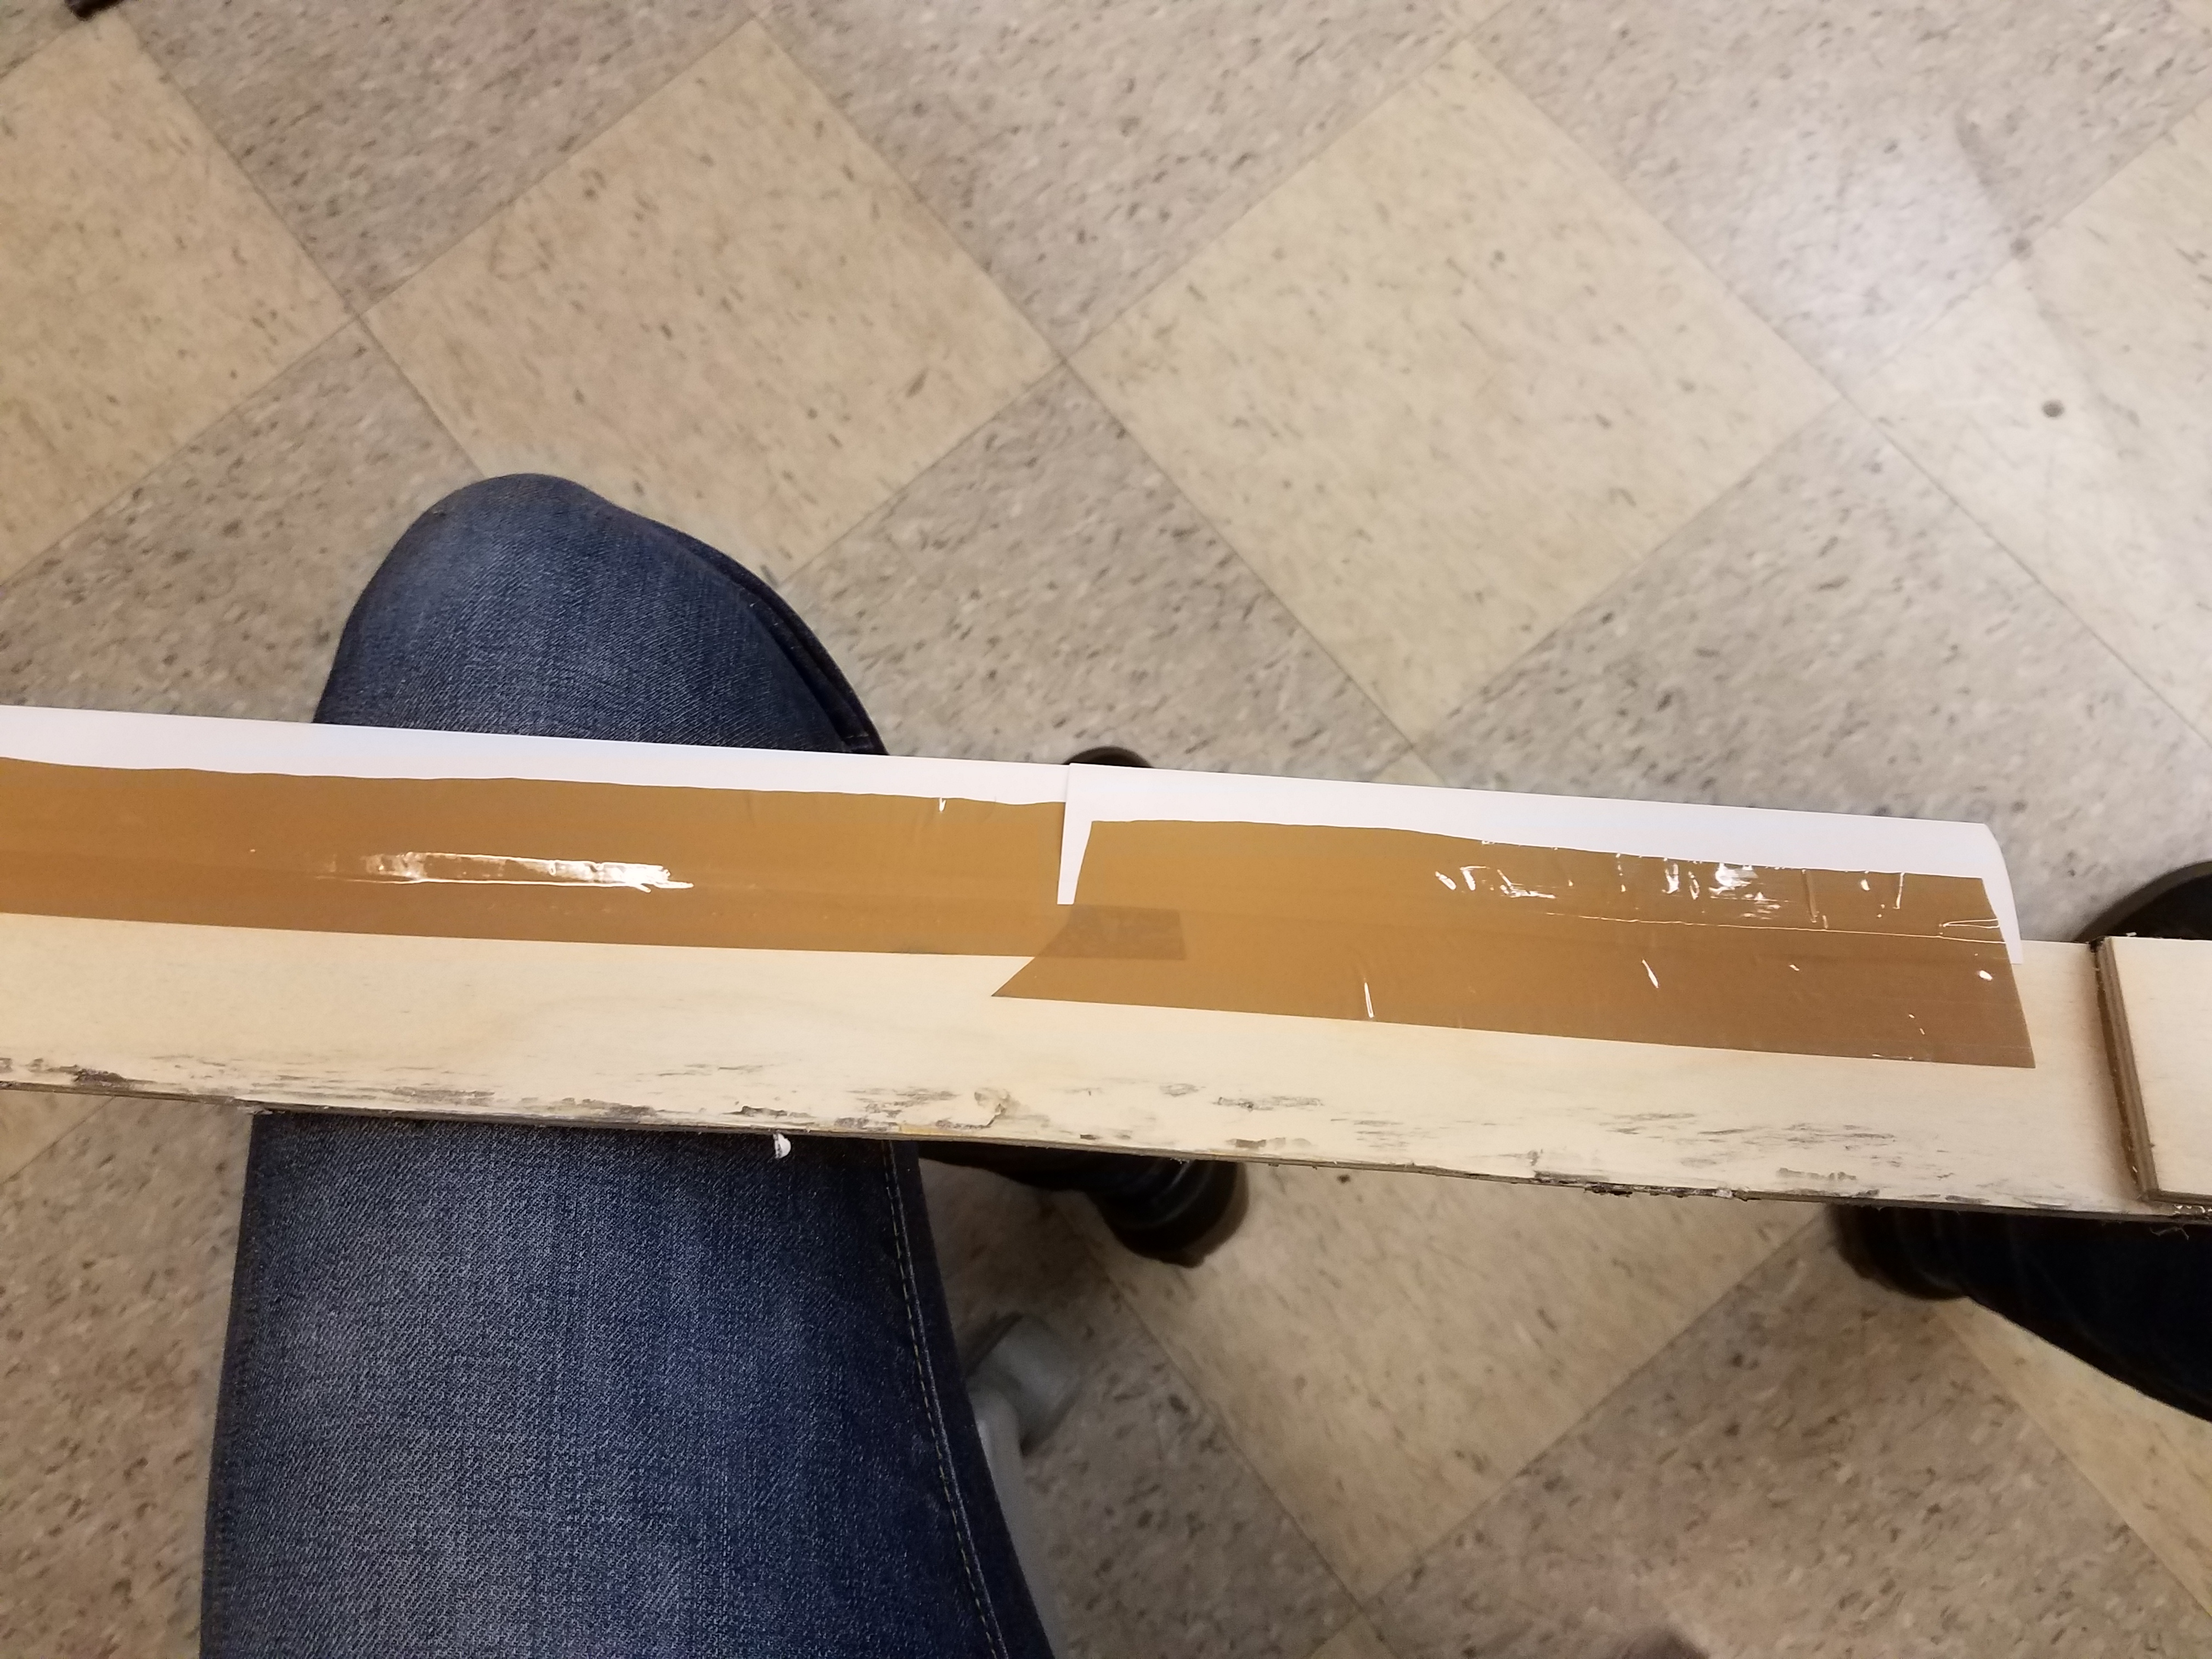
\includegraphics[width = 0.7\linewidth]{sharp_edge.jpg}
\centering
\caption{The attempt to reduce the drag of the frame by producing sharp trailing edges.}
\label{sharp_edge}
\end{figure}

Even still, while the frame was being retrofit with the leading and trailing edge devices, an alternative setup was proposed which is
expected to have essentially zero drag. The frame is enclosed in a housing which will essentially isolate it from the outside flow,
but still permit the strings which support the sheet to pass through. The frame will still be able to roll, so that the drag force
is transmitted from the sheet to the frame to the load cell. This concept and the progress on it so far is describe below in ``Second
Iteration''.

\subsubsection{First Iteration}
The sheet system is be suspended in the wind tunnel by a frame which holds the load cell and exhibits three flat surfaces, on which the
sheet's bearings roll. Figure \ref{frame_and_support} shows this setup.
The PVC pipes which comprise the structure of the frame are connected with friction-fitted pipe conections.
Consequently, the structure is completely modular, and any aspect of it can be modified simply by taking it apart, changing the pipe lengths,
and reassembling it. This may be useful if follow-up experiments require a slightly different setup. There is an extra joint in the rear pipe
so that a longer or shorter pipe can easily be substituted, and the spacing in the joint can be changed. This provides a means to
fine-tune the angle of attack. Figure \ref{support_structure} displays
the support structure by itself.

\begin{figure}
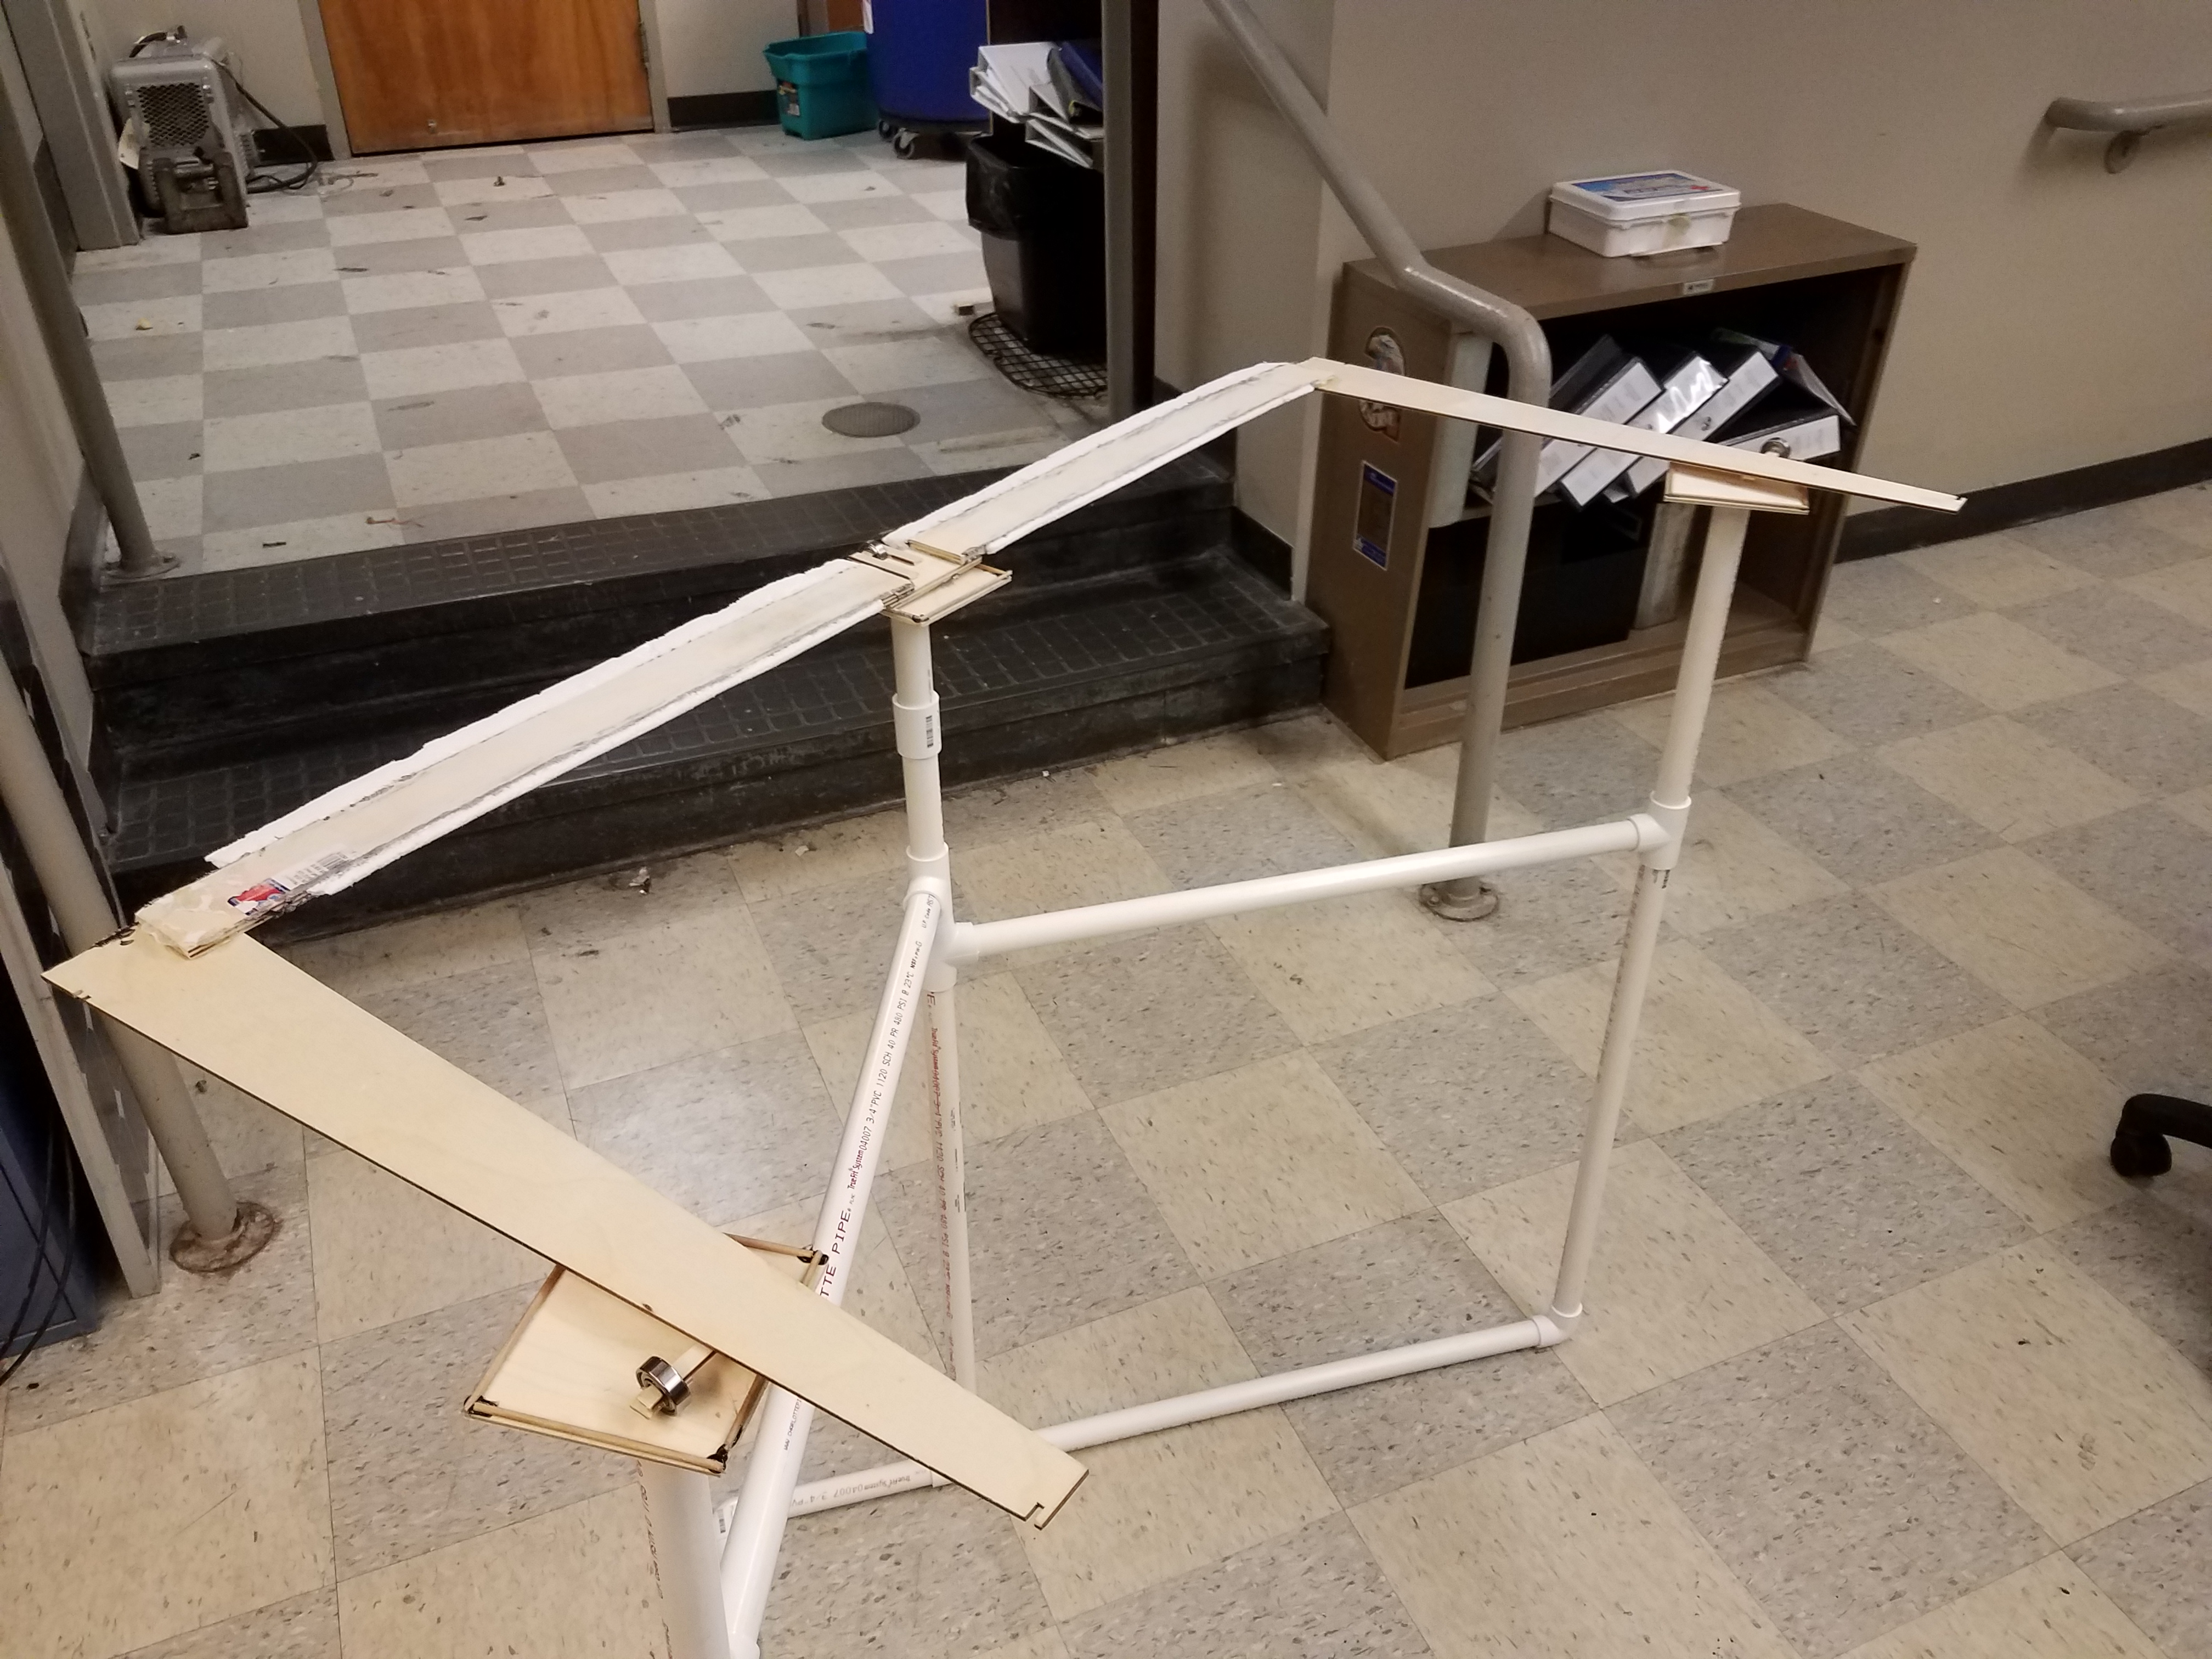
\includegraphics[width = 0.7\linewidth]{drag_setup.jpg}
\centering
\caption{The sheet frame and support structure assembly.}
\label{frame_and_support}
\end{figure}

\begin{figure}
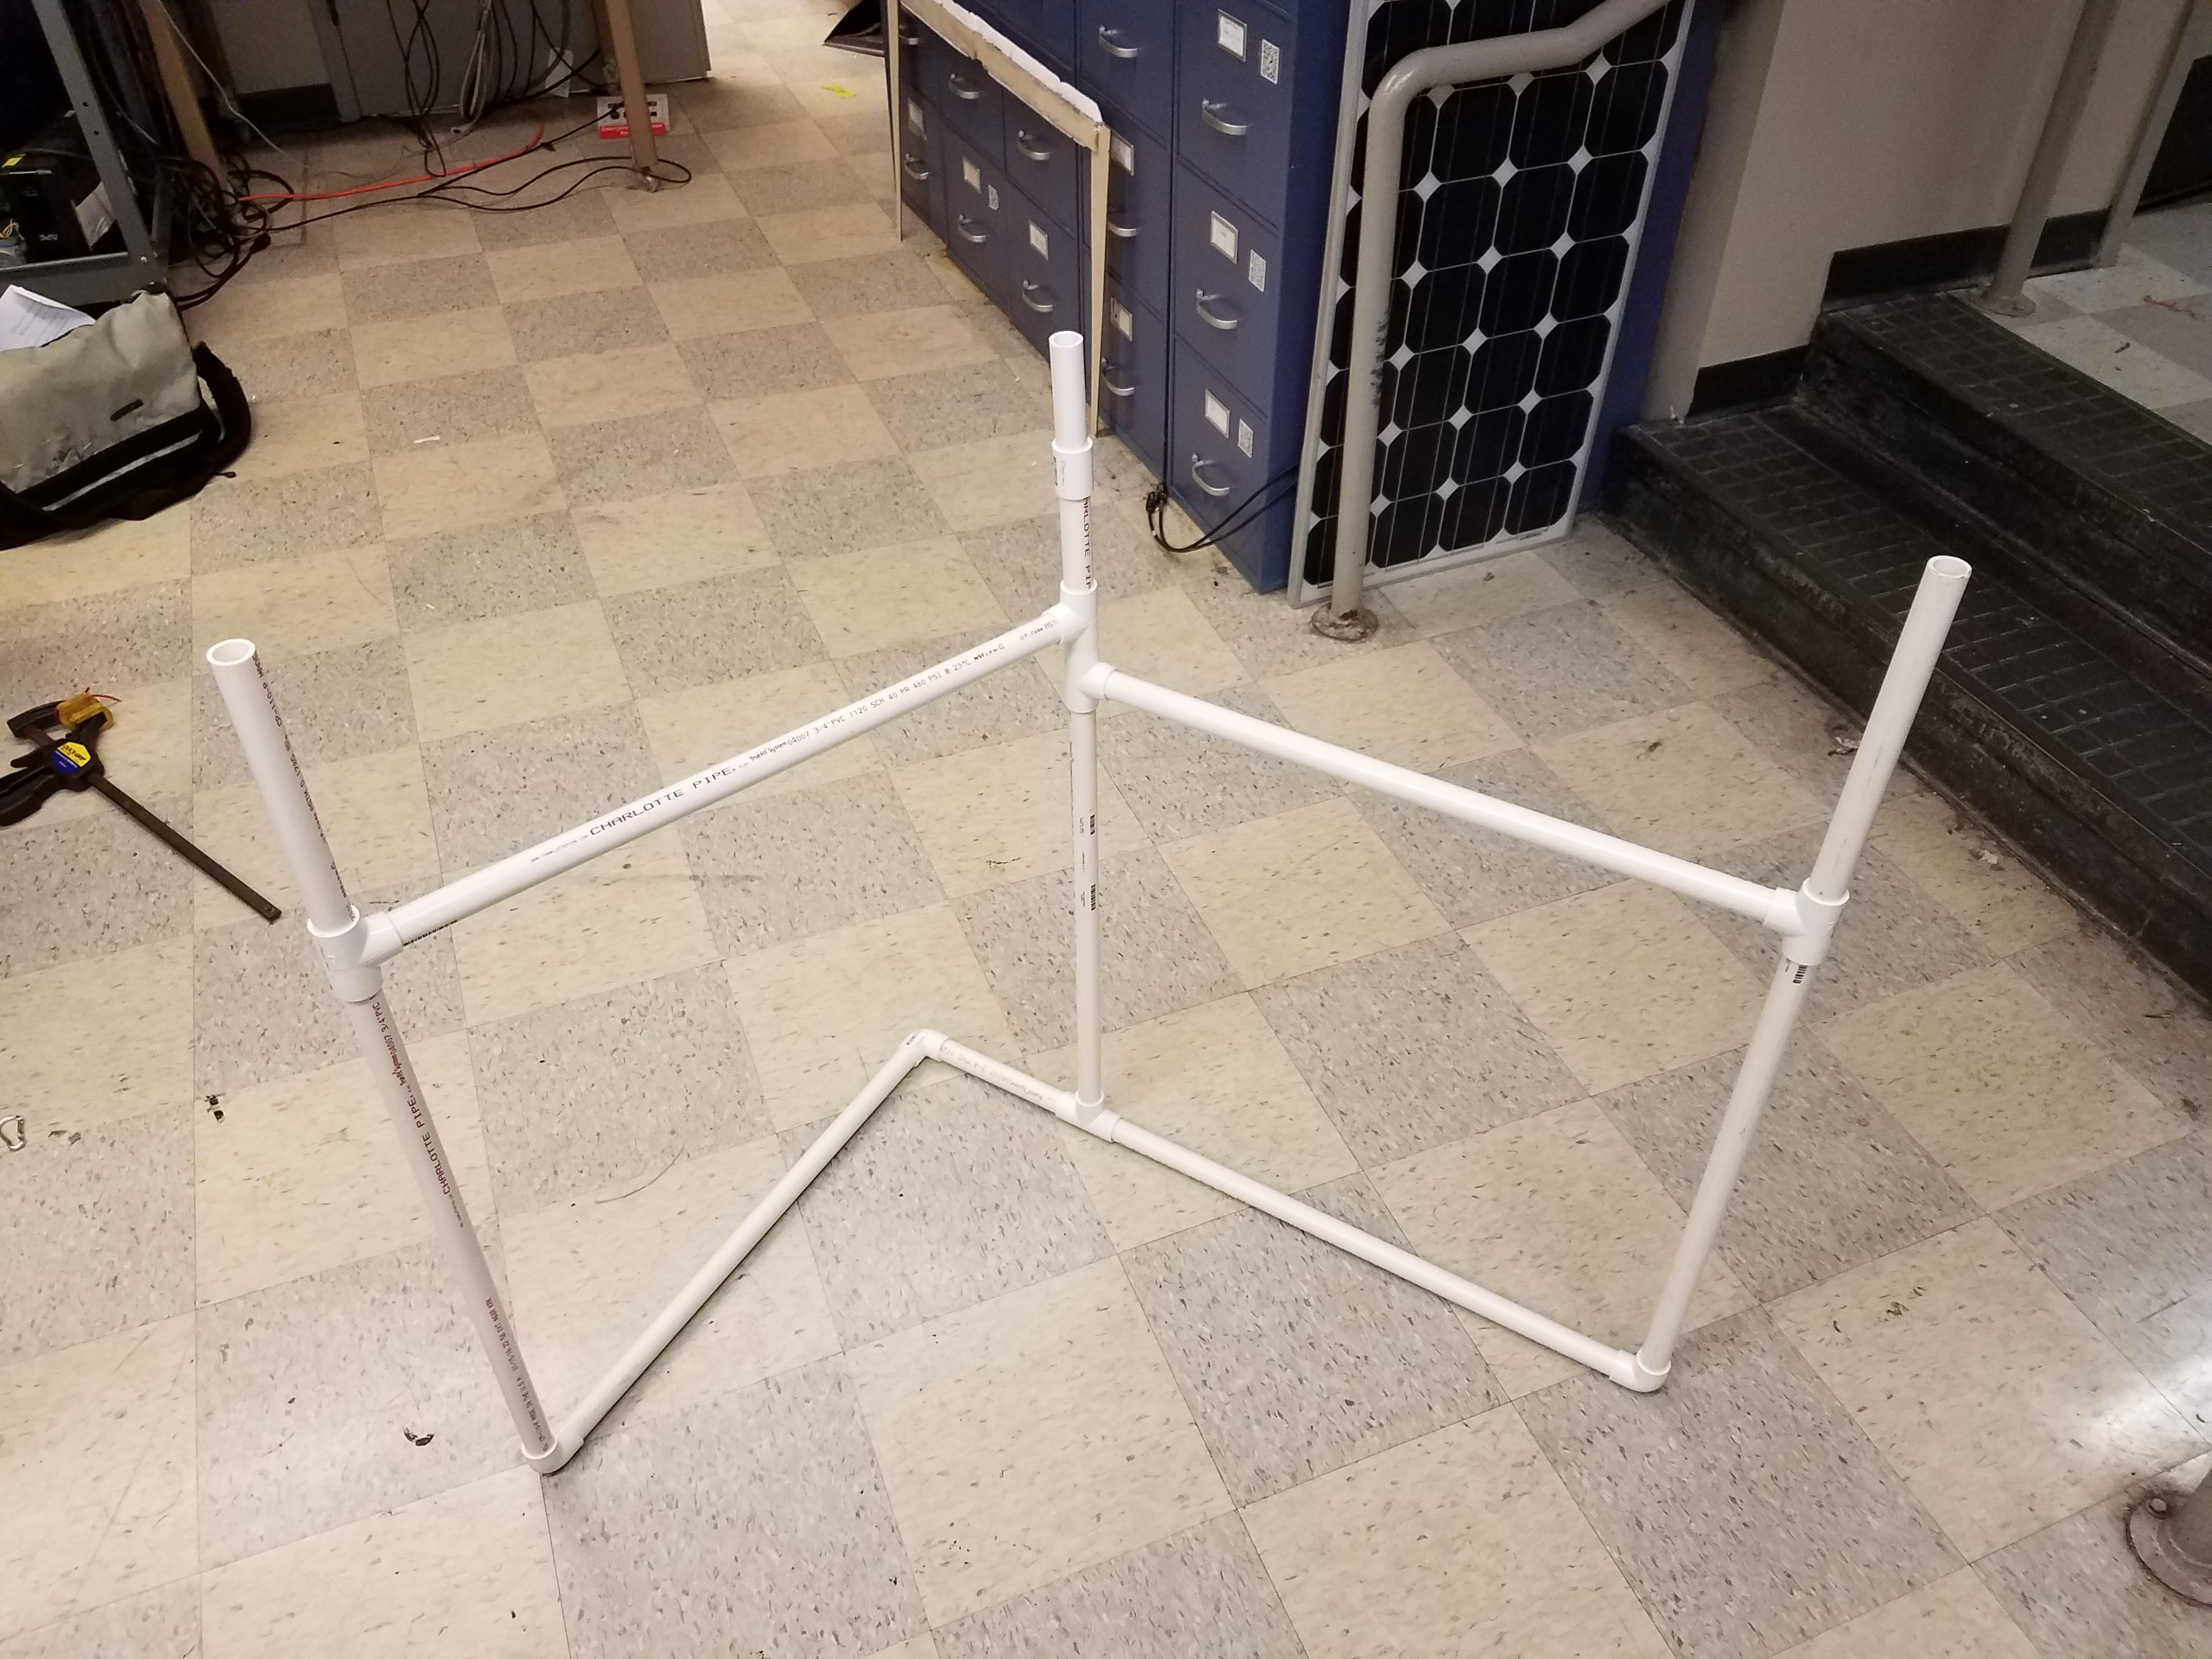
\includegraphics[width = 0.7\linewidth]{mount_structure.jpg}
\centering
\caption{The frame which will support the sheet system during drag measurements}
\label{support_structure}
\end{figure}

The interface between the support structure and the sheet received most of the attention during the manufacturing process.
The sheet's roller bearings must roll on three flat surfaces on the support structure. One of these interfaces is shown in
figure \ref{roller}. The rolling surface mainly consists of a $4 in \times 4 in$ square of $1/8 in$ thick plywood. Four $1/8
in$ diameter wooden dowels were fixed to the edges using hot glue in order to prevent the roller from accidently rolling off
the surface. The subassembly of the plywood and dowels, shown in Figure \ref{surface}, was attached to the end of its
respective PVC pipe in the structure by means of hot glue.

\begin{figure}
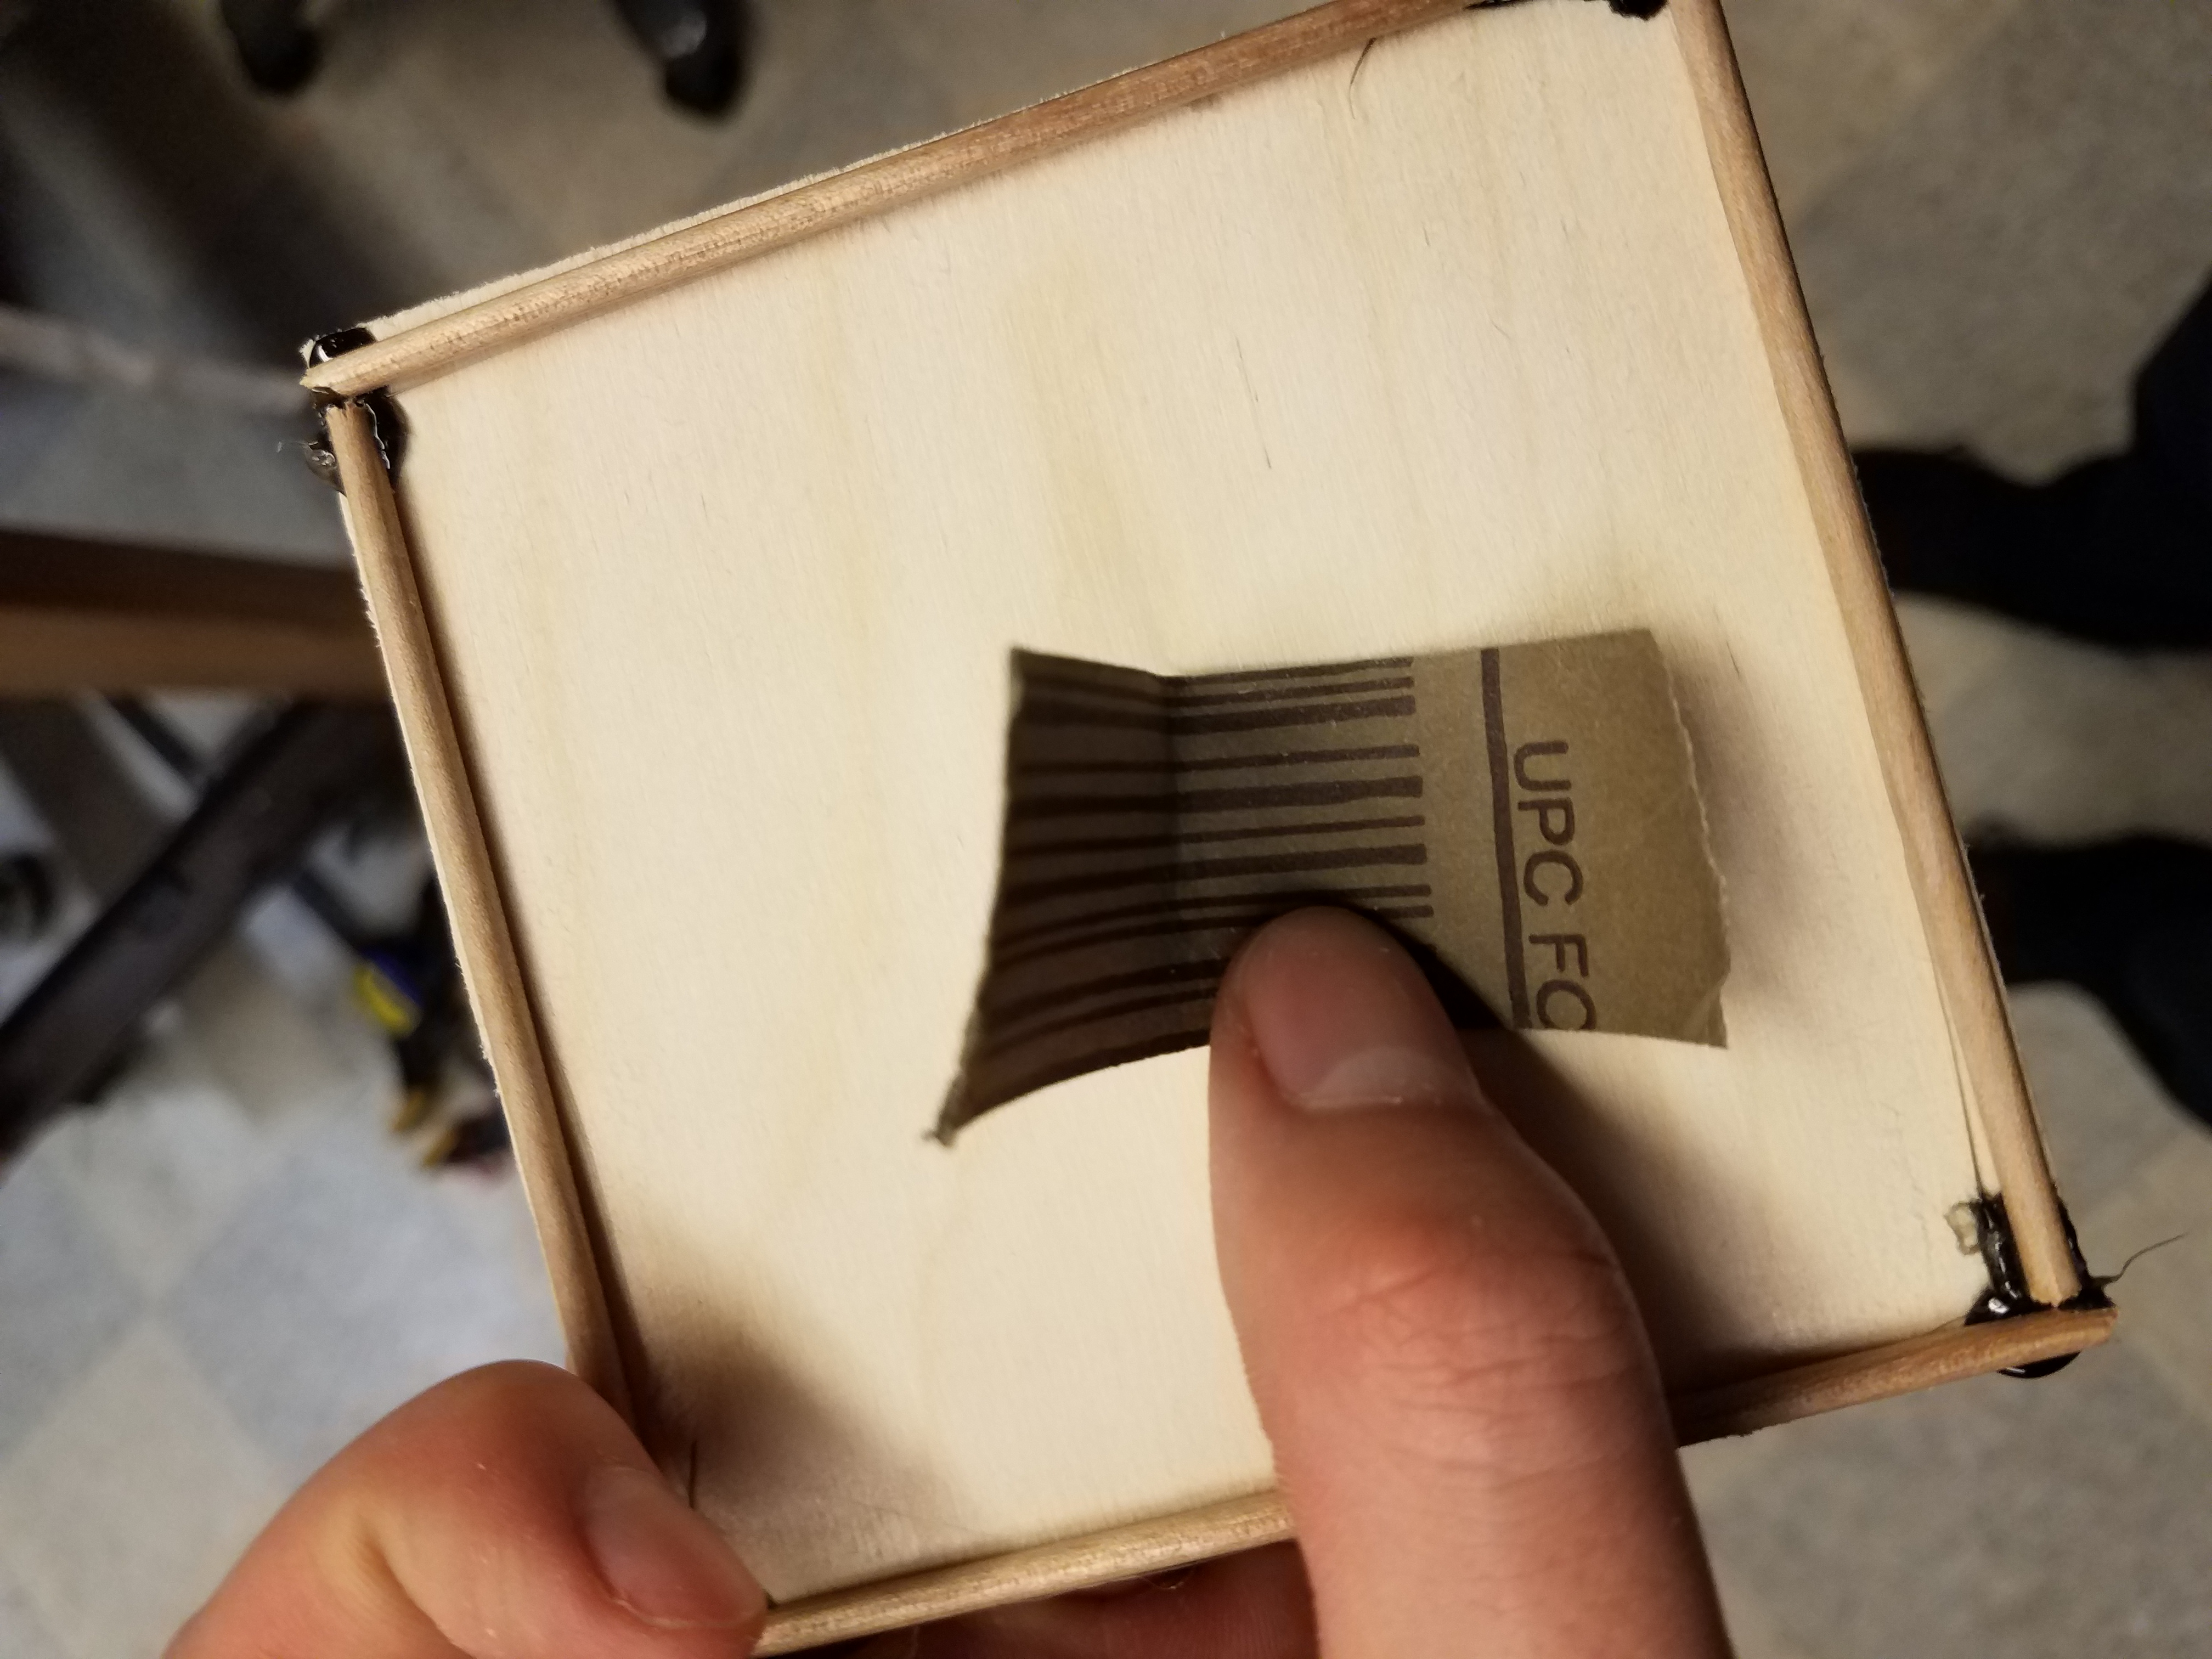
\includegraphics[width = 0.7\linewidth]{sanding.jpg}
\centering
\caption{The surface which the sheet frame rolls on while being sanded to decrease roughness.}
\label{surface}
\end{figure}

\begin{figure}
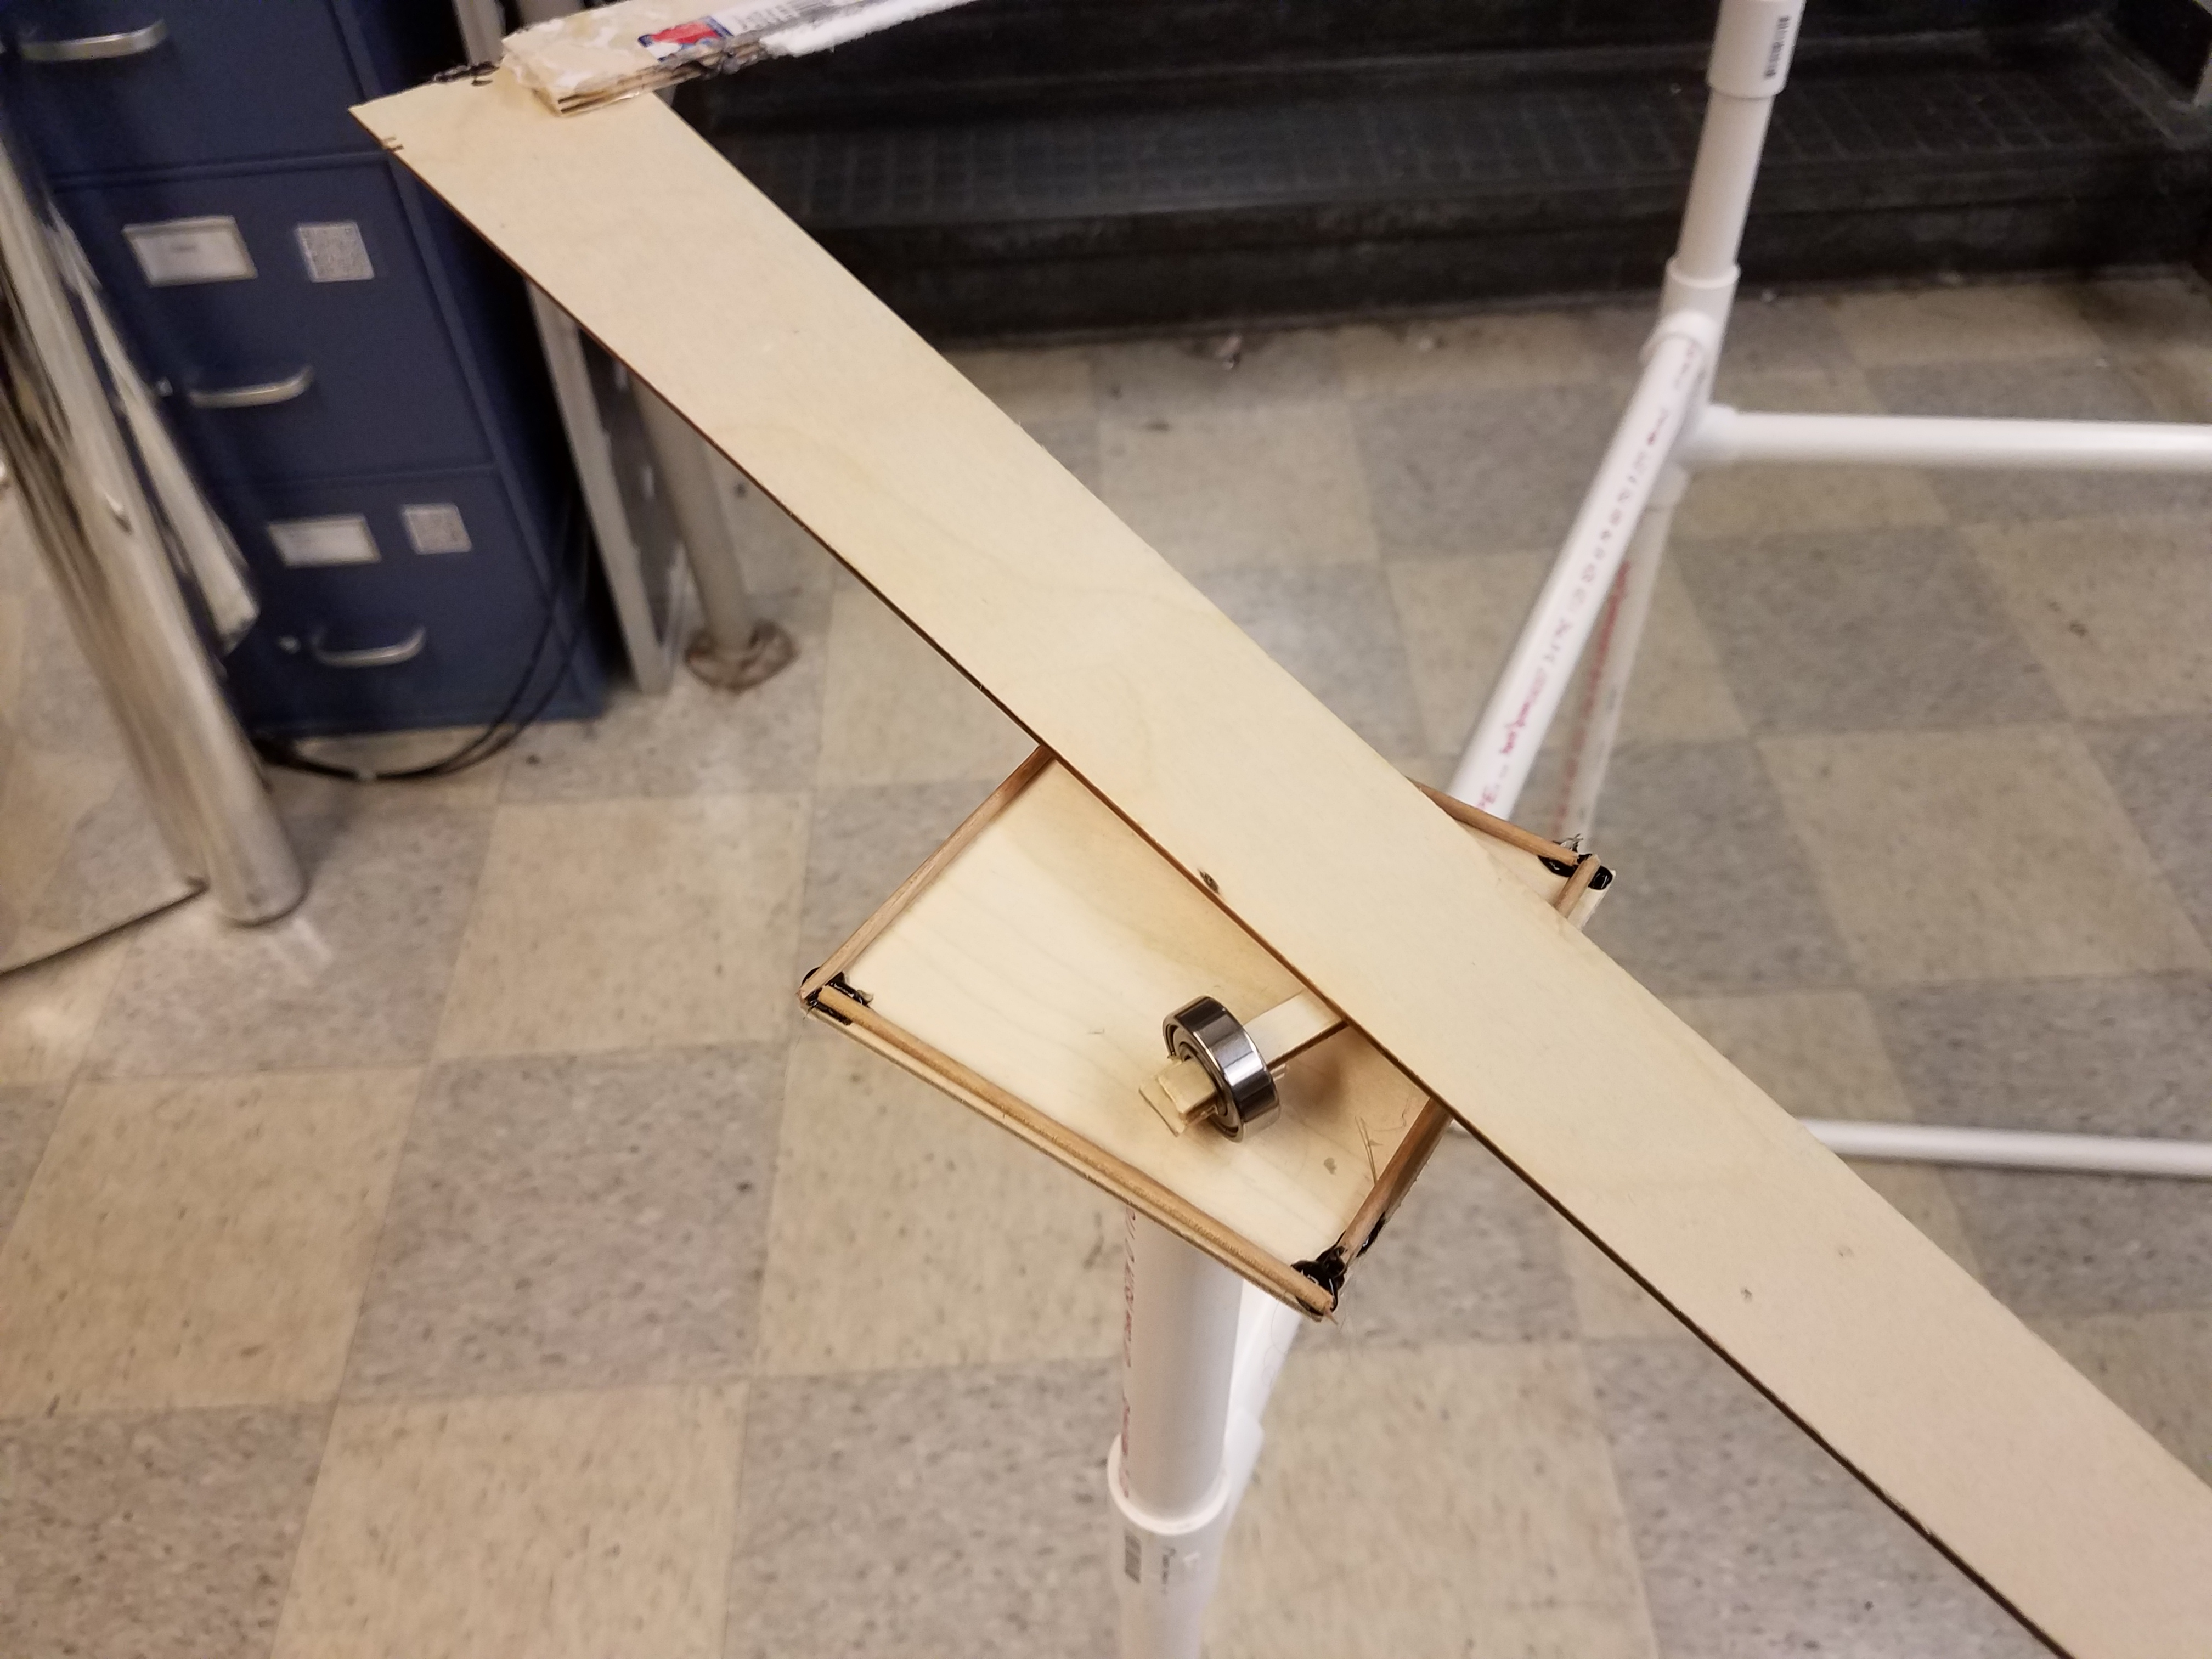
\includegraphics[width = 0.7\linewidth]{roller.jpg}
\centering
\caption{How the sheet frame rolls on the support structure.}
\label{roller}
\end{figure}

If these surfaces are not exactly level, then our drag measurements will be offset by $(w)sin(\theta)$,
where $w$ is the weight of the sheet and frame (minus the lift, if there is any) and $\theta$ is a weighted average of the
tilt angle of each of the surfaces. We attempt to correct for this offset by applying known loads to the sheet frame and measuring
the force on the load cell, because the force measured must always be the force applied plus a constant, which we may take to be
$(w)sin(\theta)$. However, before a systematic error is corrected for, it is better to attempt to reduce it first. Therefore,
it was attempted to make each rolling surface as level as possible. Each of the pipes which terminates in a rolling surface was
treated to ensure that the face at its end is even and normal to its axis. To that end, a sheet of paper was wrapped around
the pipe so that its edge is a straight line on the surface of the pipe whose ends joint. Thus the plane containing the line must
be normal to the axis of the pipe. The edge of the paper was marked on the pipe, and the end of the pipe was filed down to coincide
with the mark. This process is illustrated in Figure \ref{end_normalizing}. However, even still, the surfaces were not completely
level. This may be attributed to the flexibility and inadequate straightness of the PVC pipes. This could have been solved by using
a more rigid material, but that would have been more expensive and taken longer to construct. Furthermore, the amound of
tilt error appears to be less than the friction error (see below), because when placed on the rolling surfaces, the sheet frame
usually does not roll on its own. Therefore, the tilt error will be ignored for now.

\begin{figure}
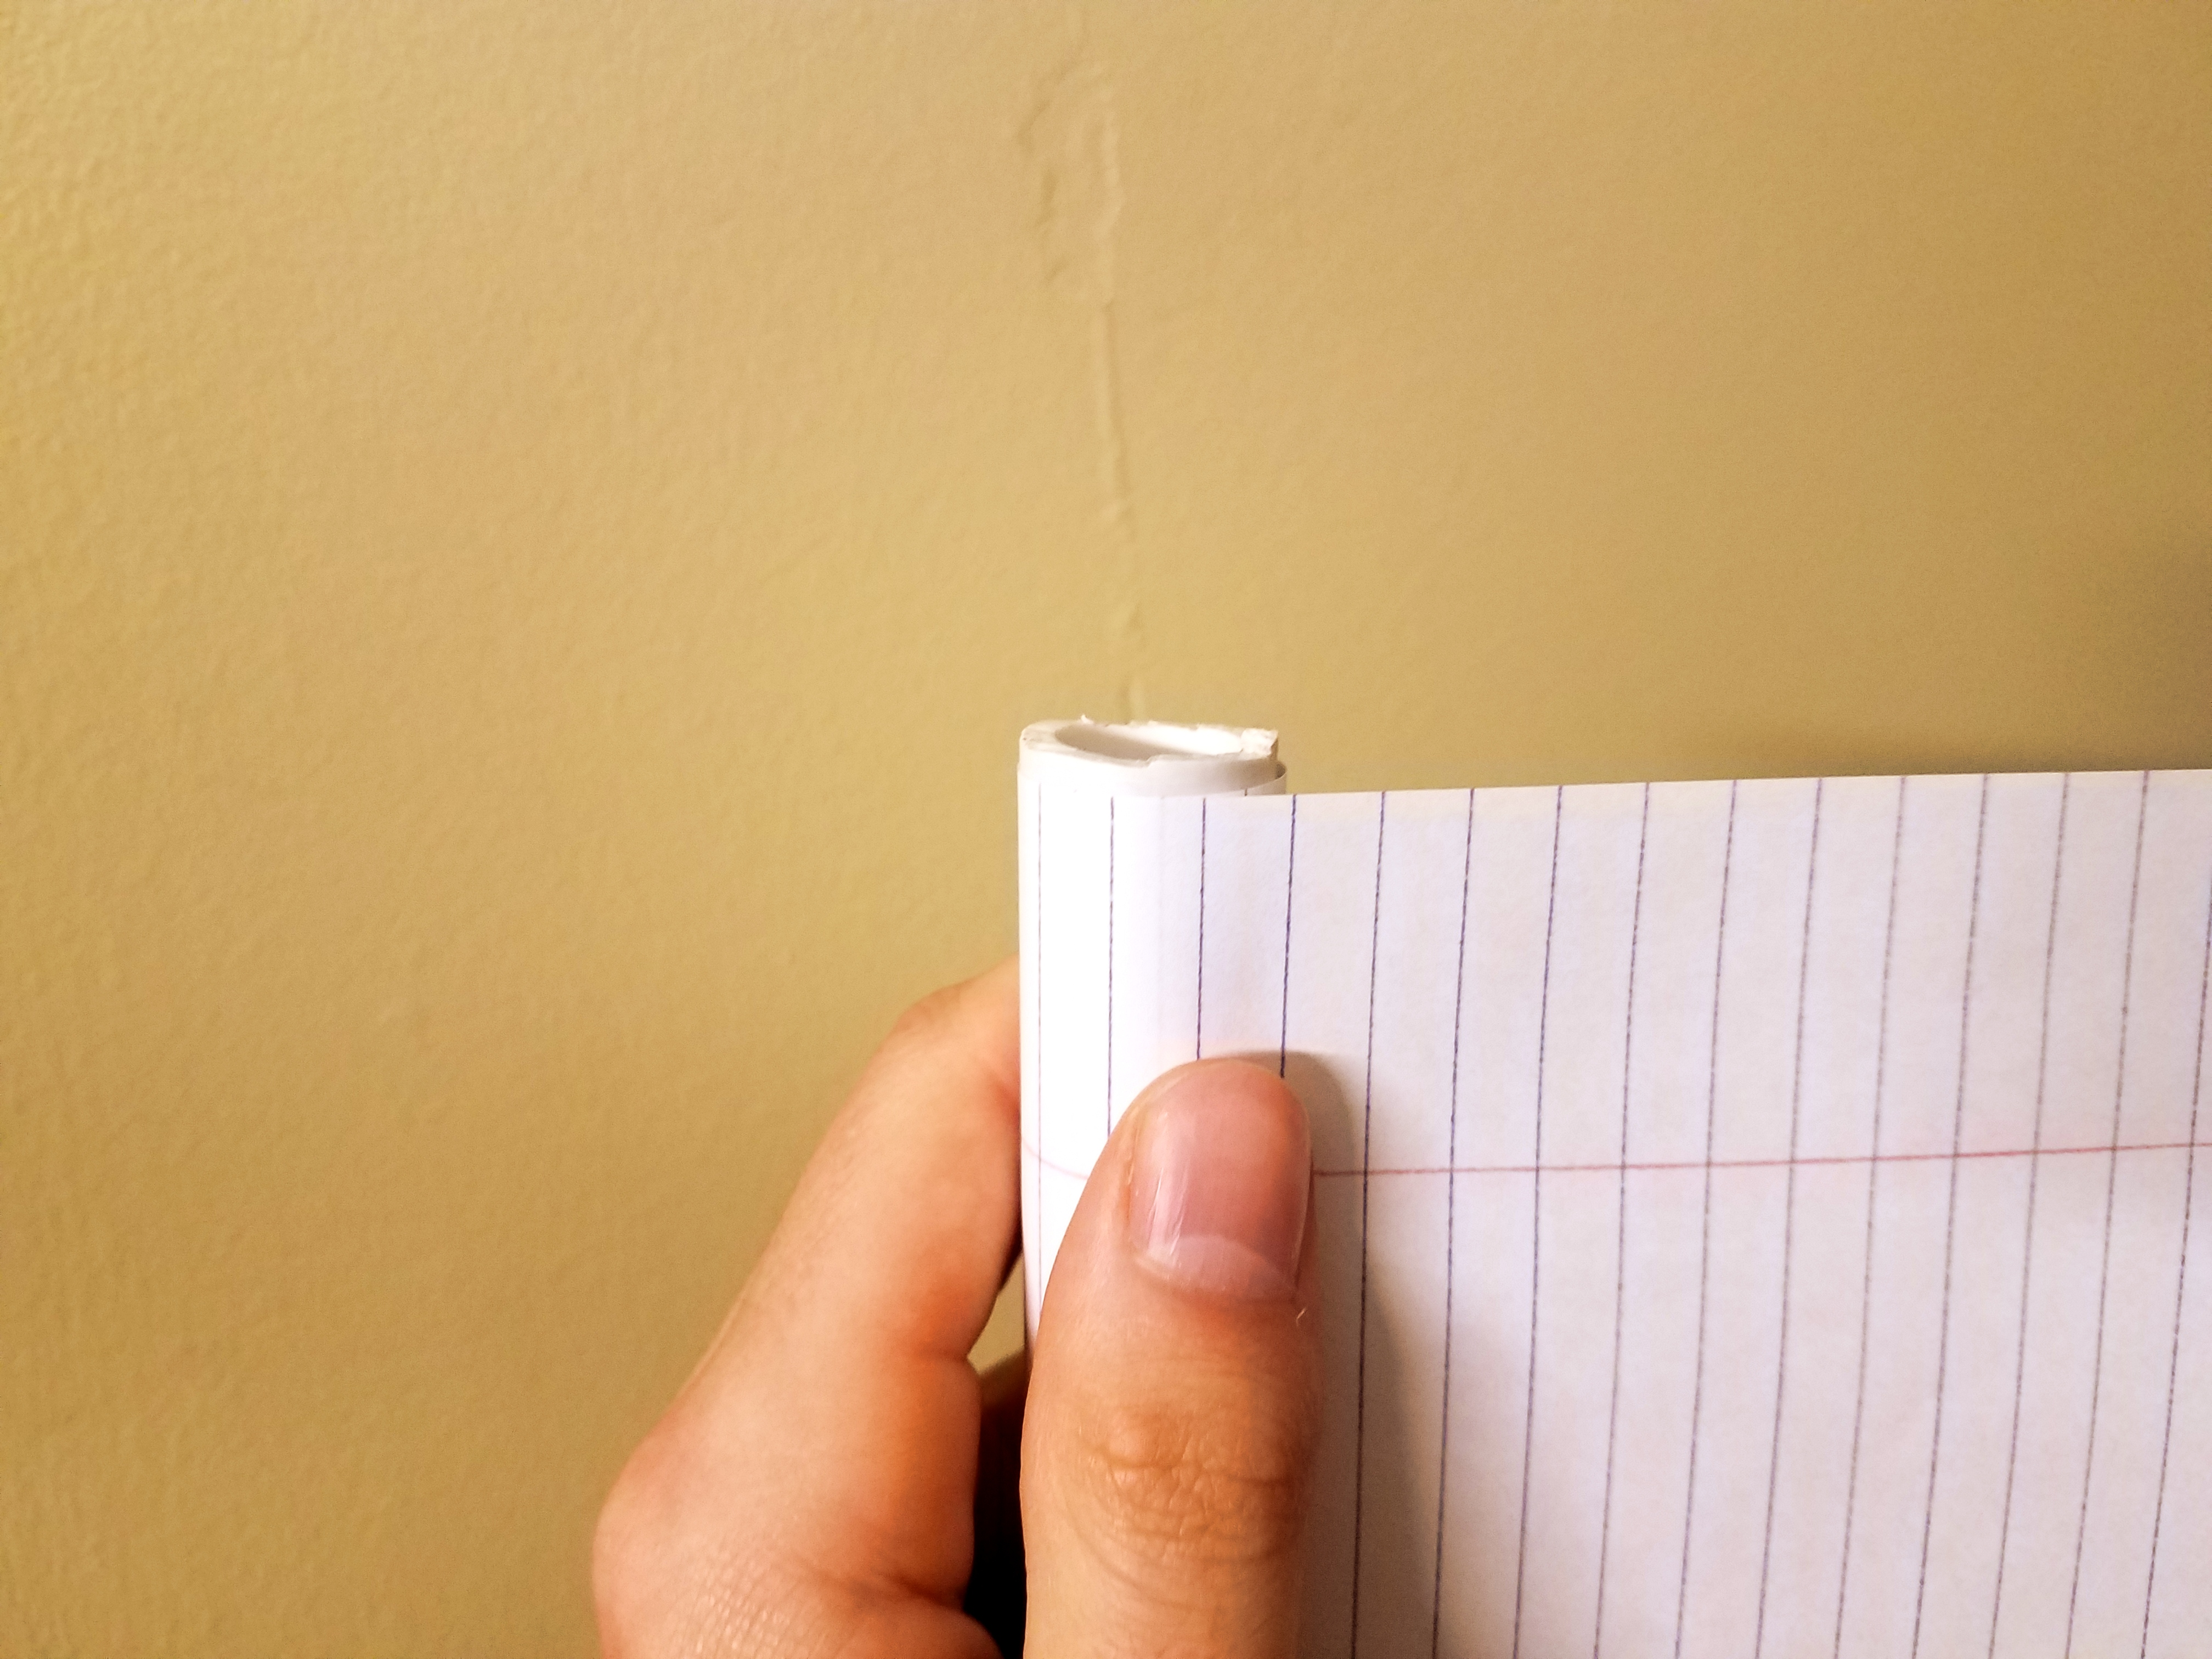
\includegraphics[width = 0.49\linewidth]{perpendicular.jpg}
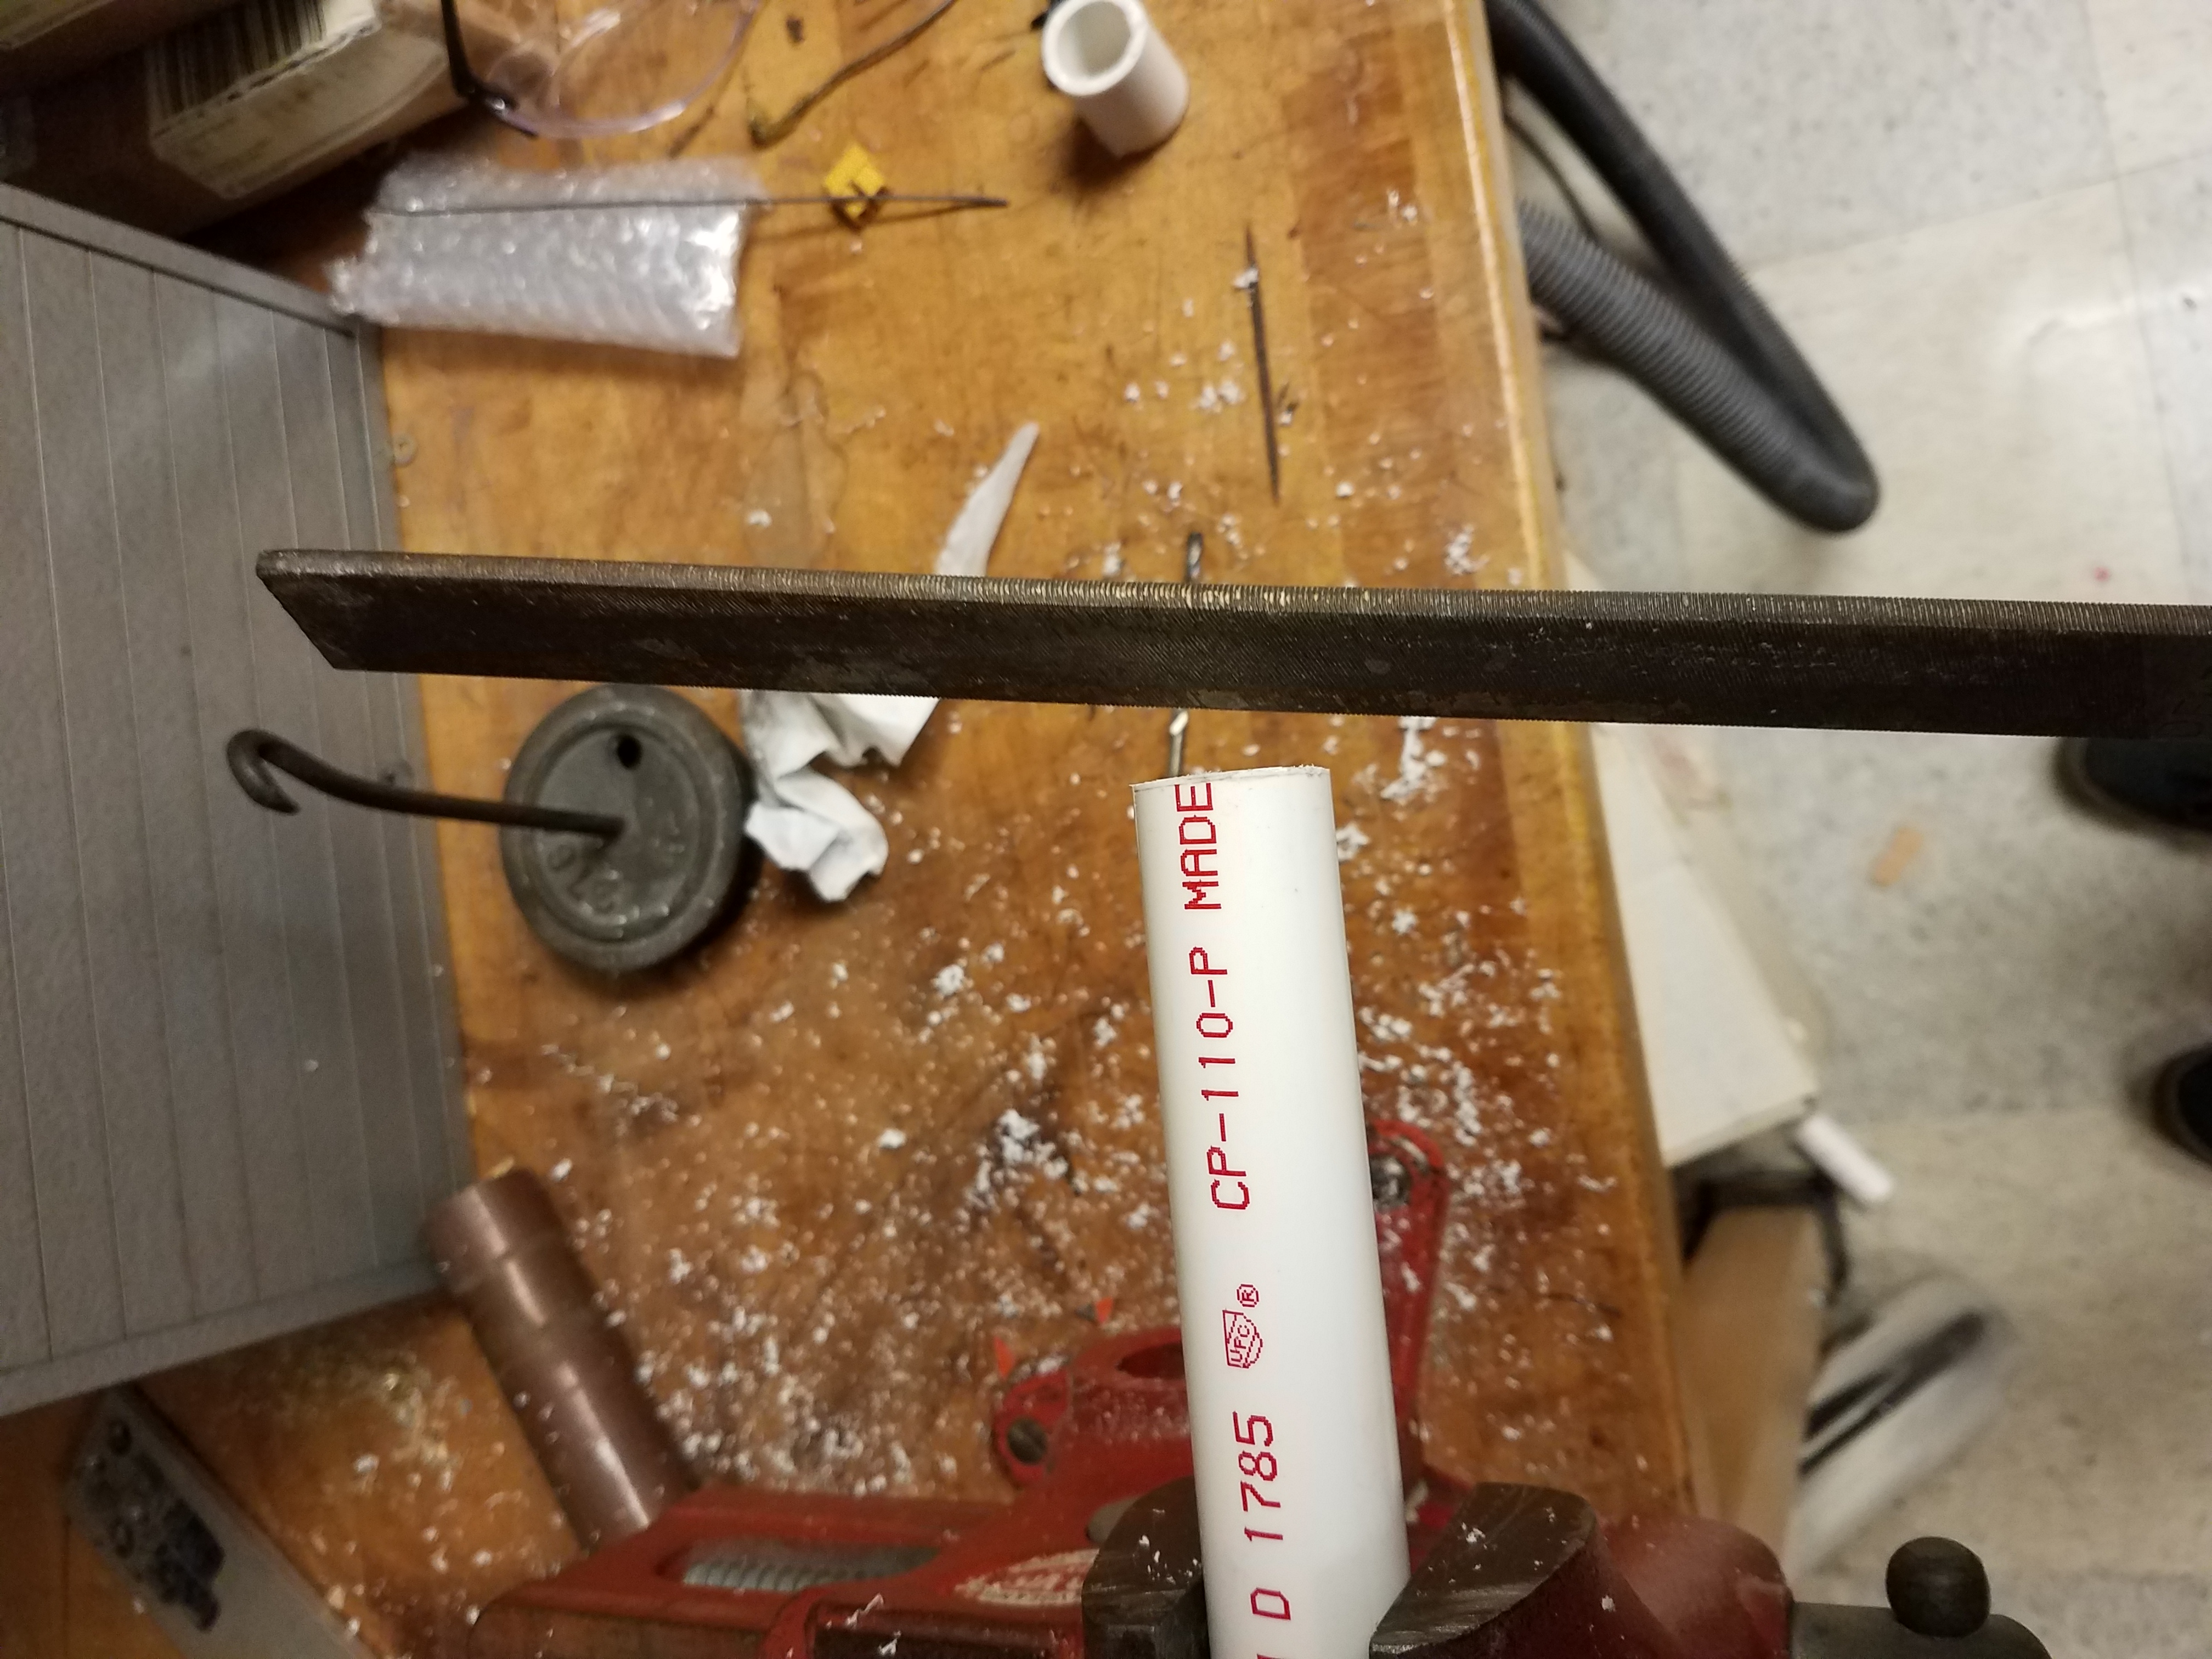
\includegraphics[width = 0.49\linewidth]{leveling.jpg}
\centering
\caption{Ensuring that each pipe end which will be glued to a surface is level.}
\label{end_normalizing}
\end{figure}

Even more important than the tilt error is the friction error, which cannot be easily corrected for. There are two ways in which
friction in the assembly results in error in the force measurements. First, the roller bearings have internal friction. However,
the manufacturer has designed them to minimize this, and little can be done to reduce it at this stage. Second, if the axes of the
three roller bearings are not exactly parallel, then there will be some friction between each bearing and the rolling surface,
since they cannot all simultaneously engage in pure rolling. The component of the friction force which causes error in the
measurements will be proportional to the sine of the error in the angle alignment. However, there is one additional cause of
force error which will also be referred to as ``friction error'', namely, roughness of the rolling surface. If there is a small
raised region on the rolling surface (i.e. a ``bump''), then it will require additional force to pull the roller over it. This
additional force will have the same effect as increasing the static friction coefficient, so all three of the phenomena
above will fall under the category of friction error in this report.

In order to reduce friction error, there must be a means to assess it. As an interim measure, before the load cell measurement
technique was fully developed, a mechanical method based on Hooke's Law was devised to measure friction (Figure \ref{friction}).
A thin rubber band was fixed to a plate at one end and tied to a thread on the other end, such that the band is parallel to the
plate. A mark was made near the free
end of the relaxed rubber band and at the coinciding point on the plate. A 7.5 oz weight was hung from
the thread, and the displacement of the free end of the rubber band was measured. Assuming linear elasticity, the displacement
of the rubber band under the minimum expected drag force, 0.14 N (see ``Force Predictions'' above), was calculated, and a mark
corresponding to that displacement was made on the plate. Therefore, if a force is applied to the rubber band, as long as the
mark on the rubber band does not reach the second mark on the plate, the applied force must be less than the minimum expected
drag force, which the experiment is designed to measure.

As soon as the frame and support structure was complete, the sheet was attached to the rubber band measurement device, and the
rubber band was slowly stretched until the sheet frame began to accelerate. Depending on the position of the rollers
on the rolling surface, the rubber band was stretched somewhere between $20\%$ and $100\%$ of the distance to the 0.14 N mark,
indicating far too much friction. Since the internal friction of the bearings and the friction due to misalignment were difficult
to reduce at this stage, an attempt was made to reduce the unevenness of the rolling surface. First, it was observed that the
hot glue gun had left filaments of adhesive material on the rolling surface, and these filaments were removed. Second, the surface
was sanded to remove roughness caused by the grain of the wood. After sanding, the rubber band test was applied again. This time,
the force required to start the sheet frame rolling was so small that it was impossible to assess acurately with this low-
fidelity technique. The unsteadyness of the hand holding the instrumet combined with the inertia of the sheet caused the
displacement to fluctuate, so
that it was hard to pinpoint the exact value. However, my best judgement is that the friction error is probably less than $10\%$
(perhaps much less, but it is impossible to say). In any case, the roller system can certainly detect the minimum drag we
need to measure, although in order to determine the accuracy of the measurements we will need to use the load cell.


\begin{figure}
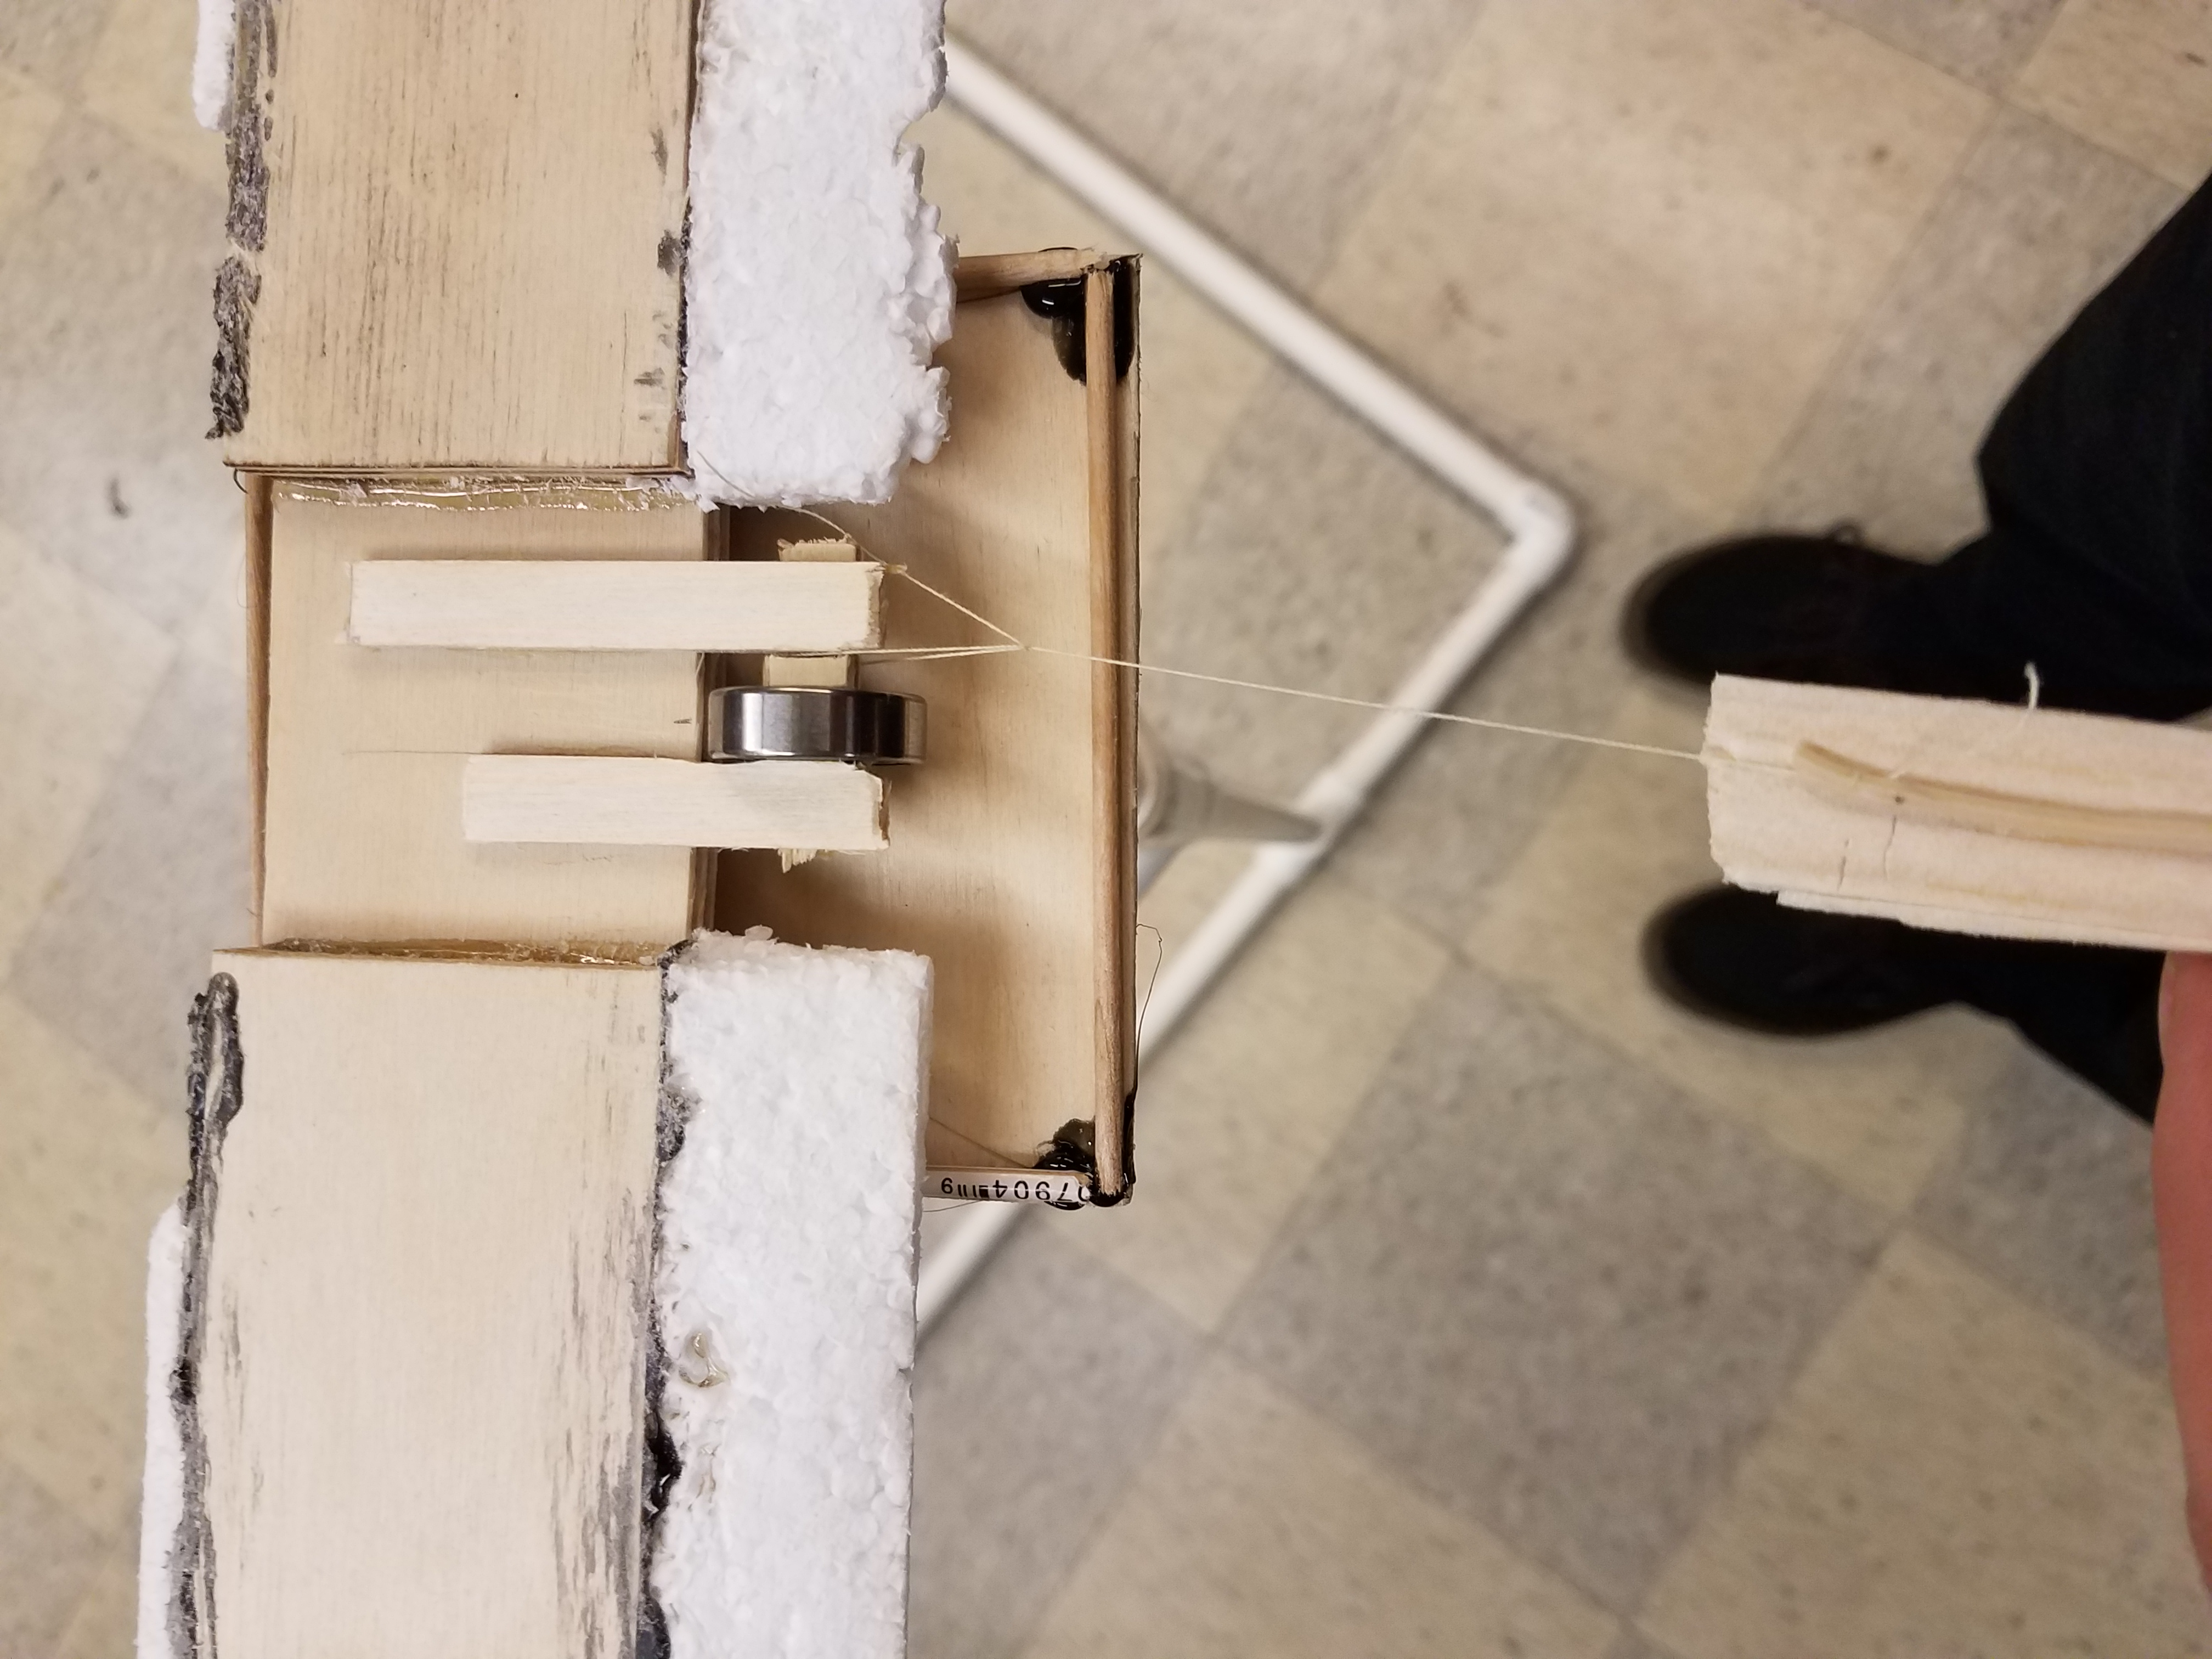
\includegraphics[width = 0.7\linewidth]{sensitivity.jpg}
\centering
\caption{Measuring the friction in the roller system. The sheet was at the verge of rolling when this photograph was taken.}
\label{friction}
\end{figure}

In addition to the tilt and friction error, another source of eror has become apparent, but unlike the other two it is not
a flaw in the force measurement system, but an error in the drag force itself. The entire sheet frame is twisted, as can be
seen in Figure \ref{skewness}. This appears to be a result of warping of the plywood from which the frame is constructed.
This problem could have been avoided by making the main structure of the frame have the cross section of a box, rather than
a single sheet, but a box would have dramatically more drag. Instead, the twist can be corrected by placing 2 oz of dead weight
on the left (port) side of the frame (Figure \ref{skewness_correction}). Since an extra object there will cause extra drag,
interfering with the measurements,
some kind of faring must be constructed to reduce the extra drag. That is intended to happen this coming week.

\begin{figure}
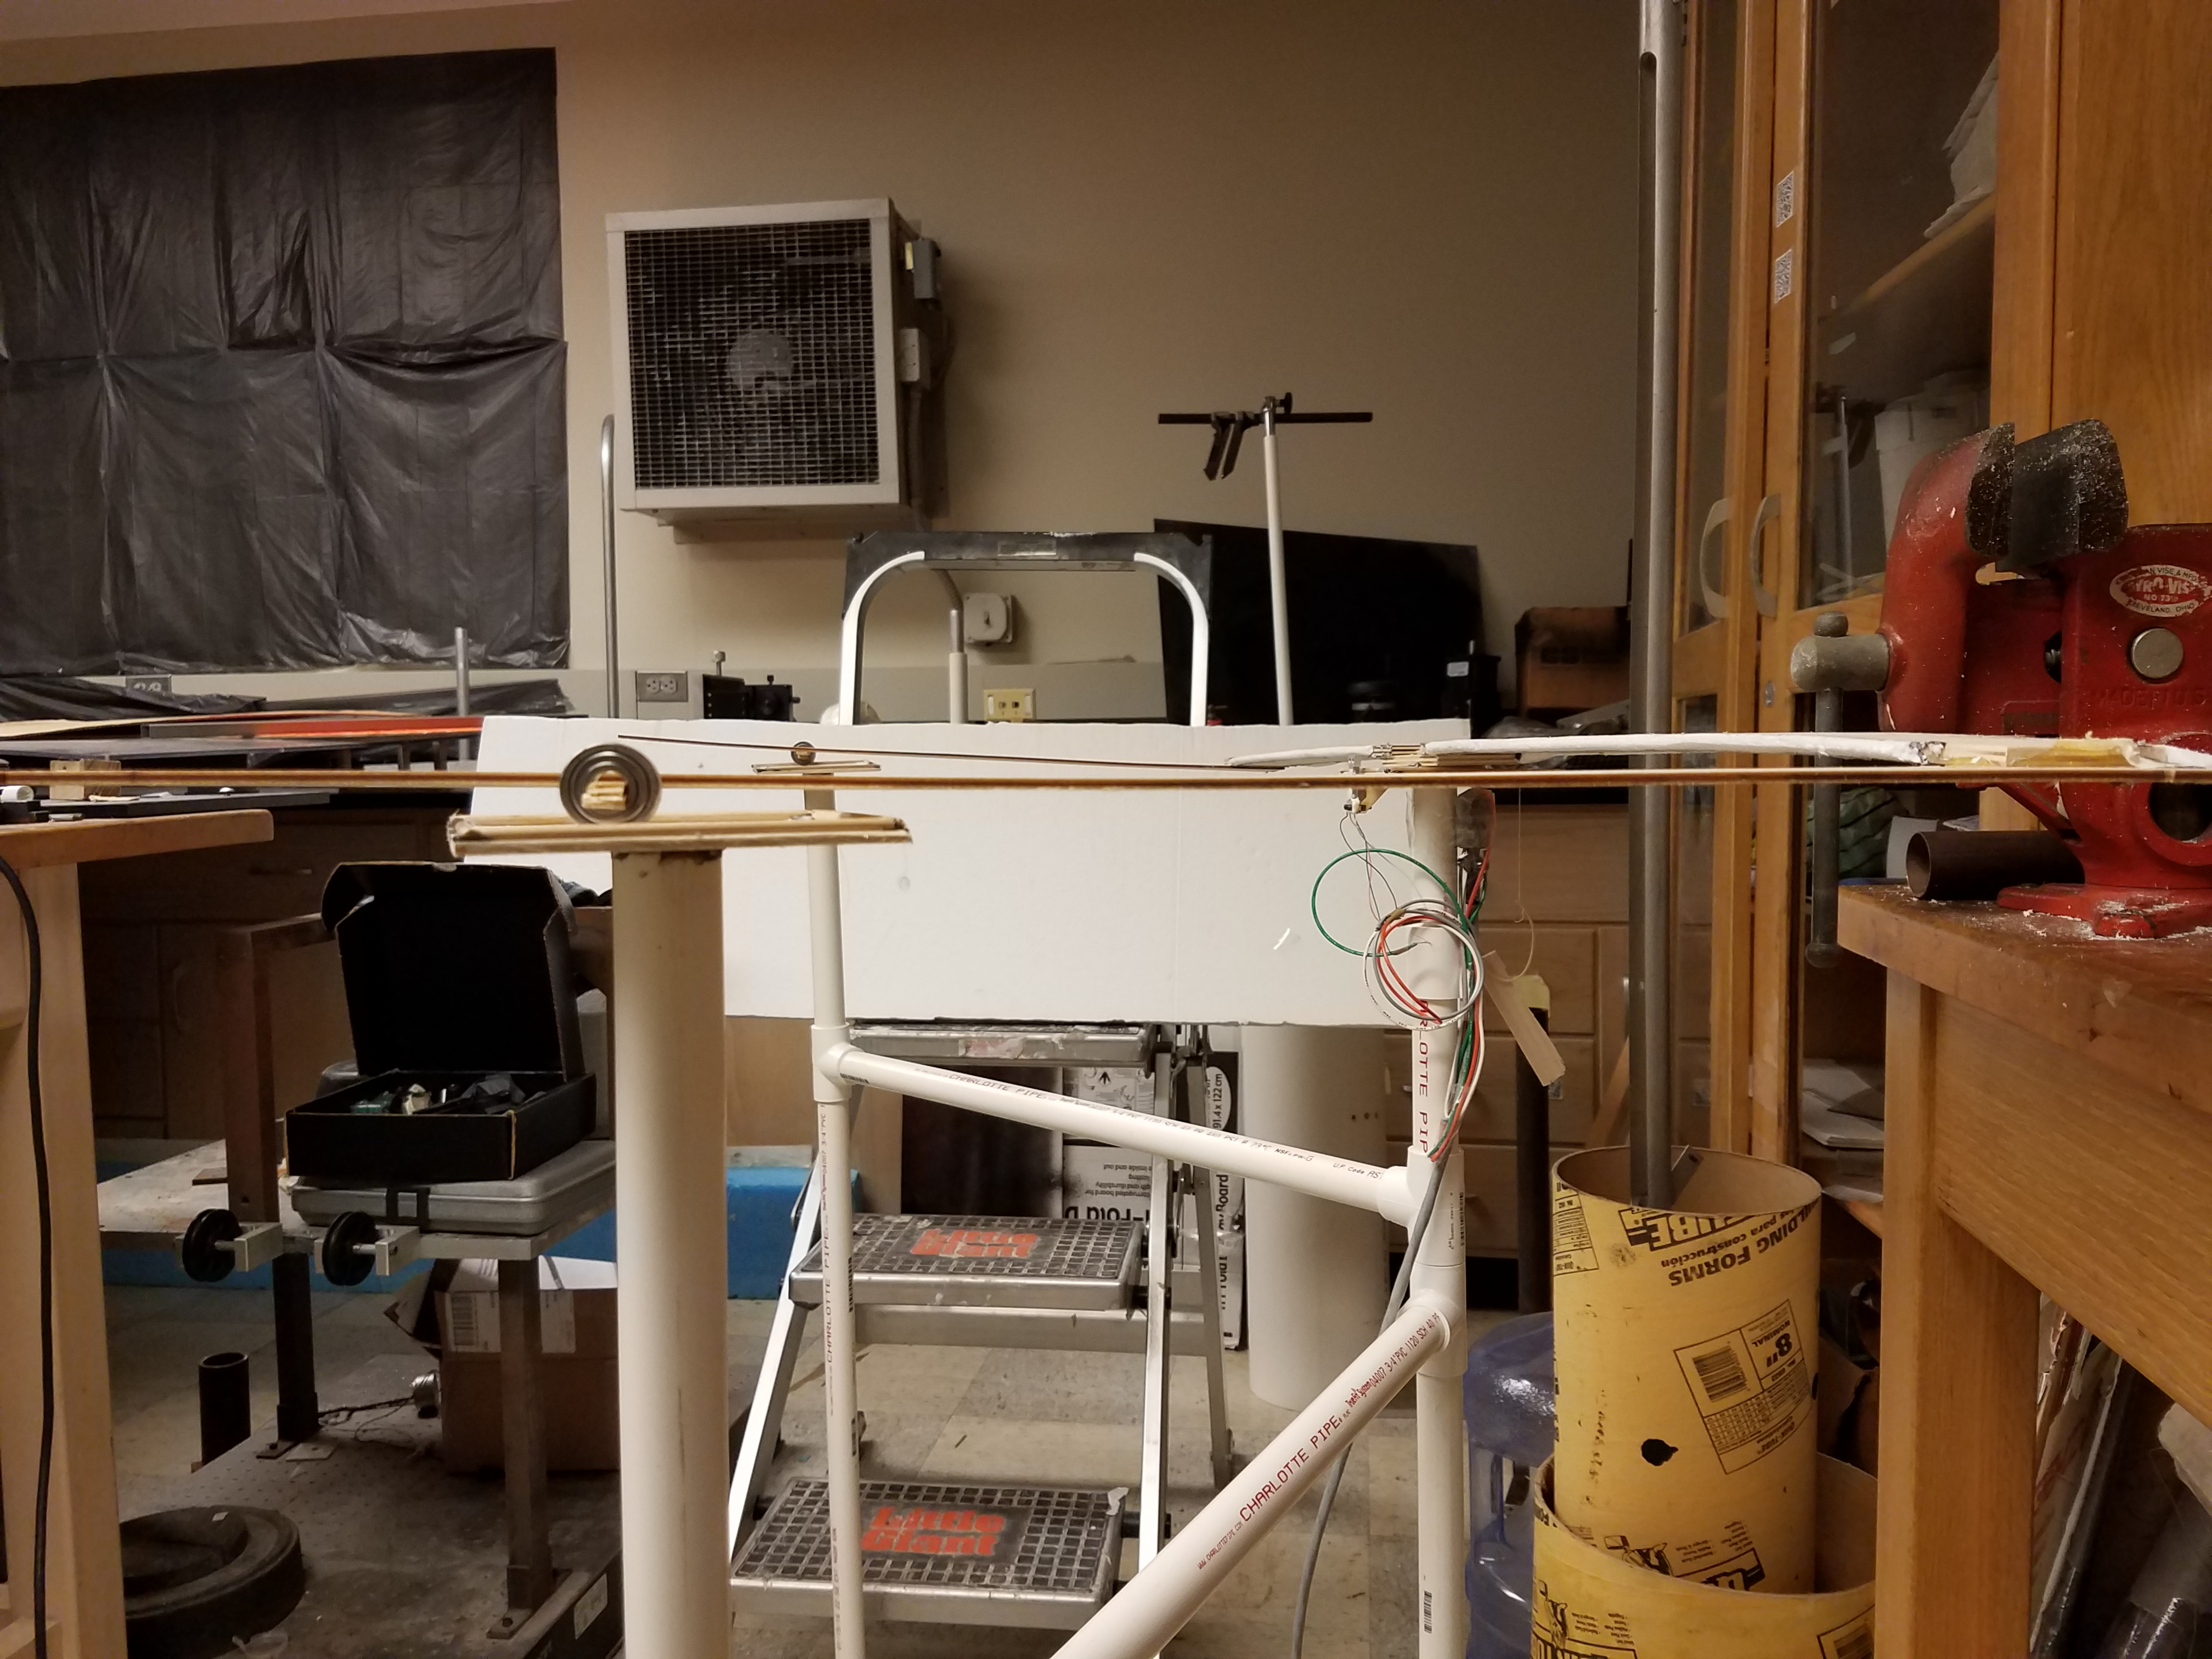
\includegraphics[width = 0.7\linewidth]{skewness.jpg}
\centering
\caption{Without corrective measures, the right (starboard) side of the sheet frame is at a higher angle than the left.}
\label{skewness}
\end{figure}

\begin{figure}
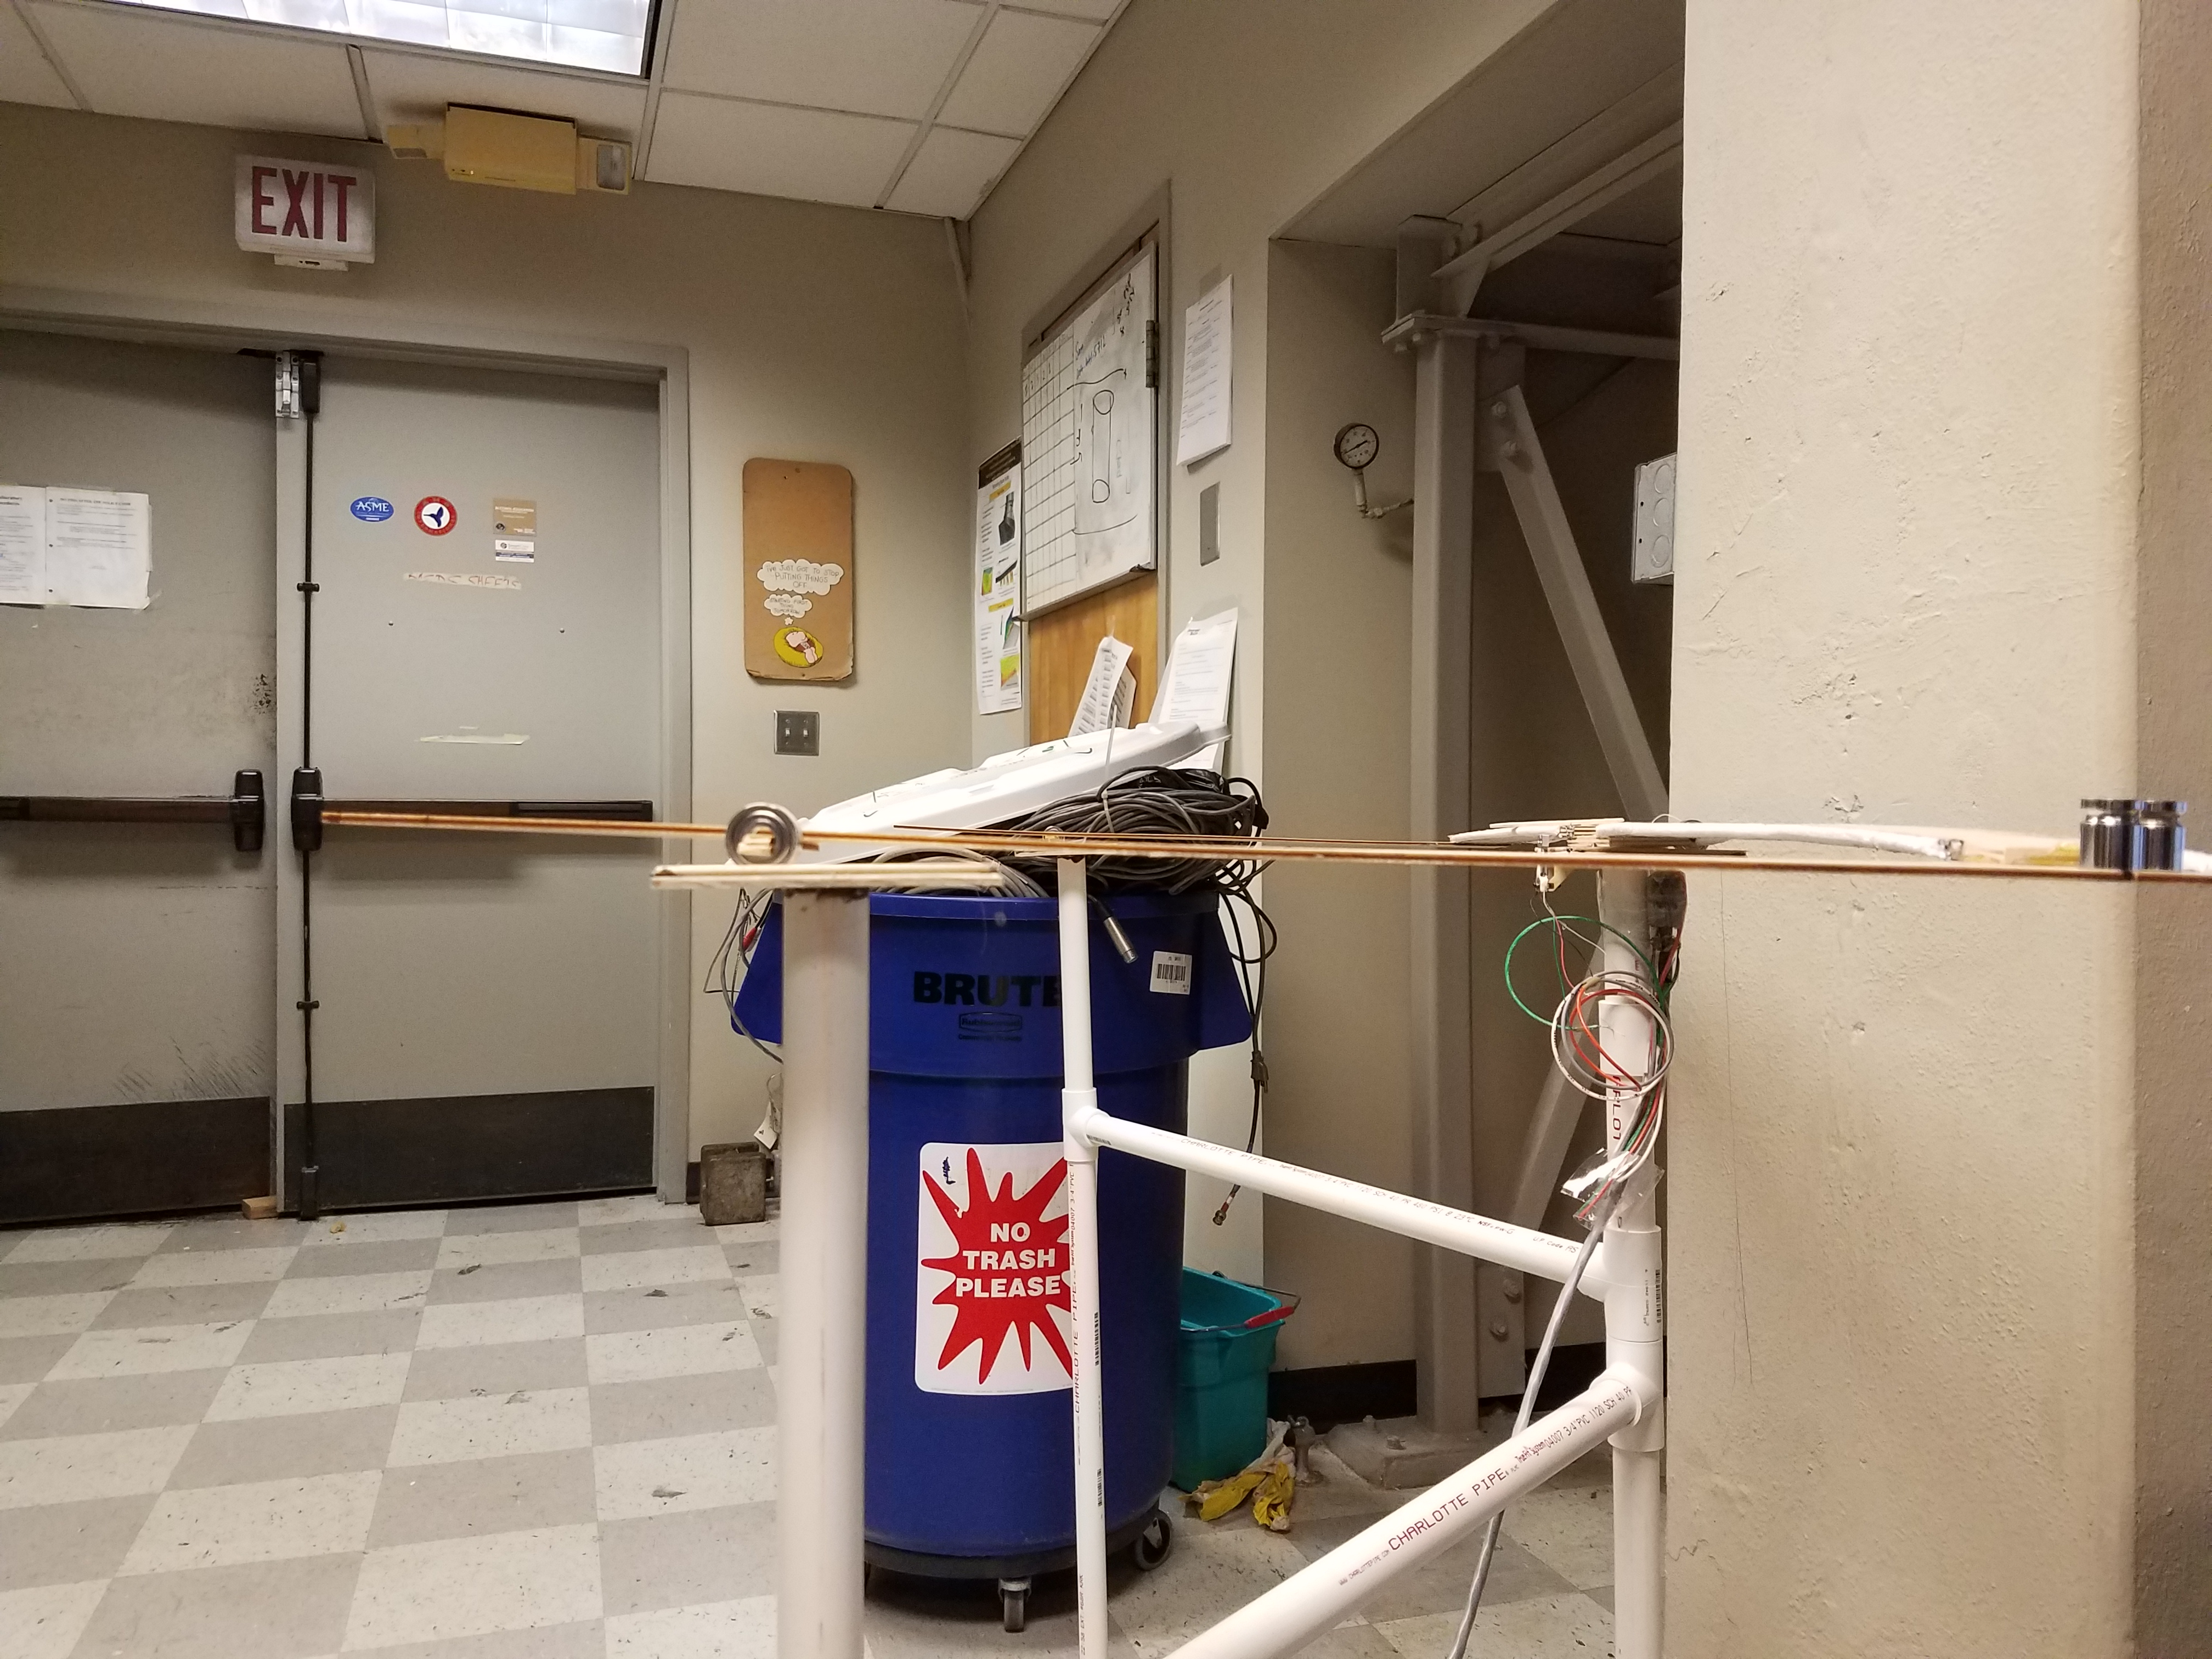
\includegraphics[width = 0.7\linewidth]{skewness_correction.jpg}
\centering
\caption{Correcting the twist of the sheet frame by adding weight to the left (port) side.}
\label{skewness_correction}
\end{figure}

\subsubsection{Second Iteration}
The idea behind the second iteration is to eliminate the drag of the support structure by enclosing it. Essentially, we take
what we had before and put a shell around it which keeps it out of the flow, so that the drag is negligible. Figure
\ref{second_iteration_schematic} illustrates this concept. The sheet is still connected to the frame by means of wires, which
run through small holes in the shell. Care must be taken to ensure that the shell does not touch the wires, to prevent error
in the measurements. The frame still has bearings, but instead of rolling on three separate surfaces, it rolls inside the
shell. The shell is connected directly to the PVC pipe support structure. Then, load cell is mounted to the shell, and is
still connected
to the frame by a thread. Therefore, the shell transfers its own drag force to the PVC pipes, whereas
the frame recieves all of the drag force of the sheet and transfers all of it to the load cell, minus the friction in the
bearings. Since there must necessarily be a few holes in the shell, the force on the frame will not be exactly zero, but
it should be small compared to the drag on the sheet.

\begin{figure}
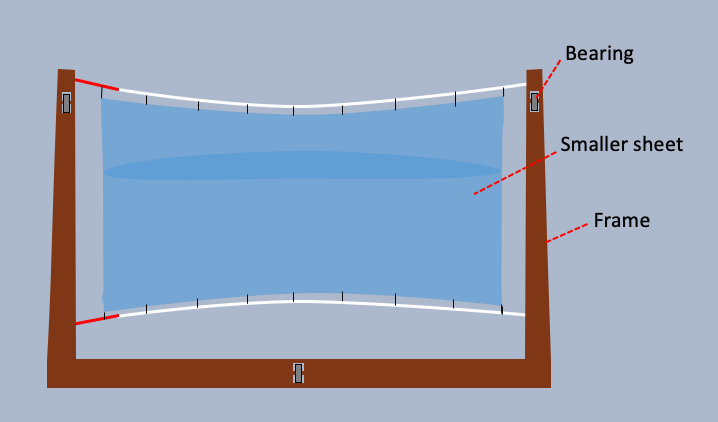
\includegraphics[width = \linewidth]{zero_inside.png}
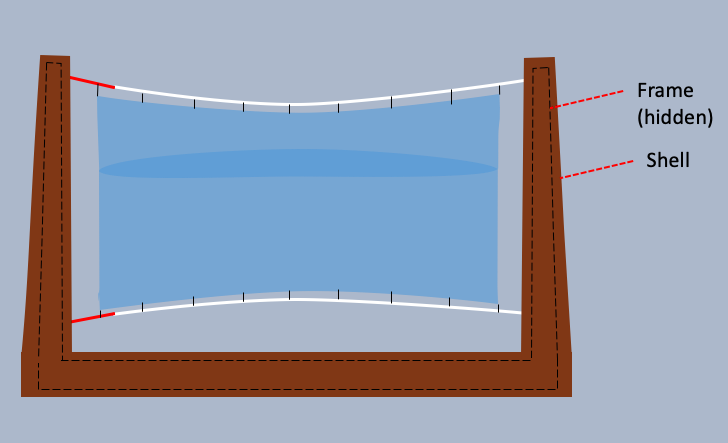
\includegraphics[width = \linewidth]{zero_outside.png}
\centering
\caption{Schematic representation of the second iteration.}
\label{second_iteration_schematic}
\end{figure}

The existence of the shell also solves another problem. Before, the tests could not be run at high speed out of concern
that the model might lift off of the PVC pipe support structure. The shell prevents the frame from moving up or down,
so this is no longer a concern. Therefore, not only does the shell minimize the error due to extra drag, but it also allows
the tests to be run at high speed, so that the drag of the sheet can be resolved more accurately.

The shell does raise once concern which was less of an issue for the first iteration. Namely, the shell has much more volume
than the frame of the first iteration. While this does not cause problematic drag, it disturbs the flow around the sheet.
Therefore, the sheet in the second iteration must be smaller than the sheet in the first iteration.

In further support of the second iteration, first iteration had problems because of the flexibility of the frame. After
construction of the first iteration, the entire structure was twisted, which would cause one side of the sheet to be at higher
angle of attack than the other. This was mitigated by adding weights to one side of the structure, but it would be advantageous
if the twist were not present in the first place. Furthermore, the frame deformed slightly when the wires were added, and
flutter was observed during testing. The flexibility occurred because the frame was designed to be as thin as possible, which
required the structural design to be compromised. However, since the second iteration is shielded from the flow and produces
little drag, it may be made much stiffer.

The second-iteration frame is made of 3mm thick plywood. It possesses the same general architecture as the first iteration,
but its cross section is box instead of a single sheet. This gives it much greater torsional rigidity, and good bending
rigidity in both axes, instead of only one. Each segment is made of four sheets which are fitted together with alternating
tabs, which allows the plywood itself to take as much any loads as possible, and rely on the adhesive less. The spanwise
segment is split into two pieces, so that it may have twice the length of the plywood sheets from which it is made. The two
pieces are connected by taps that extend from one into the other. The CAD for
the frame is shown in Figure \ref{insideCAD}.

\begin{figure}
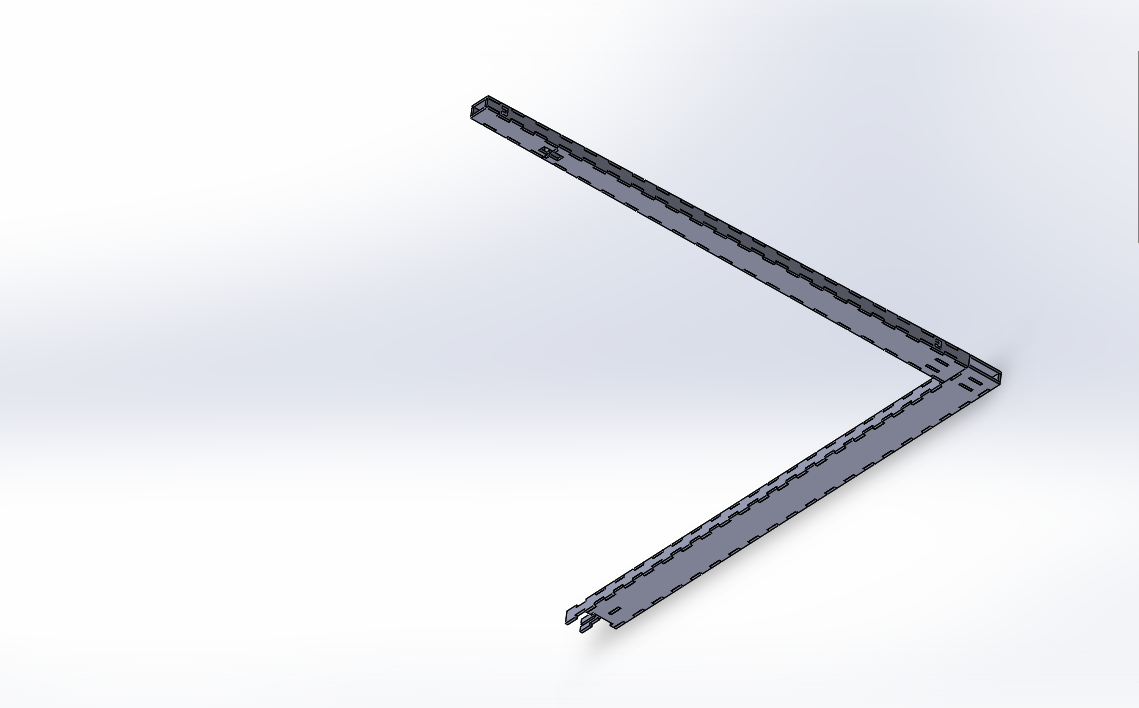
\includegraphics[width = 0.7\linewidth]{insideCAD.png}
\centering
\caption{The CAD model for the second-iteration frame. Only half is shown so that the attachment between the halves
is more clear.}
\label{insideCAD}
\end{figure}

The shell is designed similarly to the frame, except for three things. First, it is bigger, so that the sheet can fit inside of it.
Second, it all tabs which connect the various segments are on the outside rather than the inside, since the frame must occupy the
inside without obstructions. Third, only three faces of every segment are made of plywood. Thus, it may be constructed with missing
faces, and the frame may be inserted and accessed through those faces. After the frame has been inserted and properly adjusted, the
missing faces may be covered up with a more temporary material (such as tape or cardboard). The CAD for the shell is displayed
in Figure \ref{outsideCAD}.

\begin{figure}
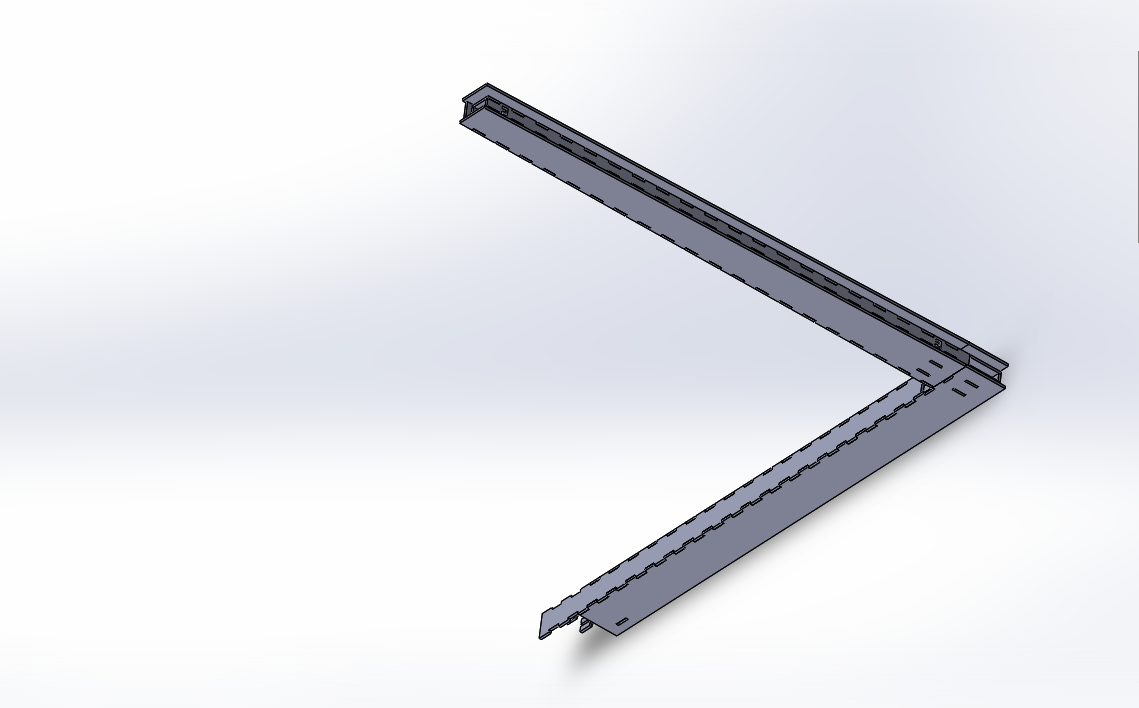
\includegraphics[width = 0.7\linewidth]{outsideCAD.png}
\centering
\caption{The CAD model for the second-iteration setup, including the frame and the shell.}
\label{outsideCAD}
\end{figure}

The plywood components for the second-iteration drag balance are made by laser cutting 3mm thick plywood. These components (shown
in Figure \ref{parts}) were assembled using super glue. Due to the particulars of the laser cutting process, all of the cut surfaces
are not perfectly perpendicular to the face of the plywood. Therefore, when each segment of the frame is being constructed, the
sides of the box deviate slightly from perpendicularity. Therefore, there is an interference fit between the last side of the box
and the prior ones. Sometimes, it was necessary to use a knife blade in order to deform the box enough to fit the last side in. This
process is illustrated in Figure \ref{snapping}. This interference fit is actually useful, because the friction decreases the amount
of adhesive which is required to hold the last face to the others. This makes it easier to disassemble and modify if necessary.

\begin{figure}
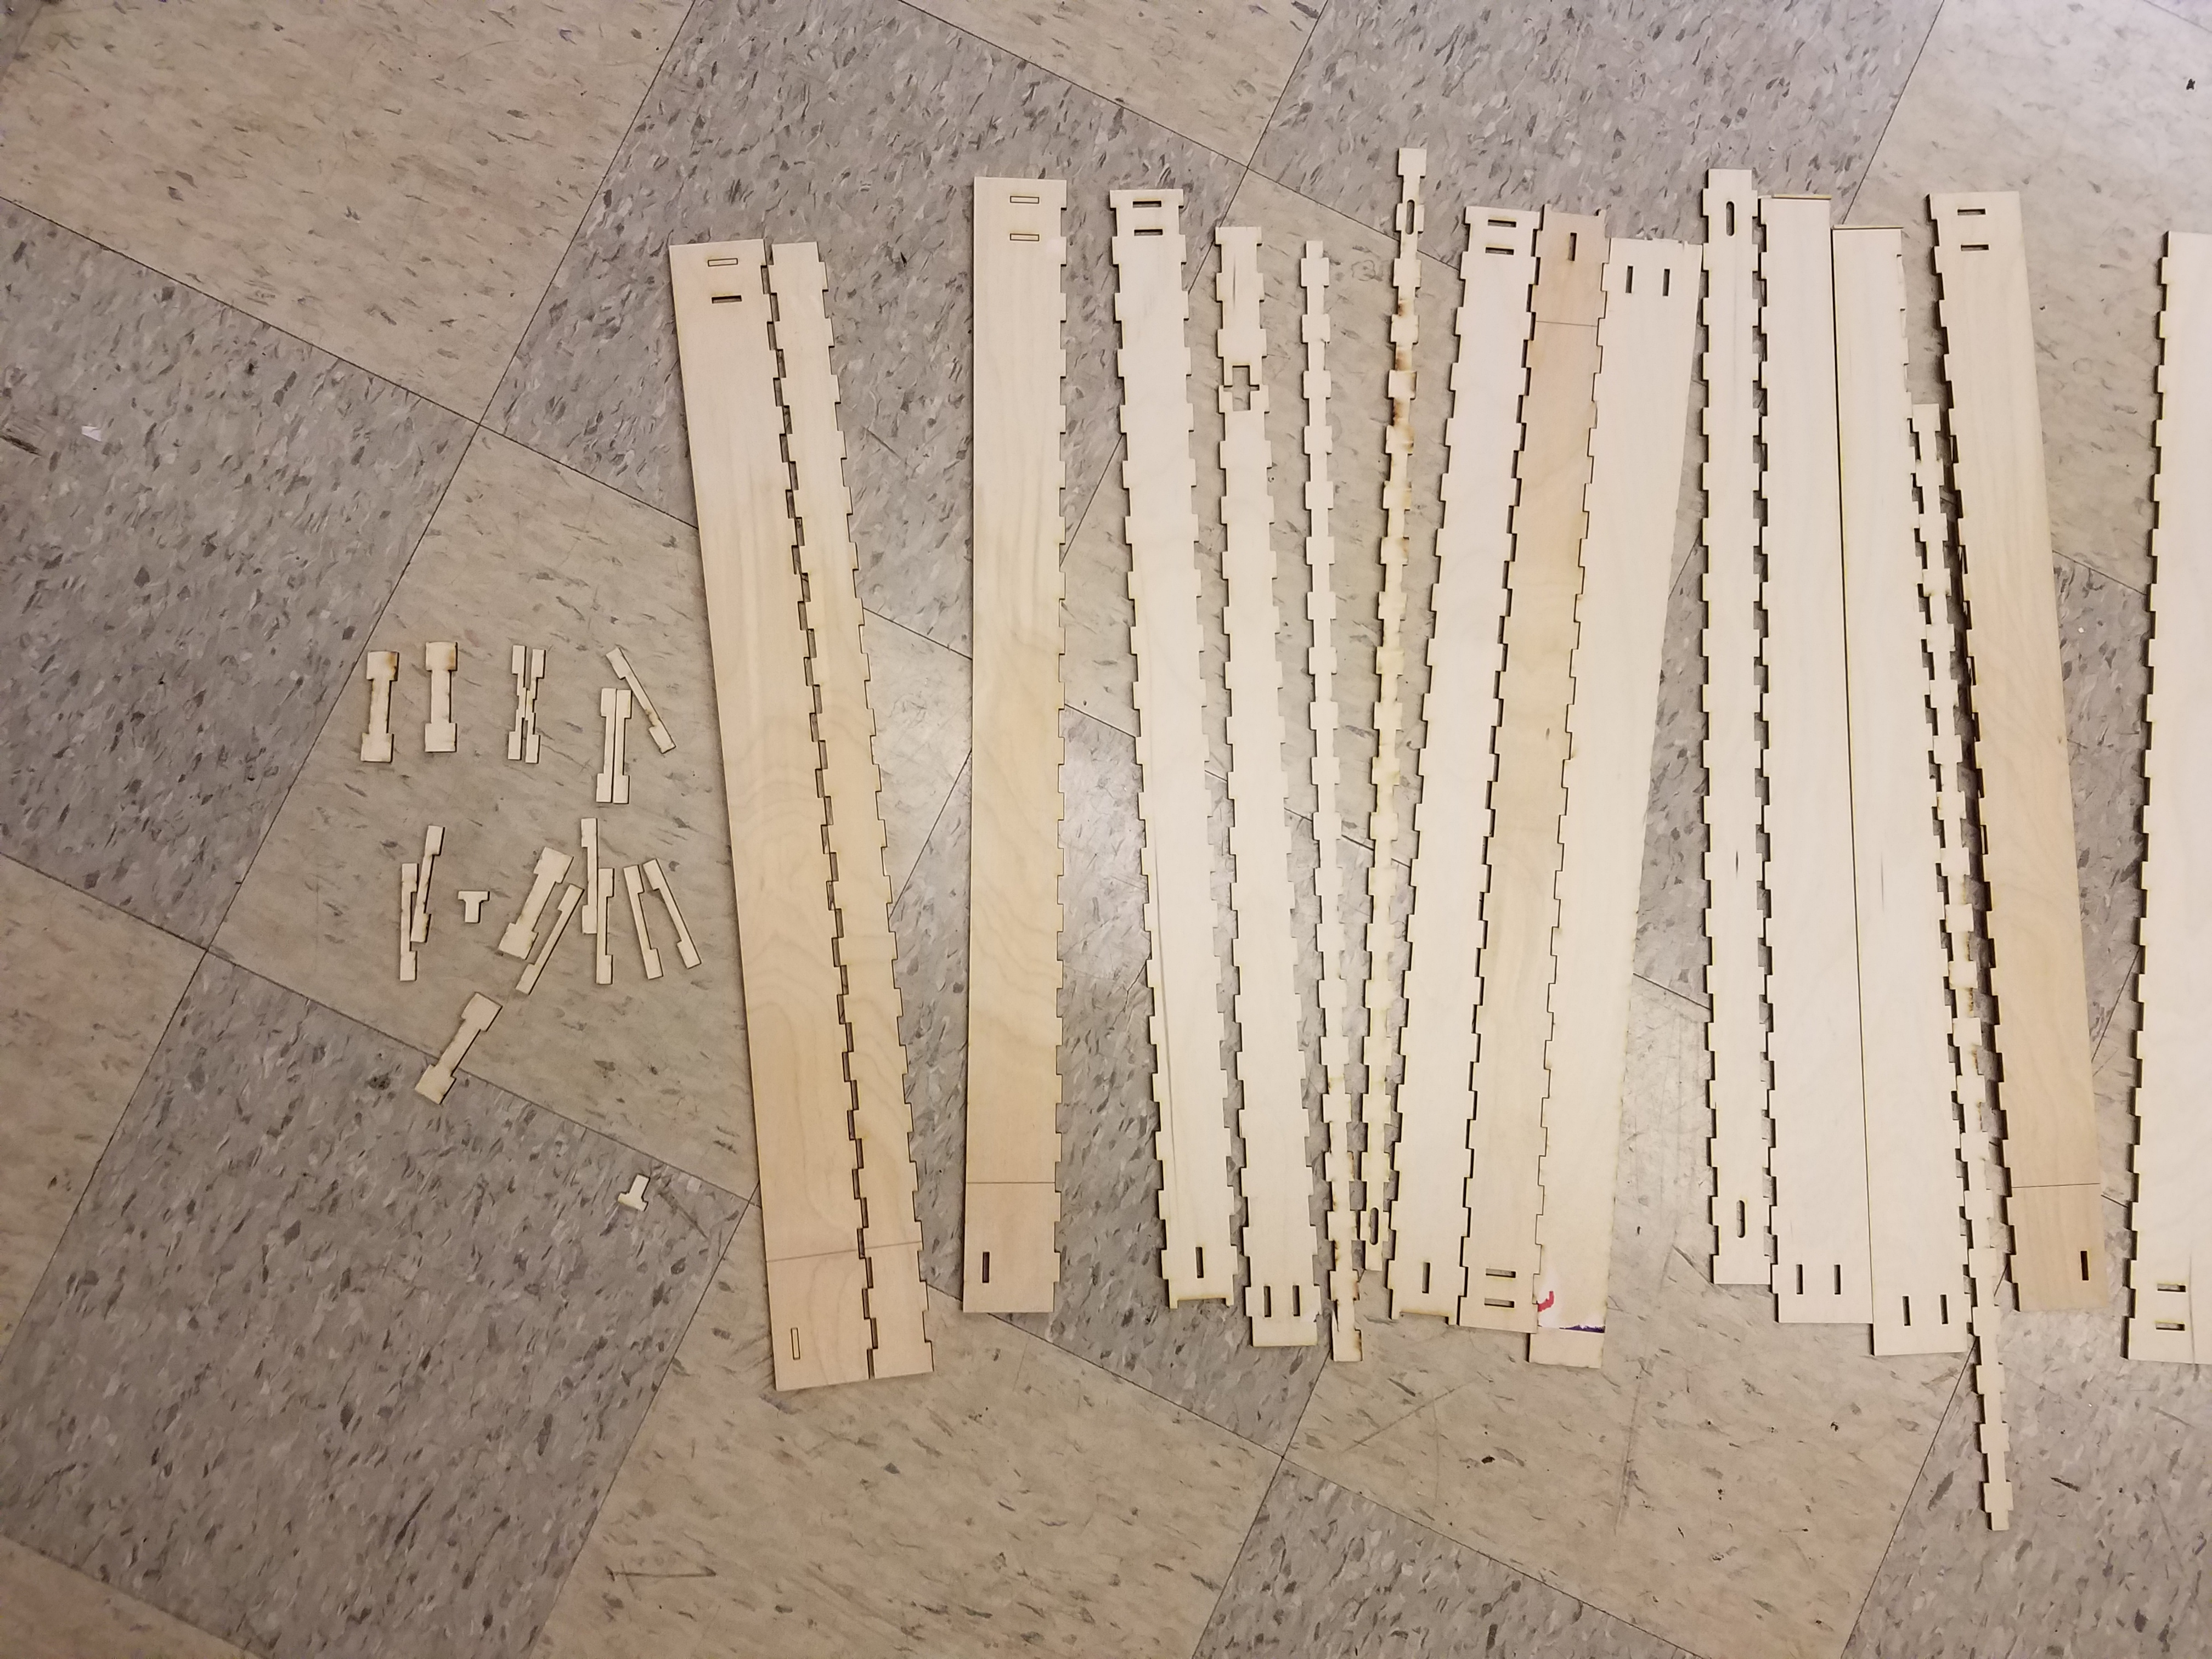
\includegraphics[width = 0.7\linewidth]{parts.jpg}
\centering
\caption{The plywood components for the second iteration drag balance.}
\label{parts}
\end{figure}

\begin{figure}
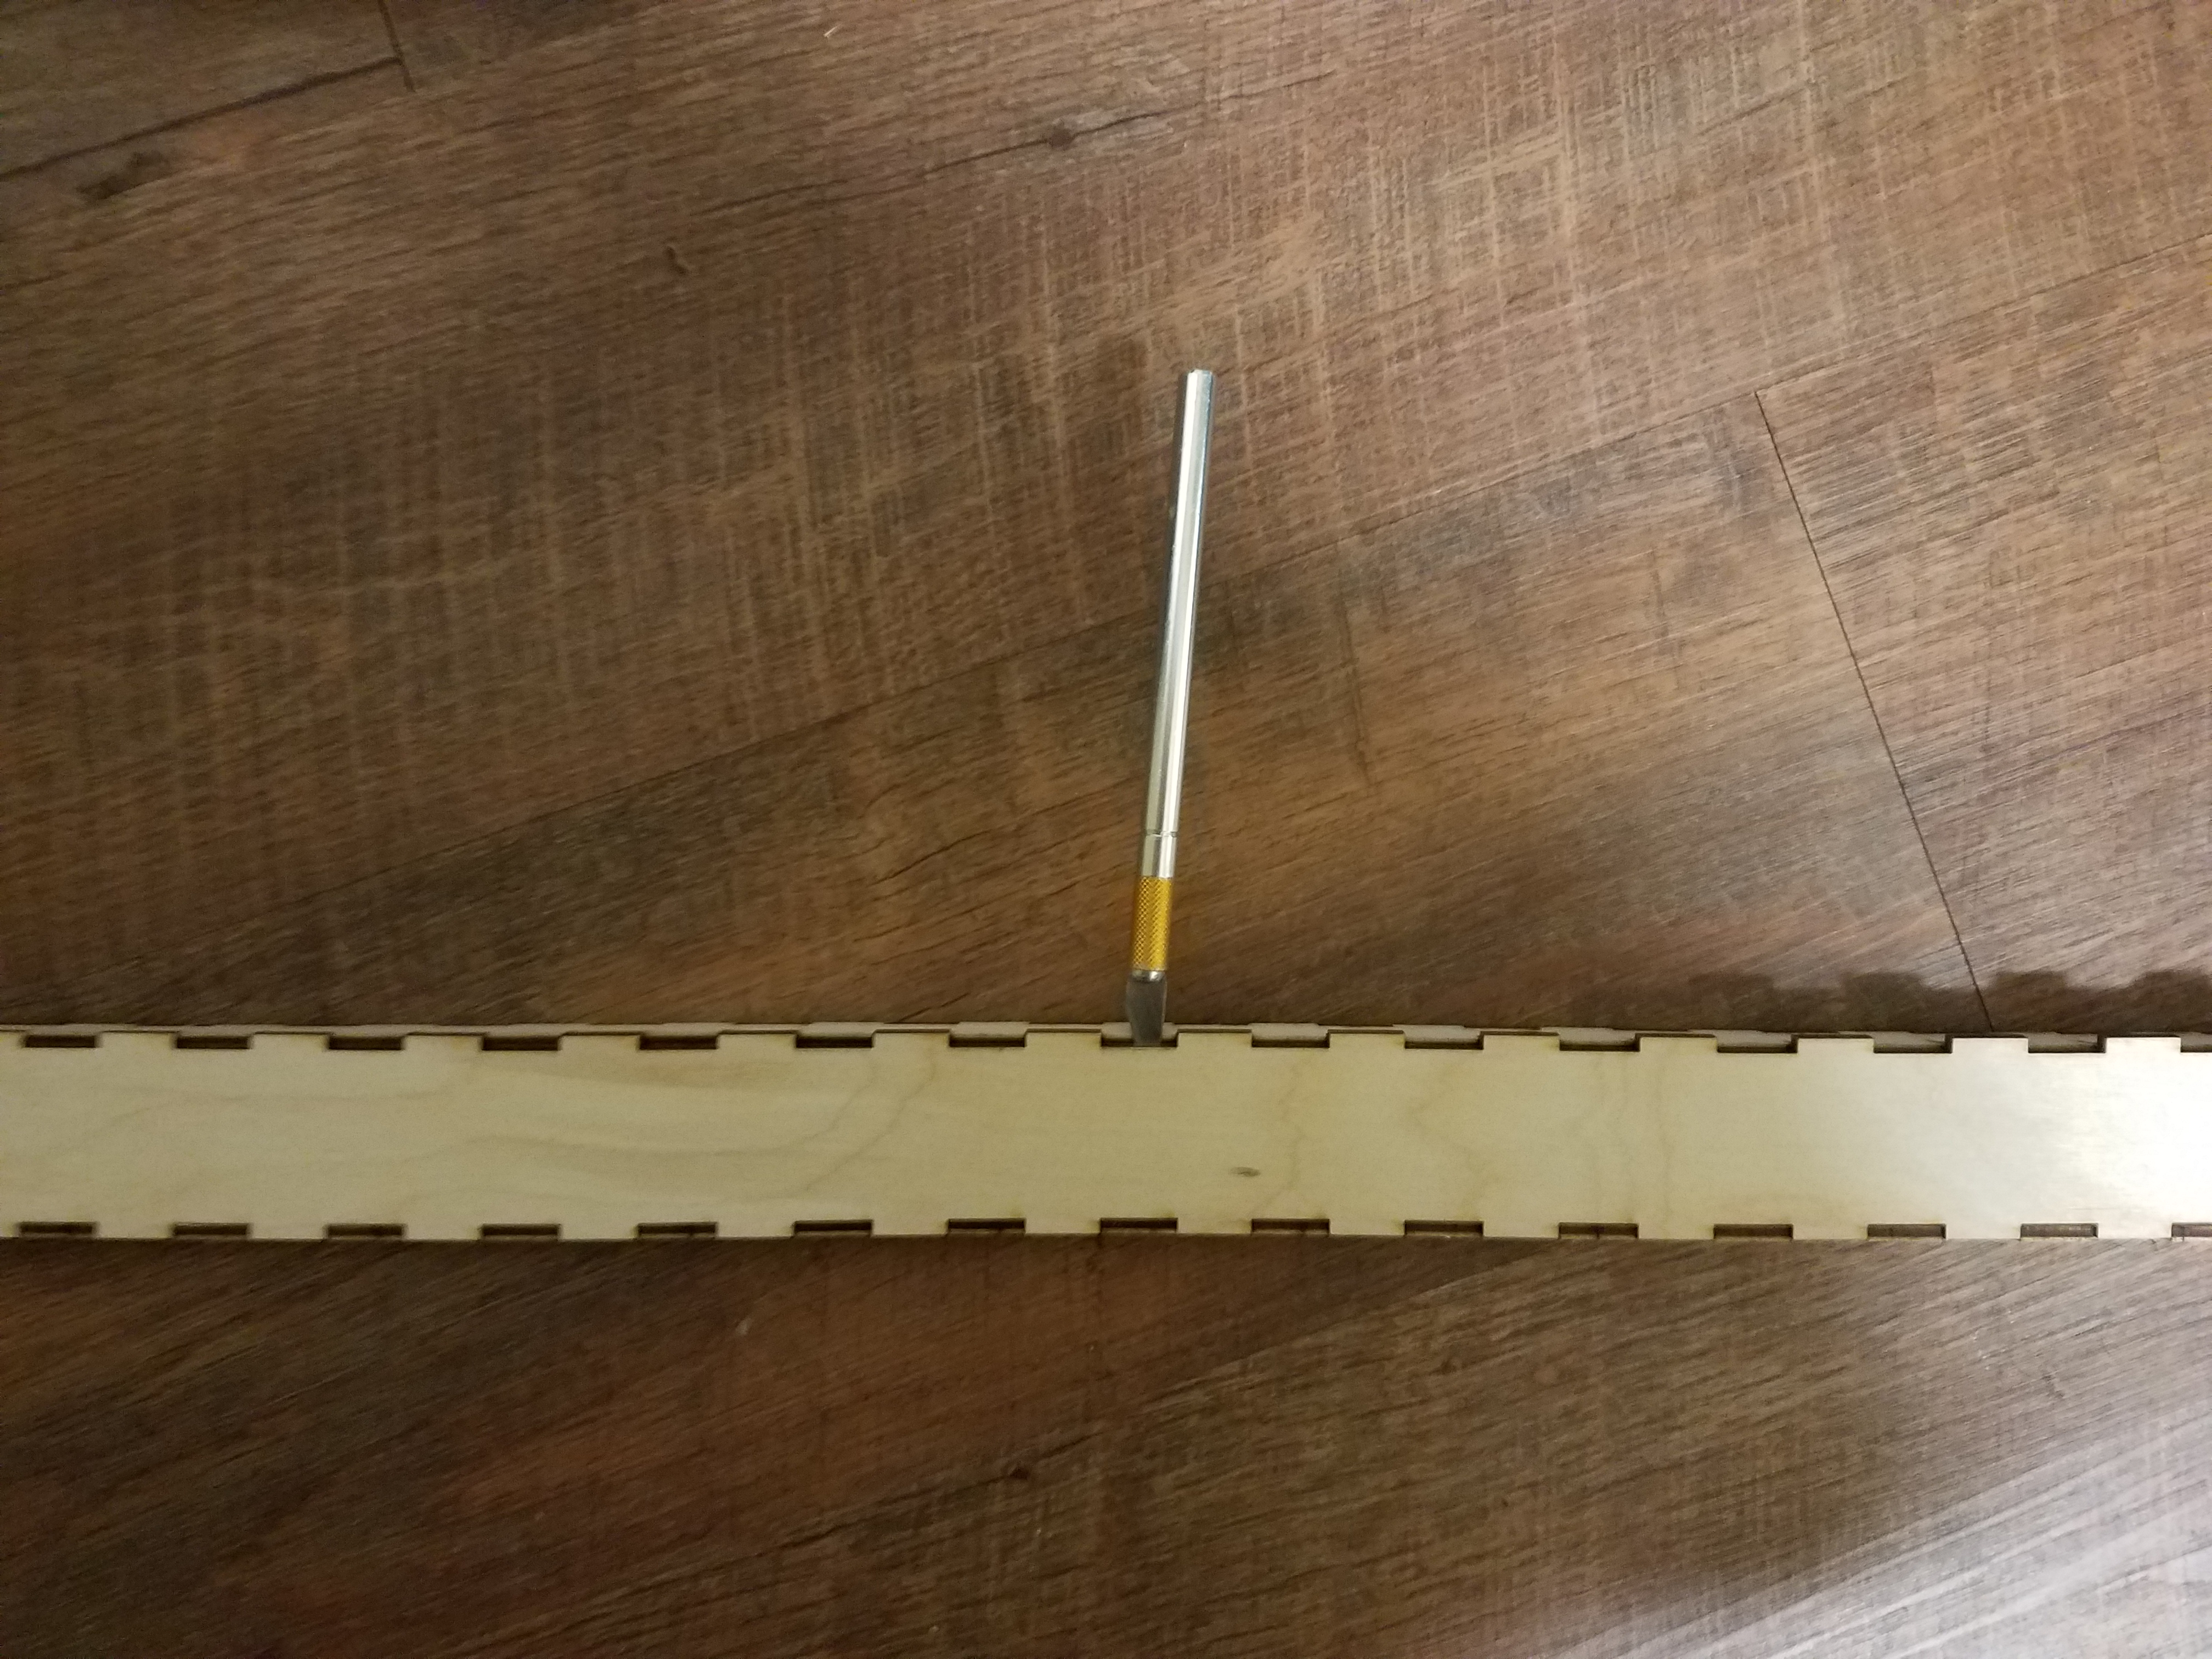
\includegraphics[width = 0.49\linewidth]{snapping1.jpg}
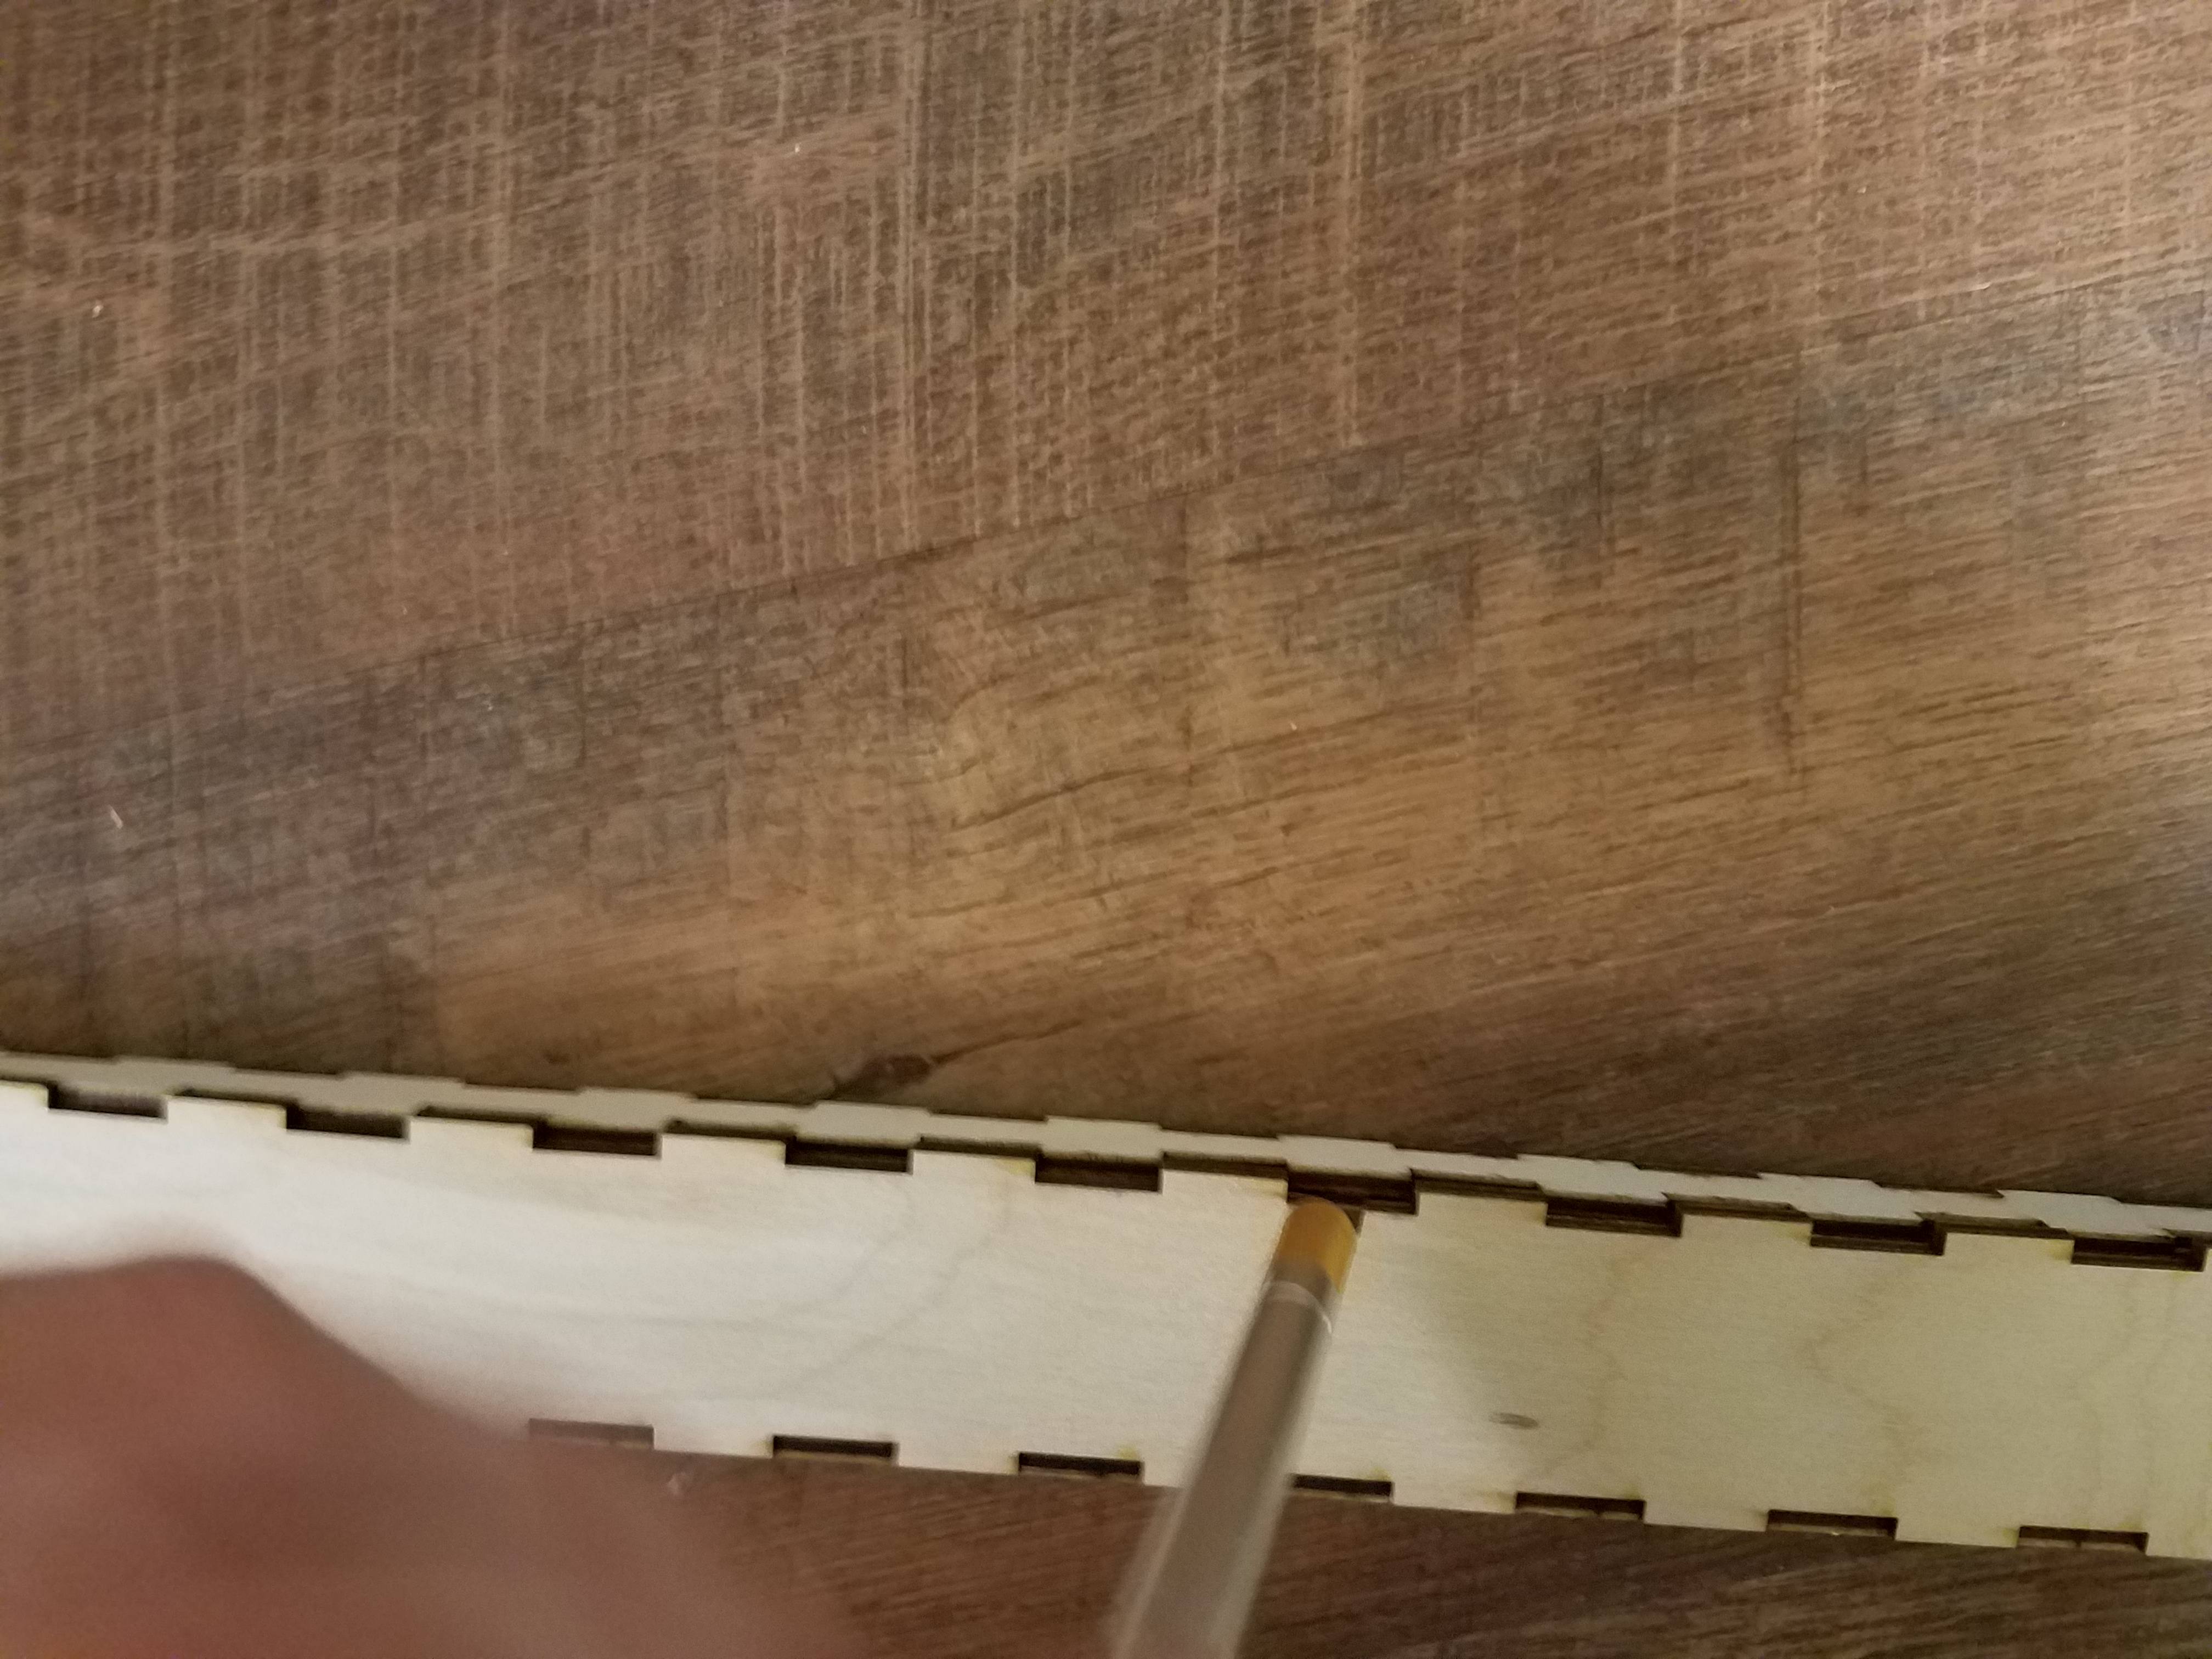
\includegraphics[width = 0.49\linewidth]{snapping2.jpg}
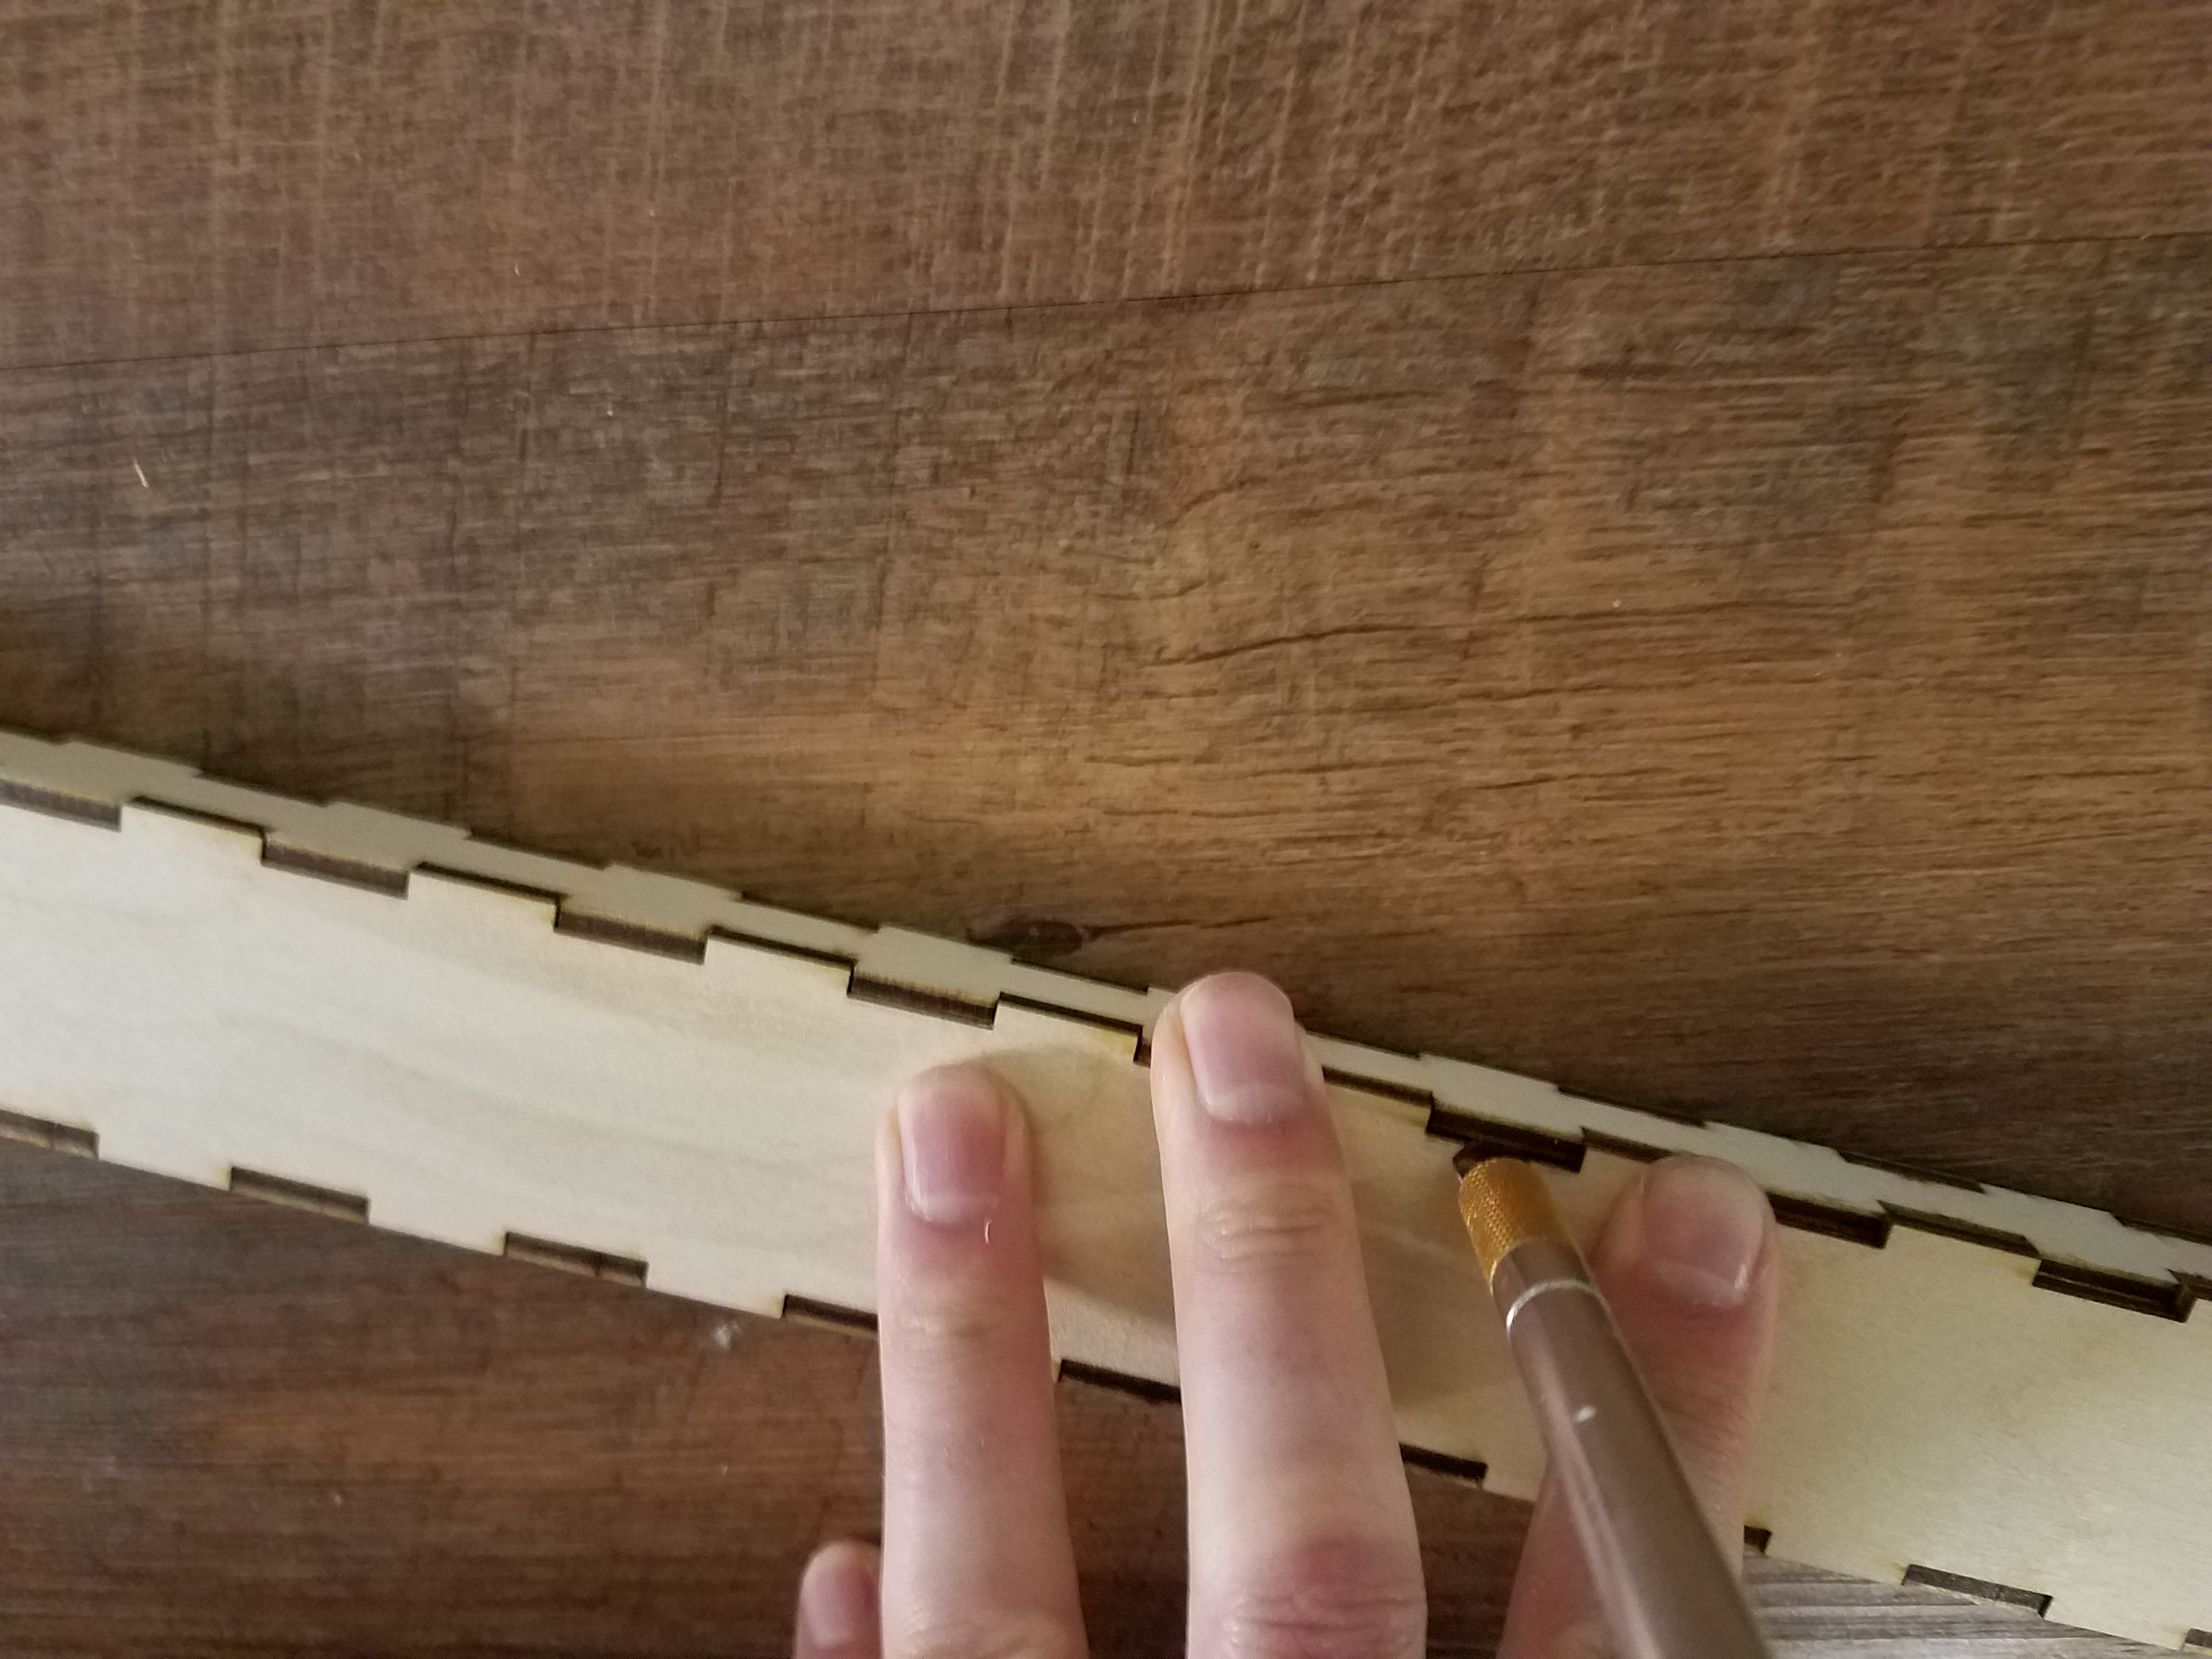
\includegraphics[width = 0.49\linewidth]{snapping3.jpg}
\centering
\caption{Inserting the last face of each segment into an inteference fit.}
\label{snapping}
\end{figure}

When the second iteration had been mostly finished (Figure \ref{shell_finished}), a problem was discovered. Namely, even
though the rigidity has been increased, the corners of the structure bend downward. For one thing, this changes the angle of attack
of one end of the sheet with respect to the other. This problem was more severe on the first iteration, but it has not been eliminated.
However, far more important is that the bending causes the frame structure to touch the shell. This causes substantial friction which
renders the force measurements meaningless. Therefore, a solution to the bending problem is being developed. The bearings have been
eliminated, and the inside frame has been hung inside the shell using threads. Thus, the threads hold the frame up without generating
any streamwise force. This idea has some similarities to the axial force balance.

\begin{figure}
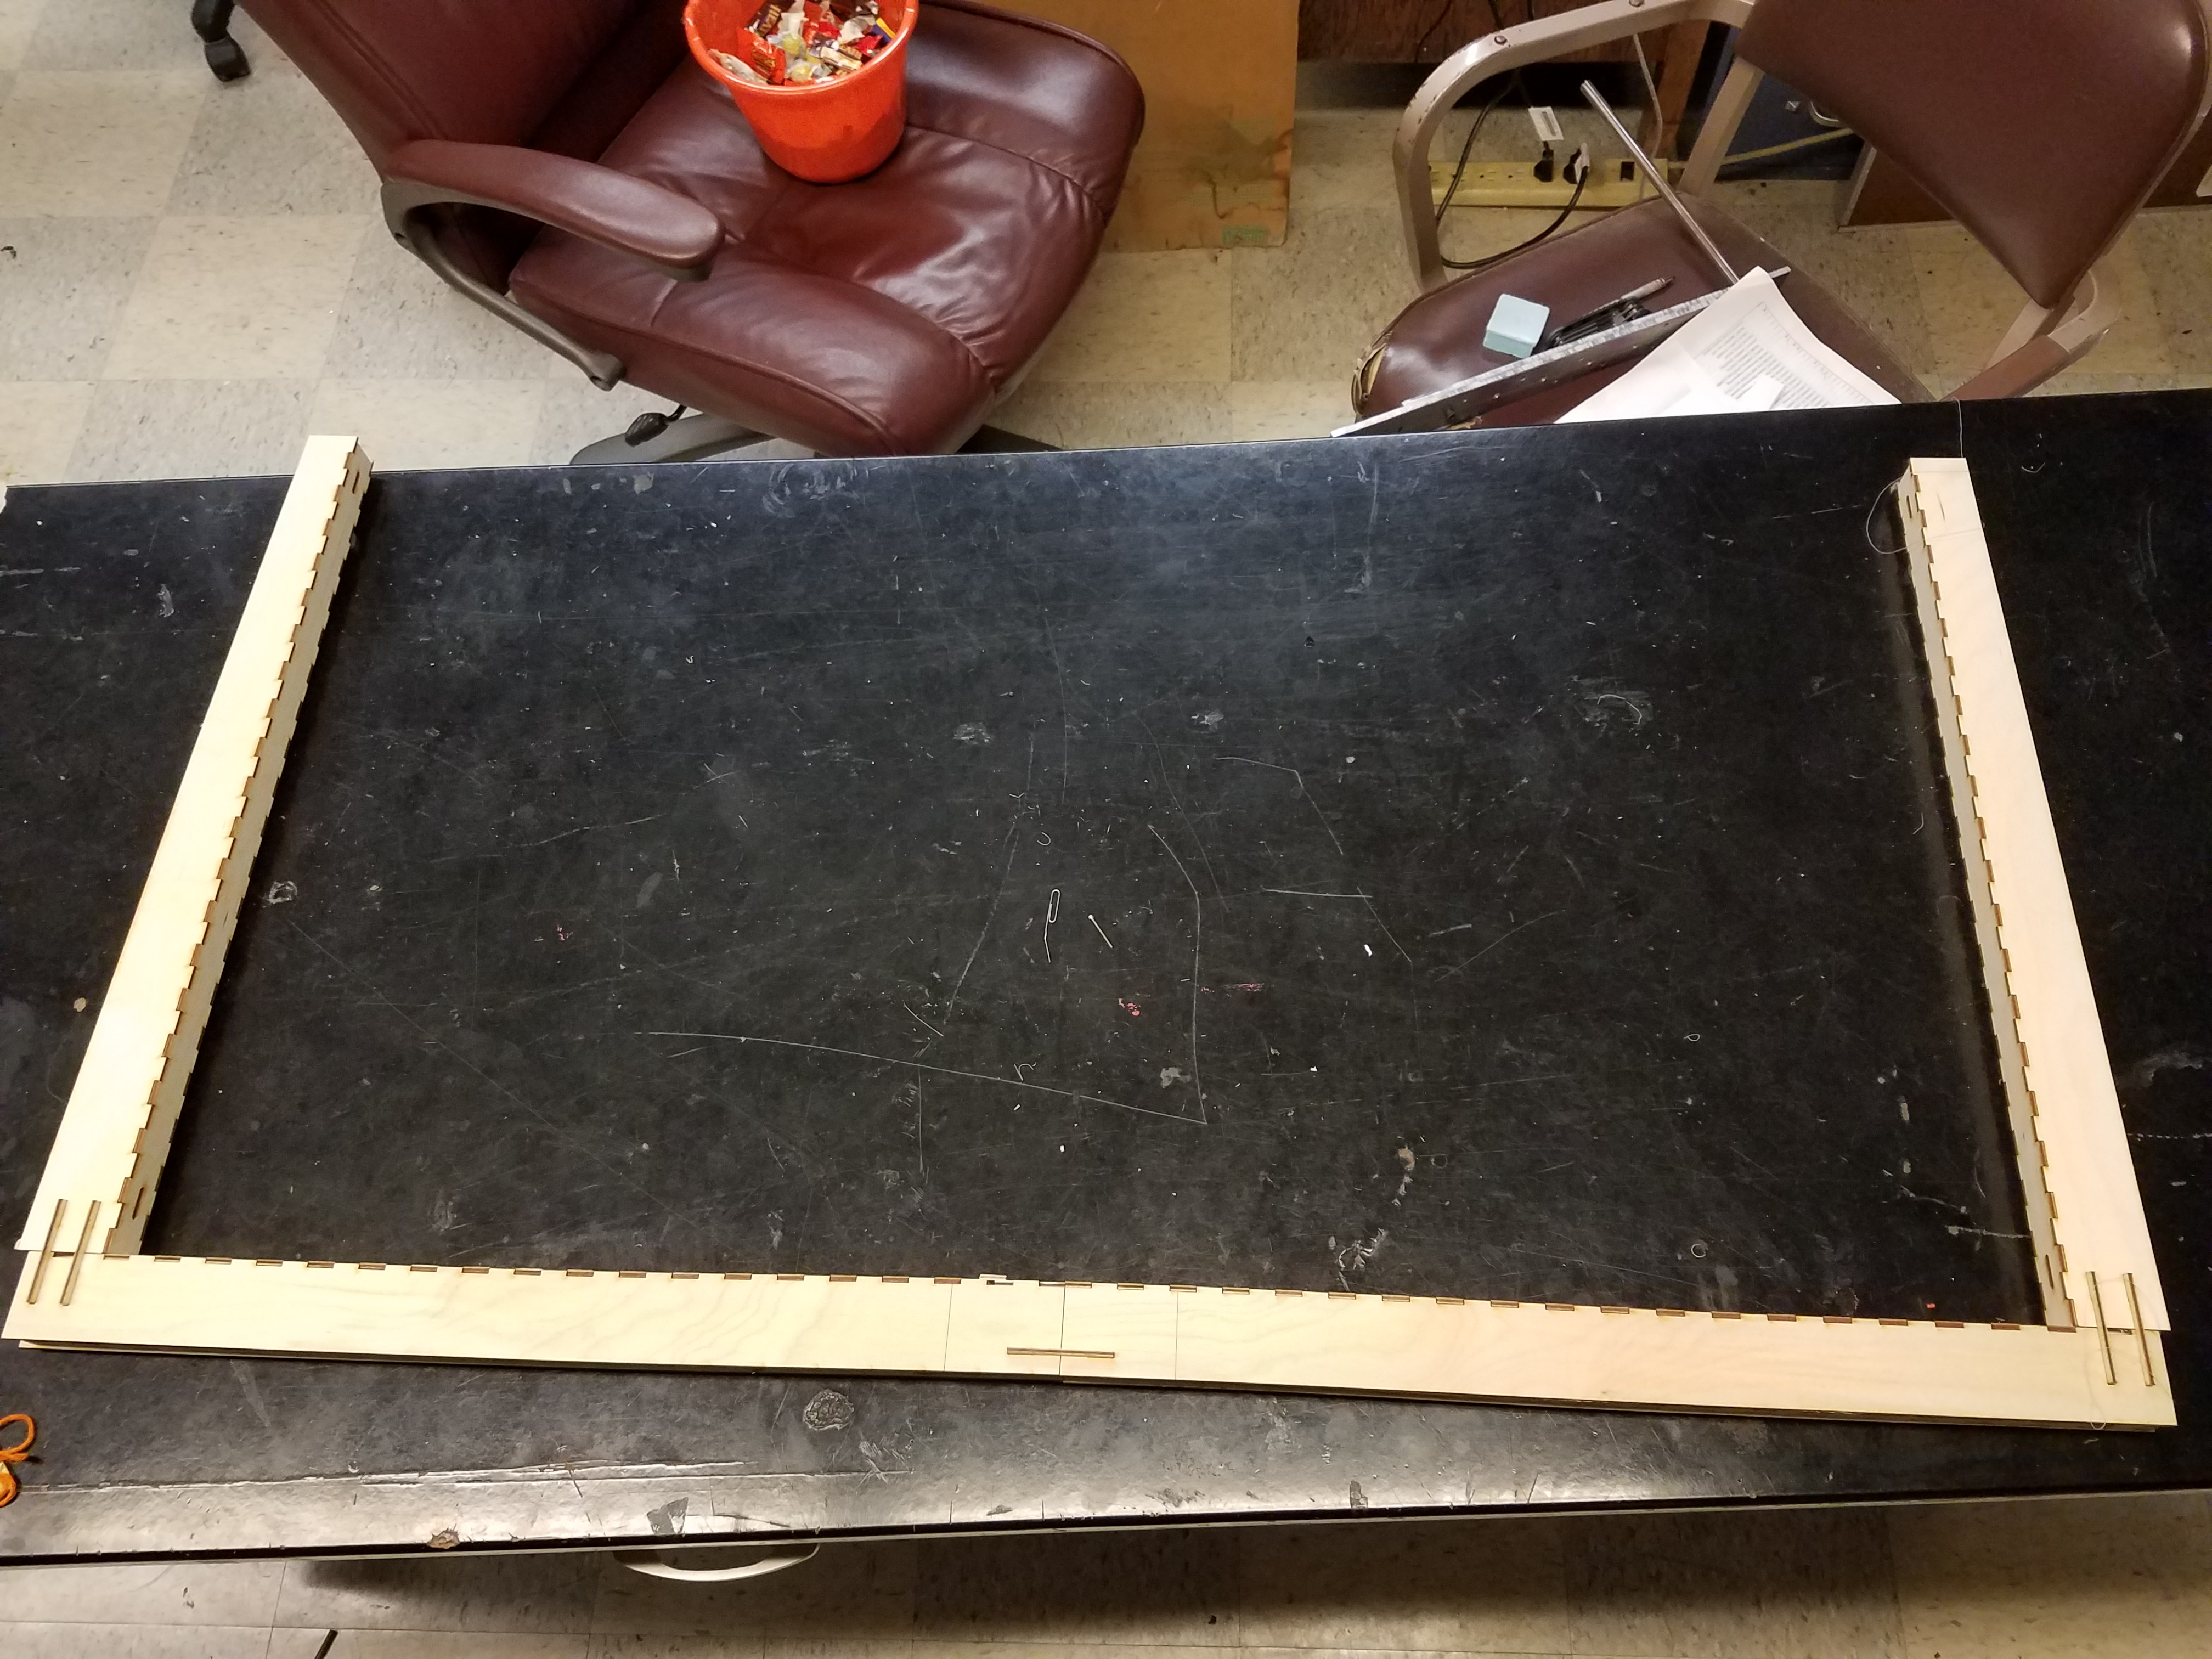
\includegraphics[width = 0.7\linewidth]{shell_finished.jpg}
\centering
\caption{The finished shell that the frame fits inside.}
\label{shell_finished}
\end{figure}

Figure \ref{thread_insertion} shows the threads being installed. First, the frame was placed on top of the shell in the exact
horizontal position it is intended to occupy inside the shell. Then holes were drilled through the frame into the shell. The
threads were drawn through both holes, then pulled tight and secured on each end with cyanoacrylate adhesive. The frame now
hangs inside the shell with a few milimeters of clearance above, below, and on either side

\begin{figure}
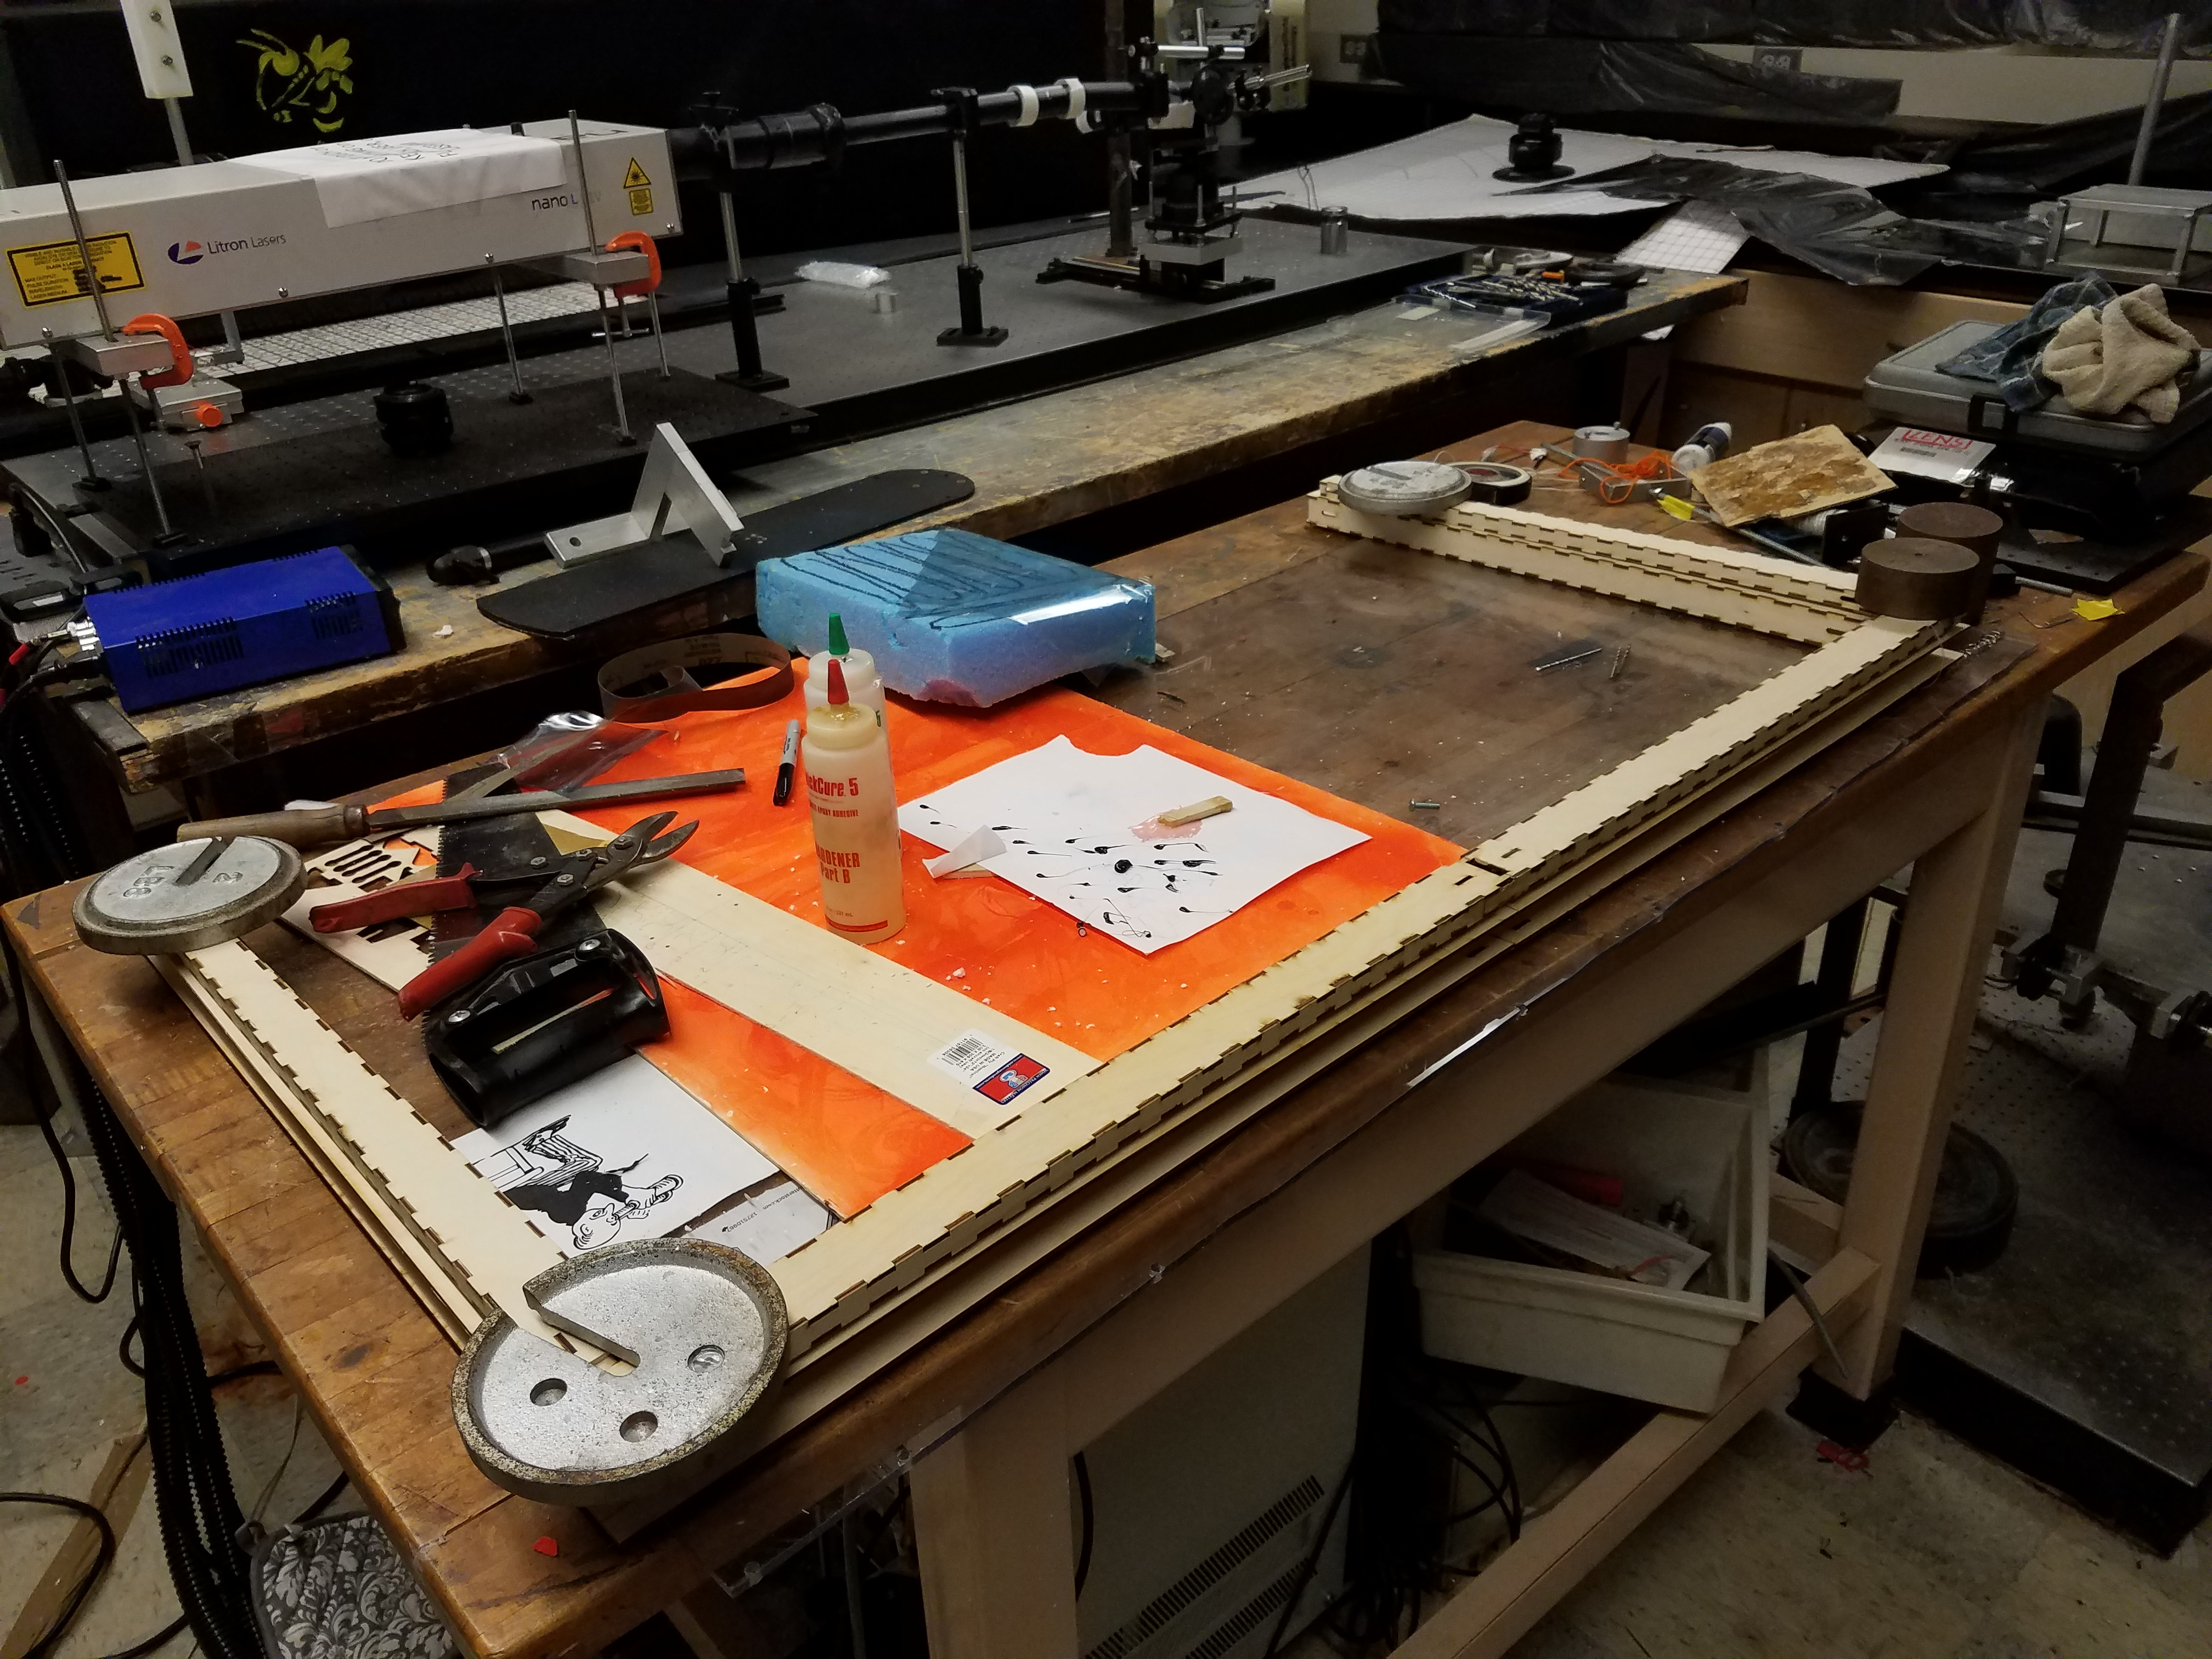
\includegraphics[width = 0.49\linewidth]{threading-1.jpg}
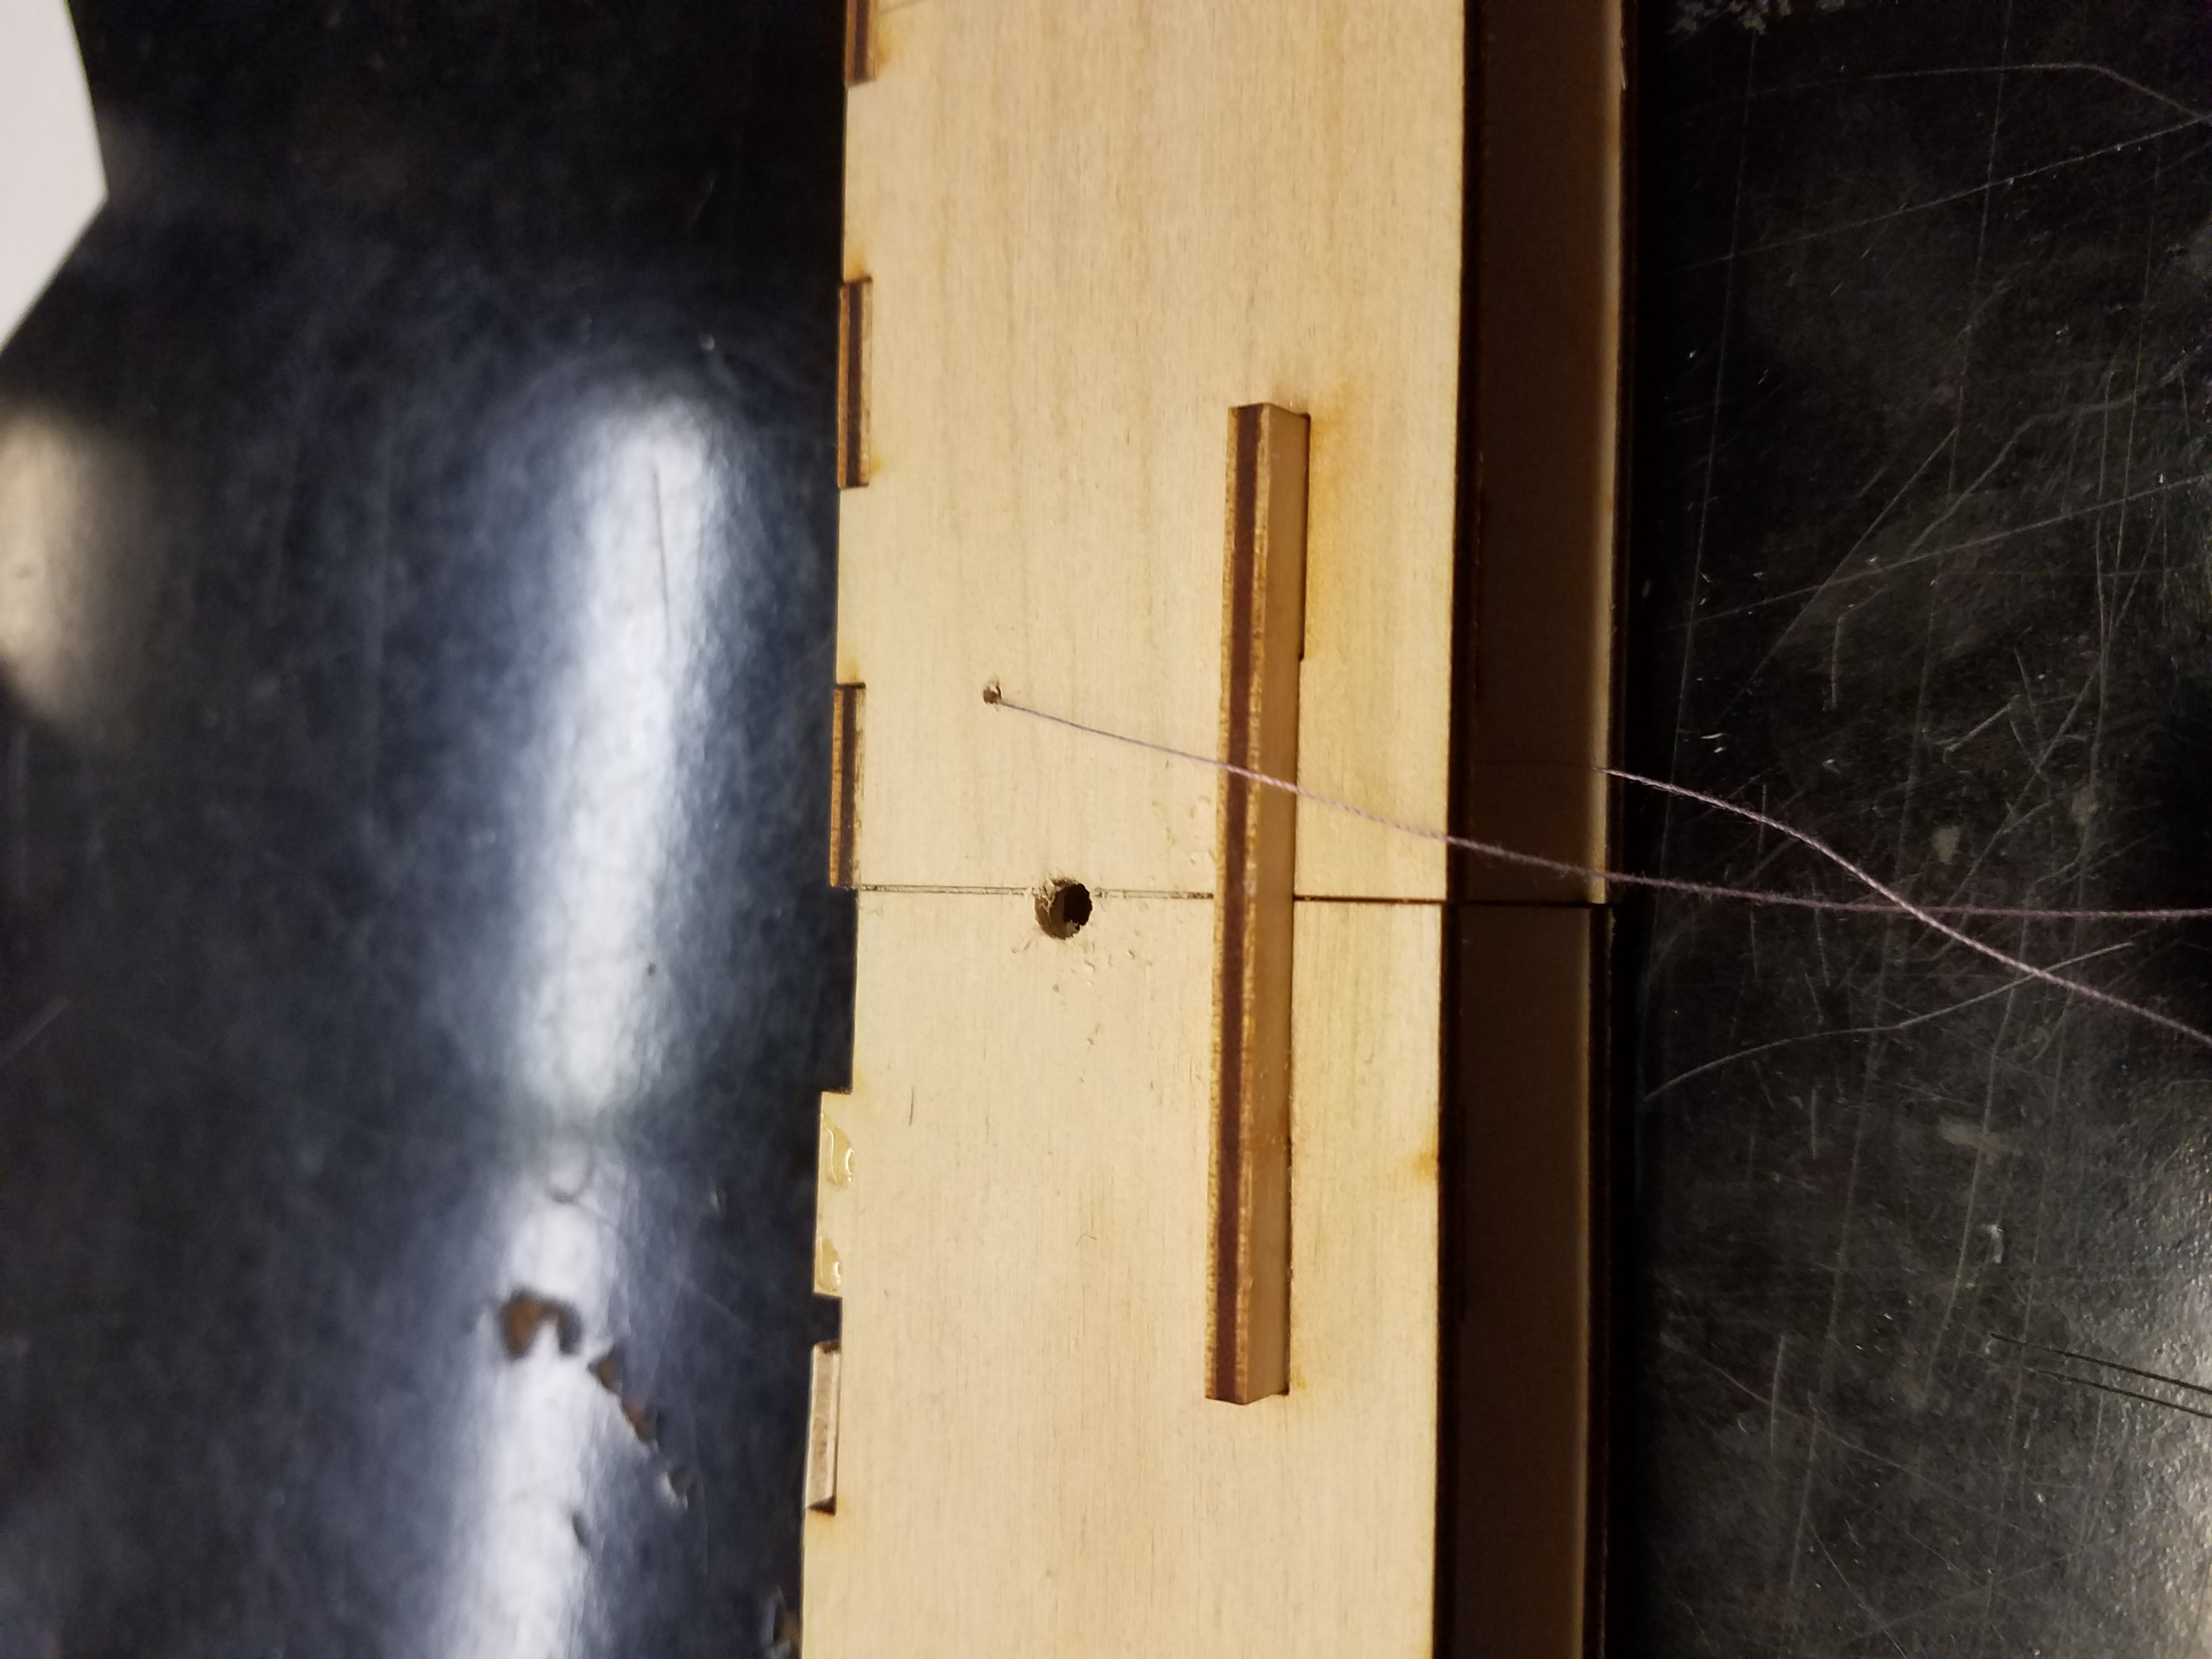
\includegraphics[width = 0.49\linewidth]{threading0.jpg}
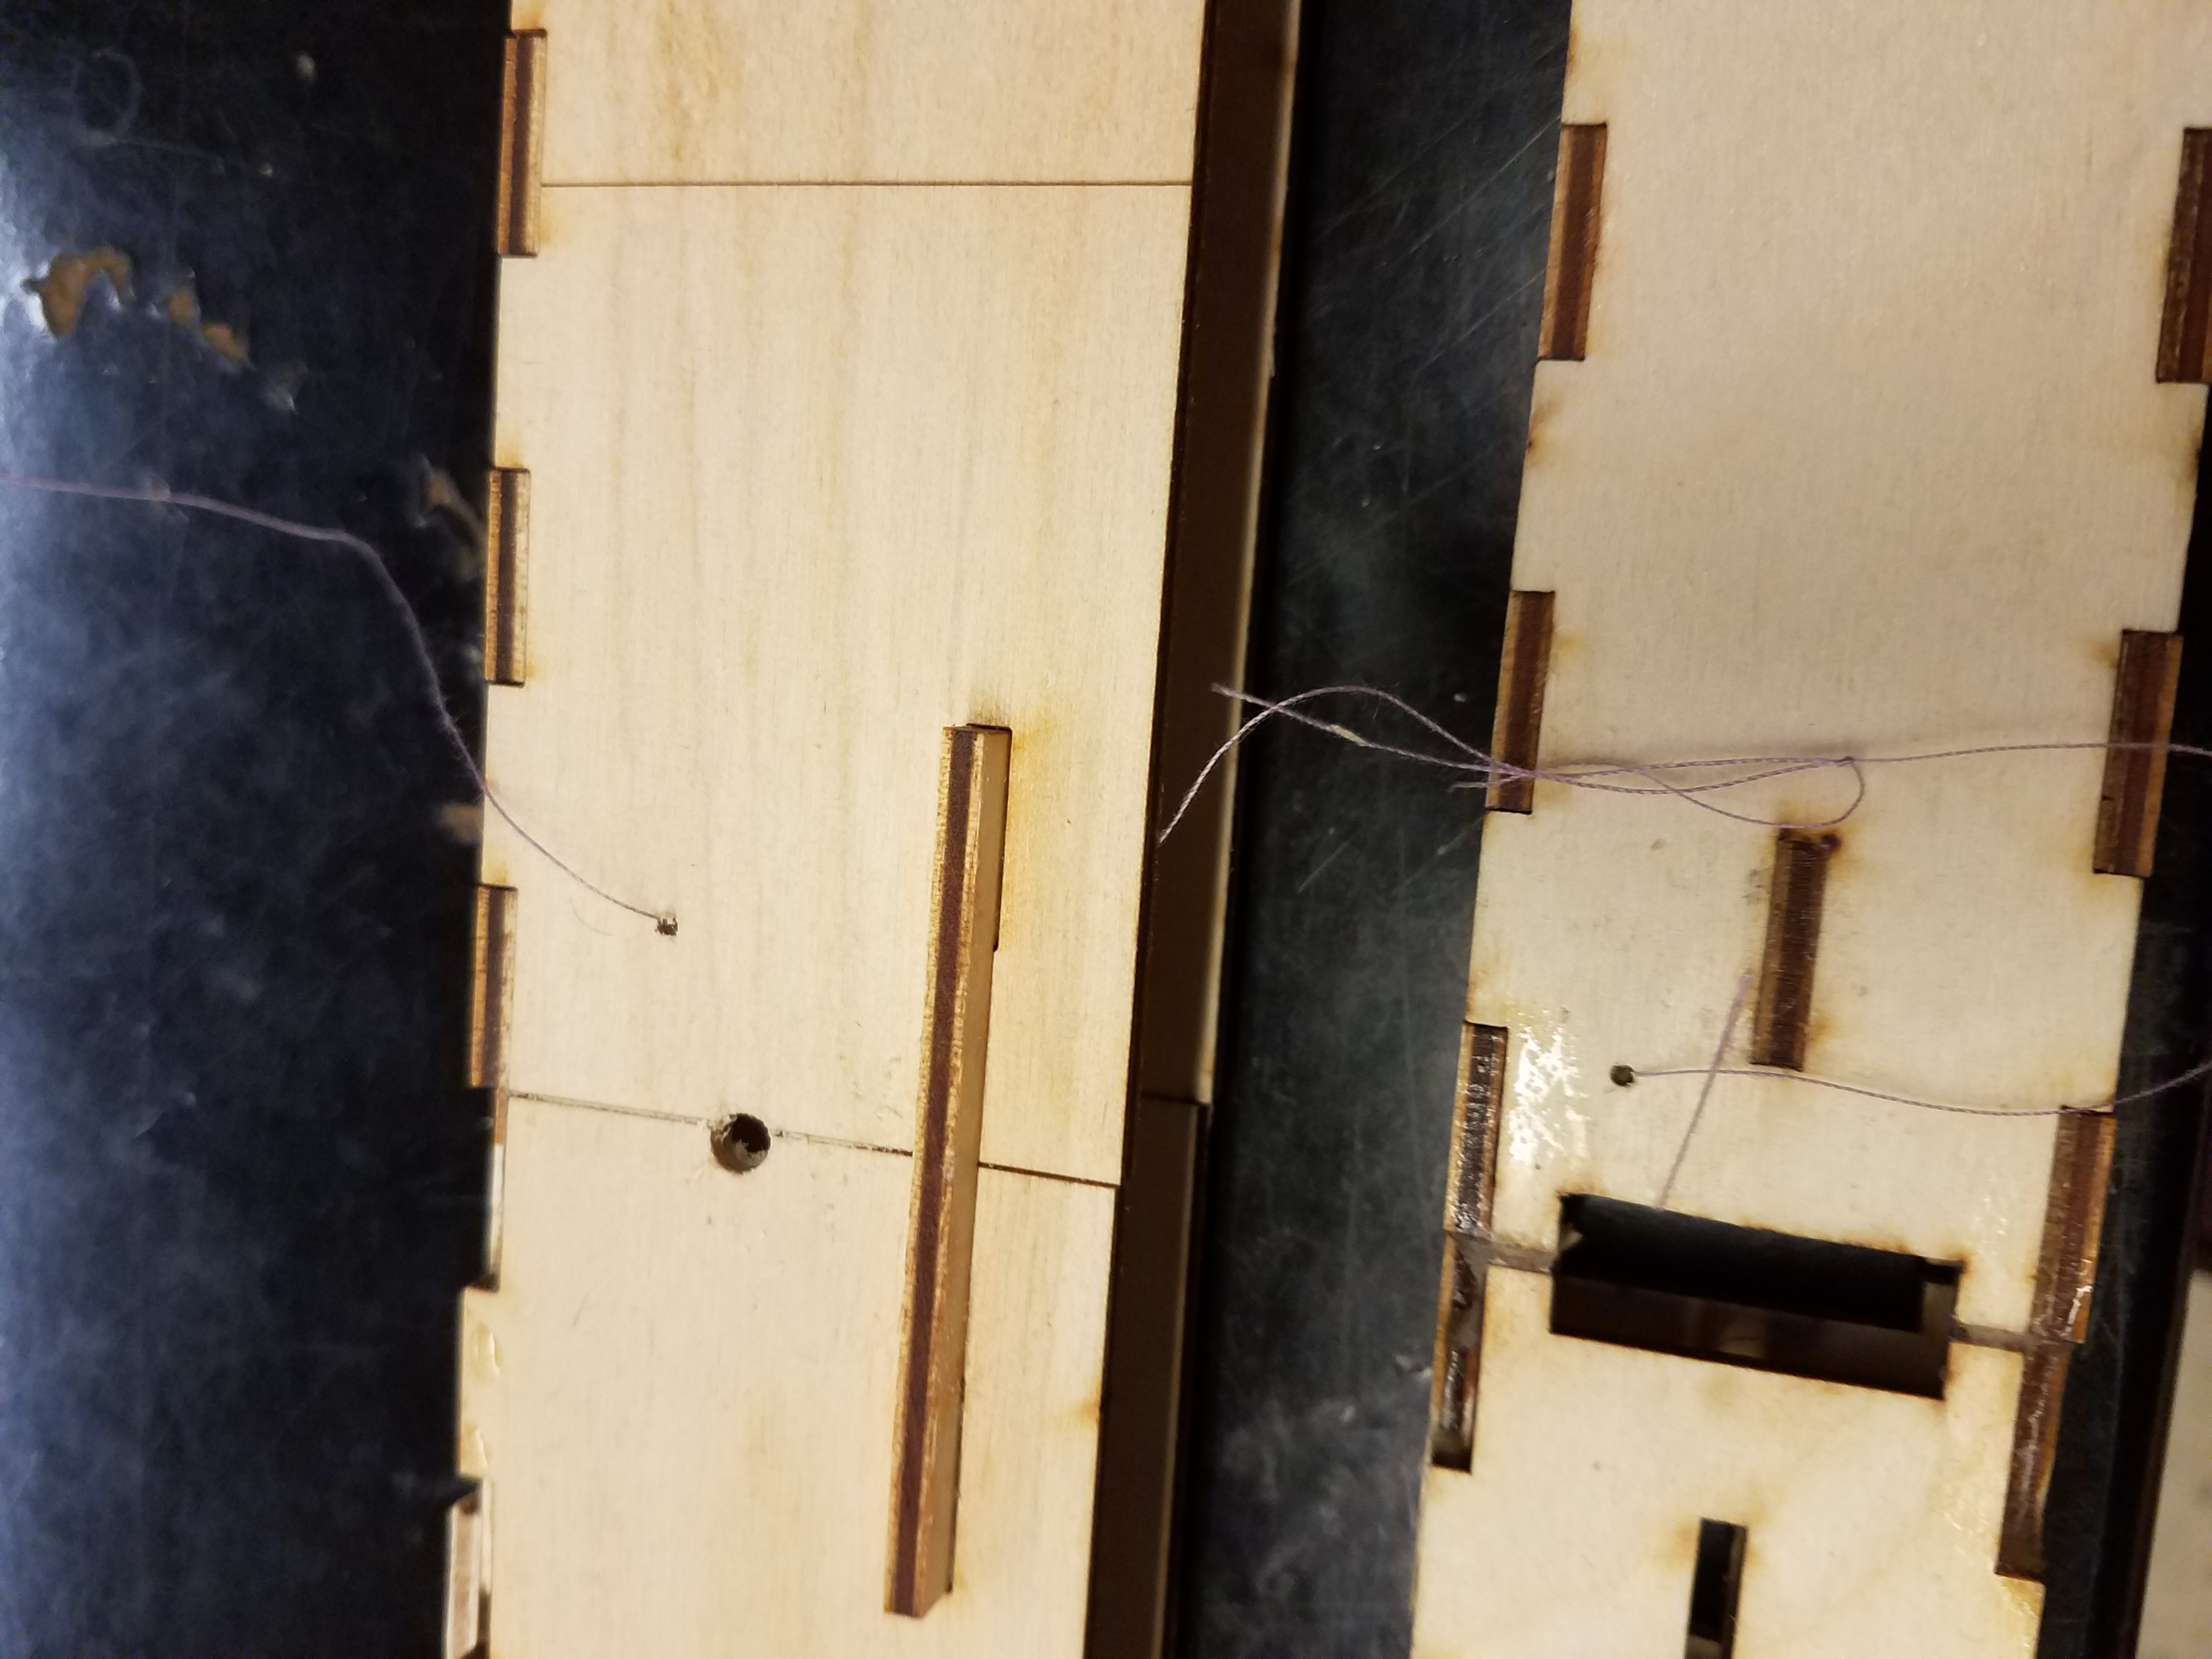
\includegraphics[width = 0.49\linewidth]{threading1.jpg}
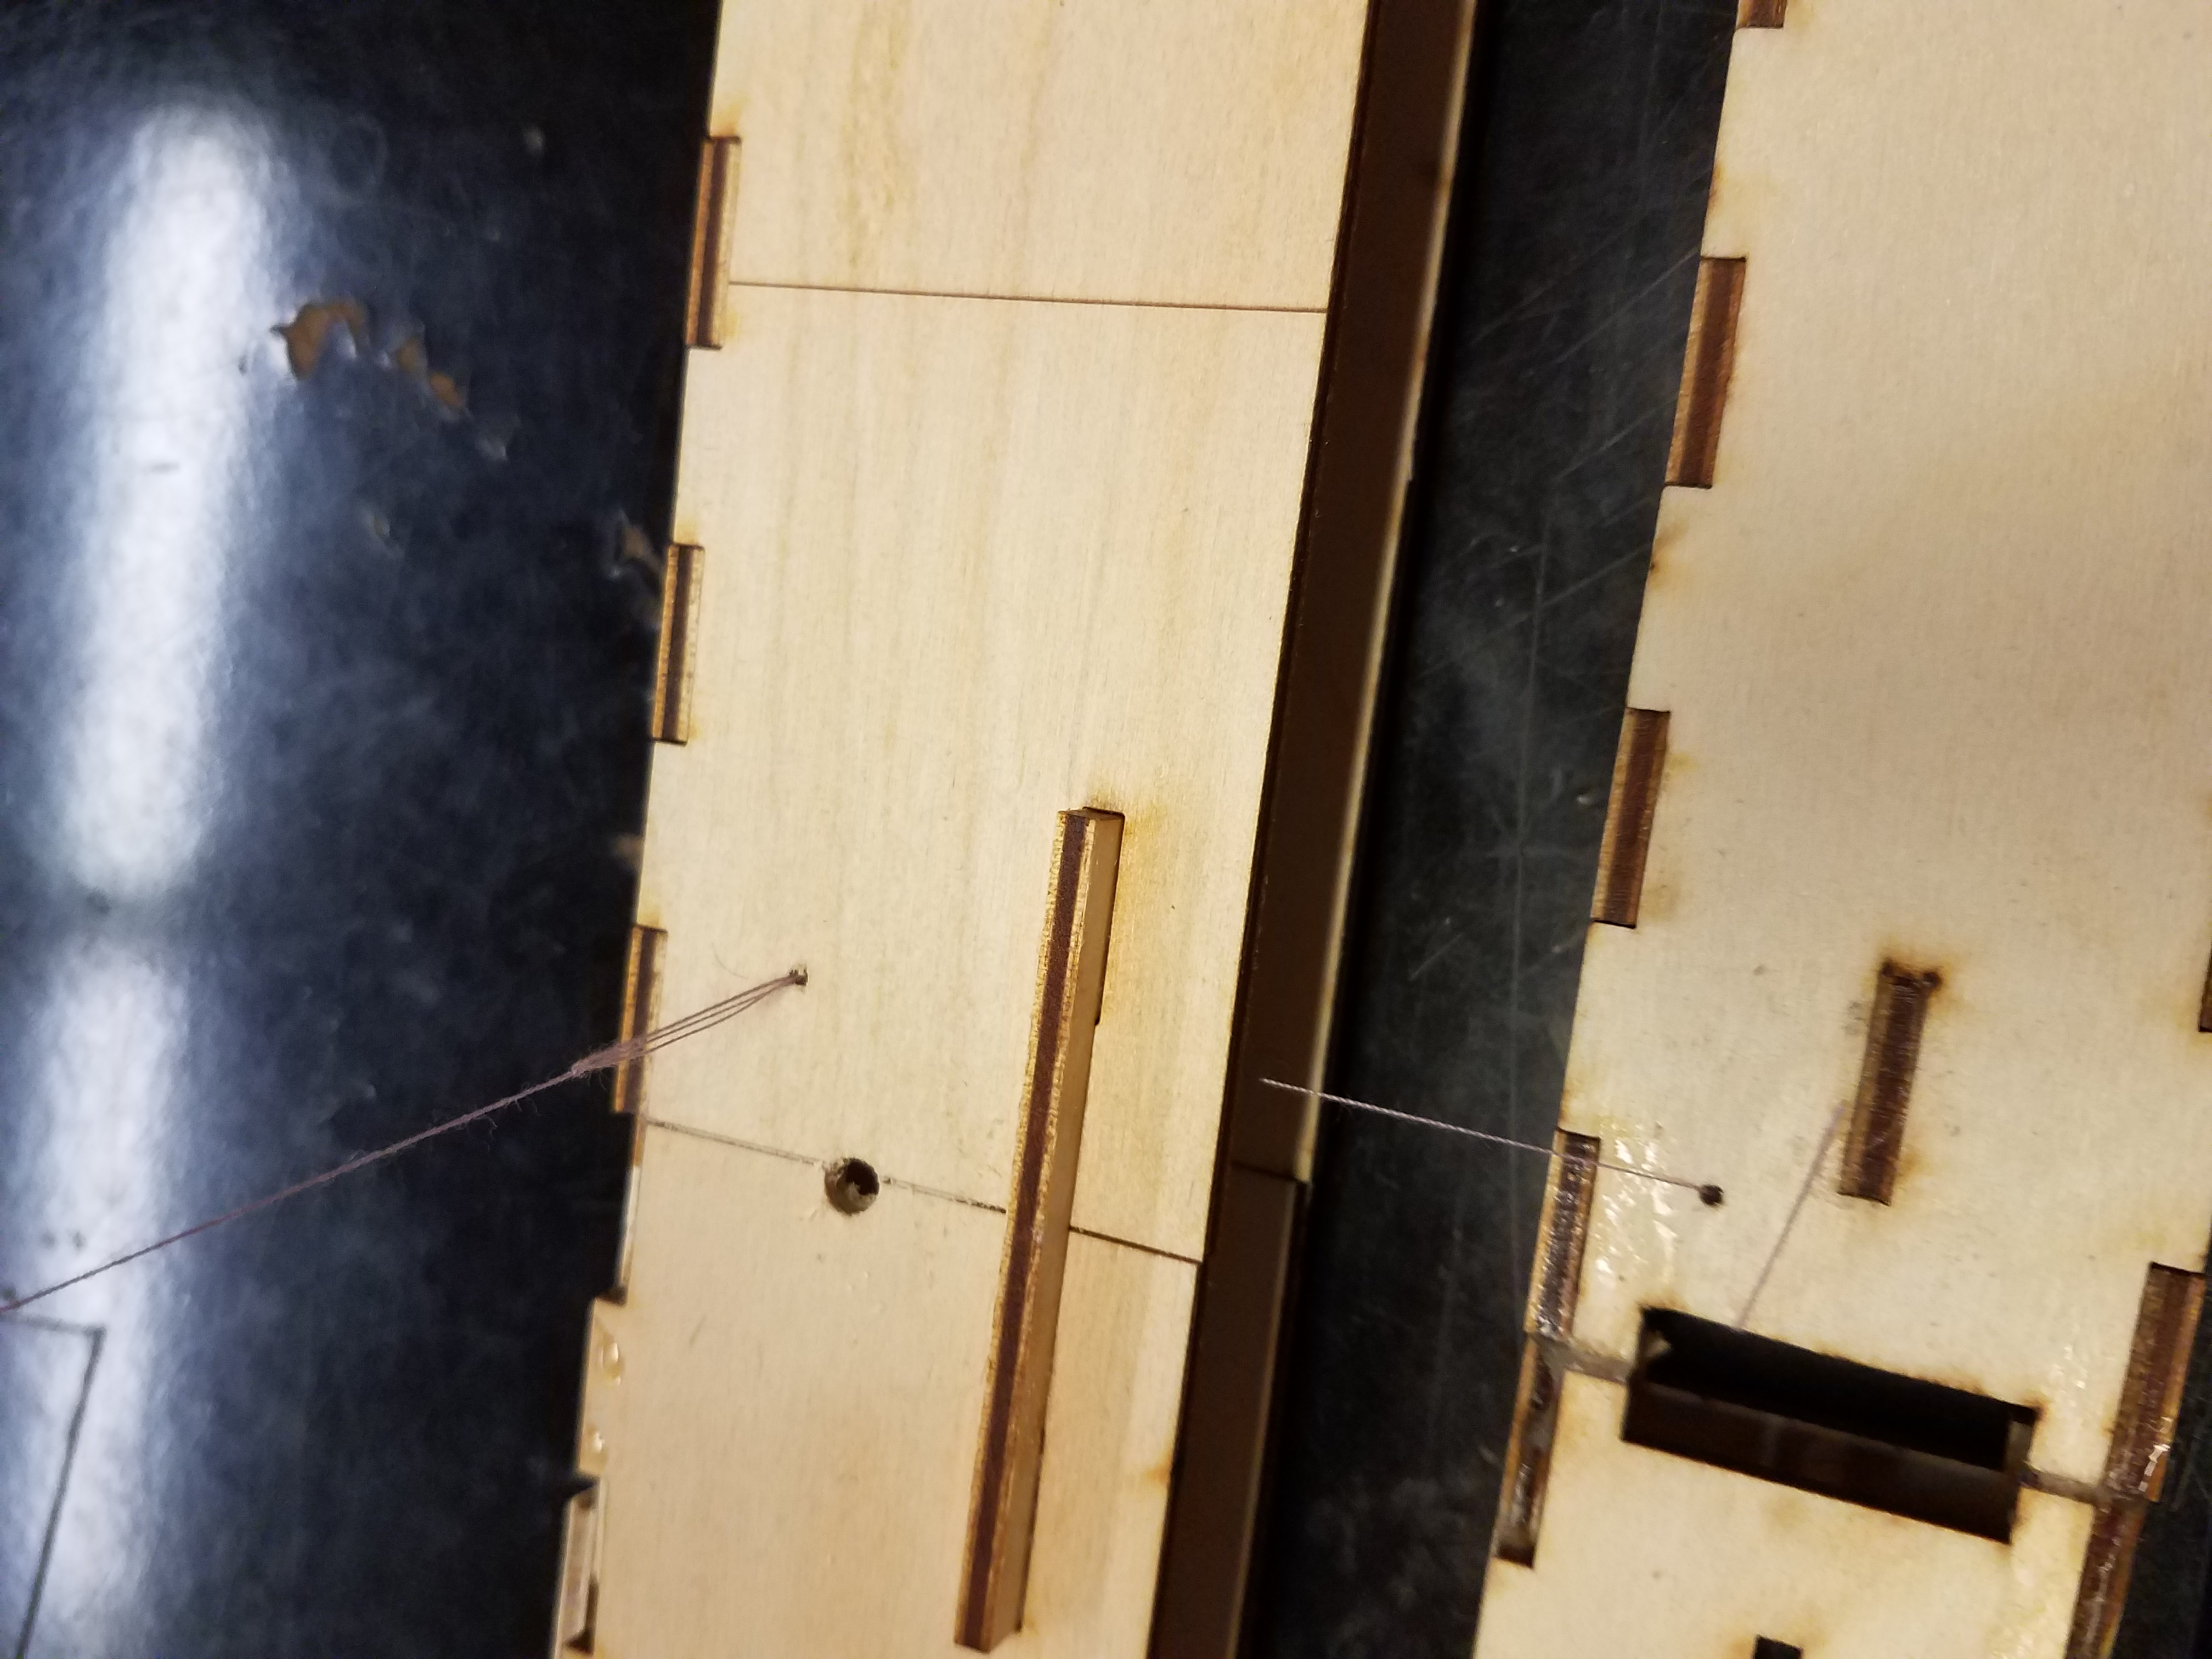
\includegraphics[width = 0.49\linewidth]{threading2.jpg}
\centering
\caption{The process of installing the threads from which the frame hangs.}
\label{thread_insertion}
\end{figure}

When the model is simply hanging, with no external force, the threads will generate no net horizontal force. However, in order
to determine their effect on the load cell measurements, we must consider what happens when there is a force on the model, and
the load cell deforms by a small amount. Theoretically, if the threads are perfectly vertical as intended, any horizontal force
they exert while be proportional to the square of the deformation, which should render it negligible. However, if some of the
threads are not perfectly vertical, then there may be a force which varies linearly with the deformation. In other words, it
will change the load cell measurement by a constant factor. Although this interferes with the measurement process, fortunately
it is easy to correct for. If the load cell measurements are calibrated by applying forces to the model with the load cell installed,
then any error due to the threads will be automatically corrected for implicitly in the calibration parameters.

Although the net error due to the threads can be easily corrected for, it has been realized that if the aerodynamic force on the
model is asymmetric, meaning there is a resultant moment about the vertical axis (which there should not be, if the model is
perfectly symmetric), then the model may twist to the side, which would cause the threads to exert a significant horizontal
force on it. Therefore, it is necessary to have some method of fixing the model's orientation. To this end, threads which
are not vertical but are slanted to the left and right (spanwise direction) where installed (Figure \ref{side_thread}). These
threads will prevent the model from rotating, but still exert no force in the streamwise direction (meaning that they will not
cause error in the drag measurement).

\begin{figure}
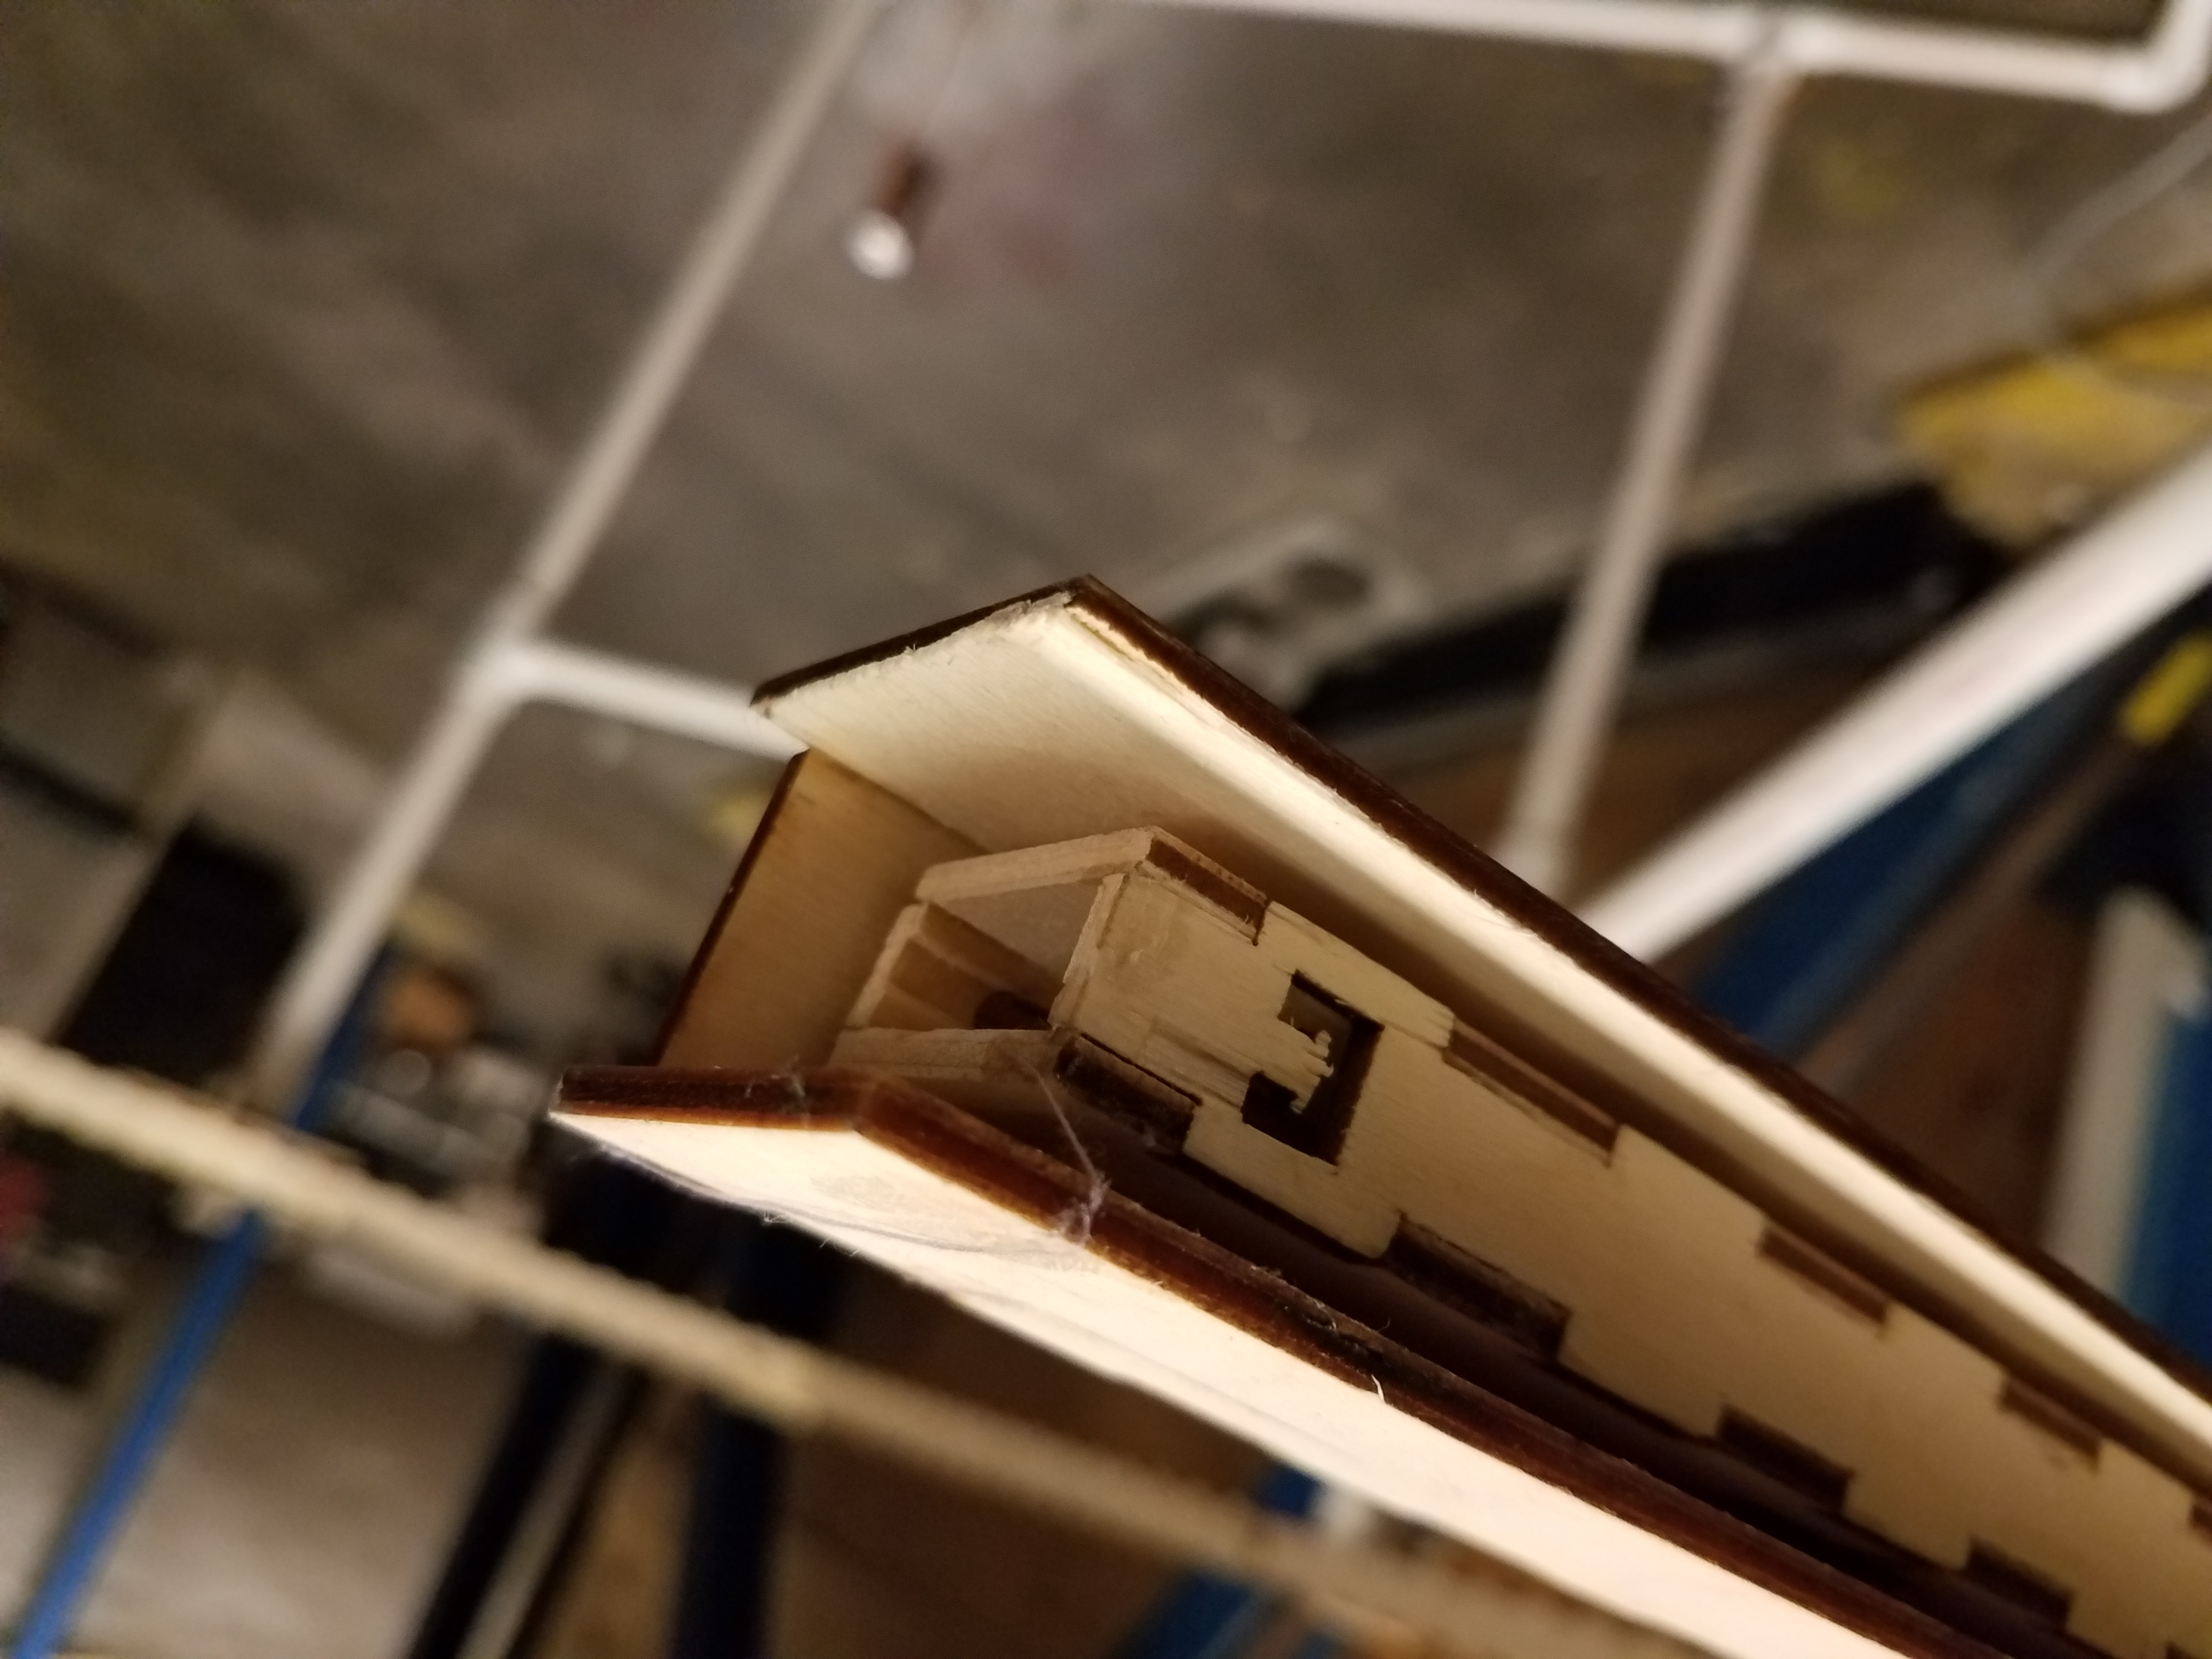
\includegraphics[angle=180,origin=c,width = 0.7\linewidth]{side_force.jpg}
\centering
\caption{Threads which are slanted in the spanwise direction prevent the frame from rotating inside the shell.}
\label{side_thread}
\end{figure}

The method of transfering load from the model to the load cell has been modified since the first iteration. Namely, instead
of placing the load cell in front of the rear member of the frame and tying it to the frame with a thread, it has been placed
behind the frame. A screw is driven into a nut which is attached to the frame, and the head of the screw pushes on the load
cell (see Figure \ref{load_transfer_screw}). This method has two advantages over the thread method. First, moving the load
cell behind the frame moves it away from the
model, which decreases the amount of aerodynamic interference. Second, the distance from the screw head to the model can be
easily adjusted, simply by turning the screw. Therefore, the screw can be adjusted so that when the model is hanging in equilibrium,
the screw barely touches the load cell, which is necessary in order to eliminate any error in the drag measurement caused by the
threads.

\begin{figure}
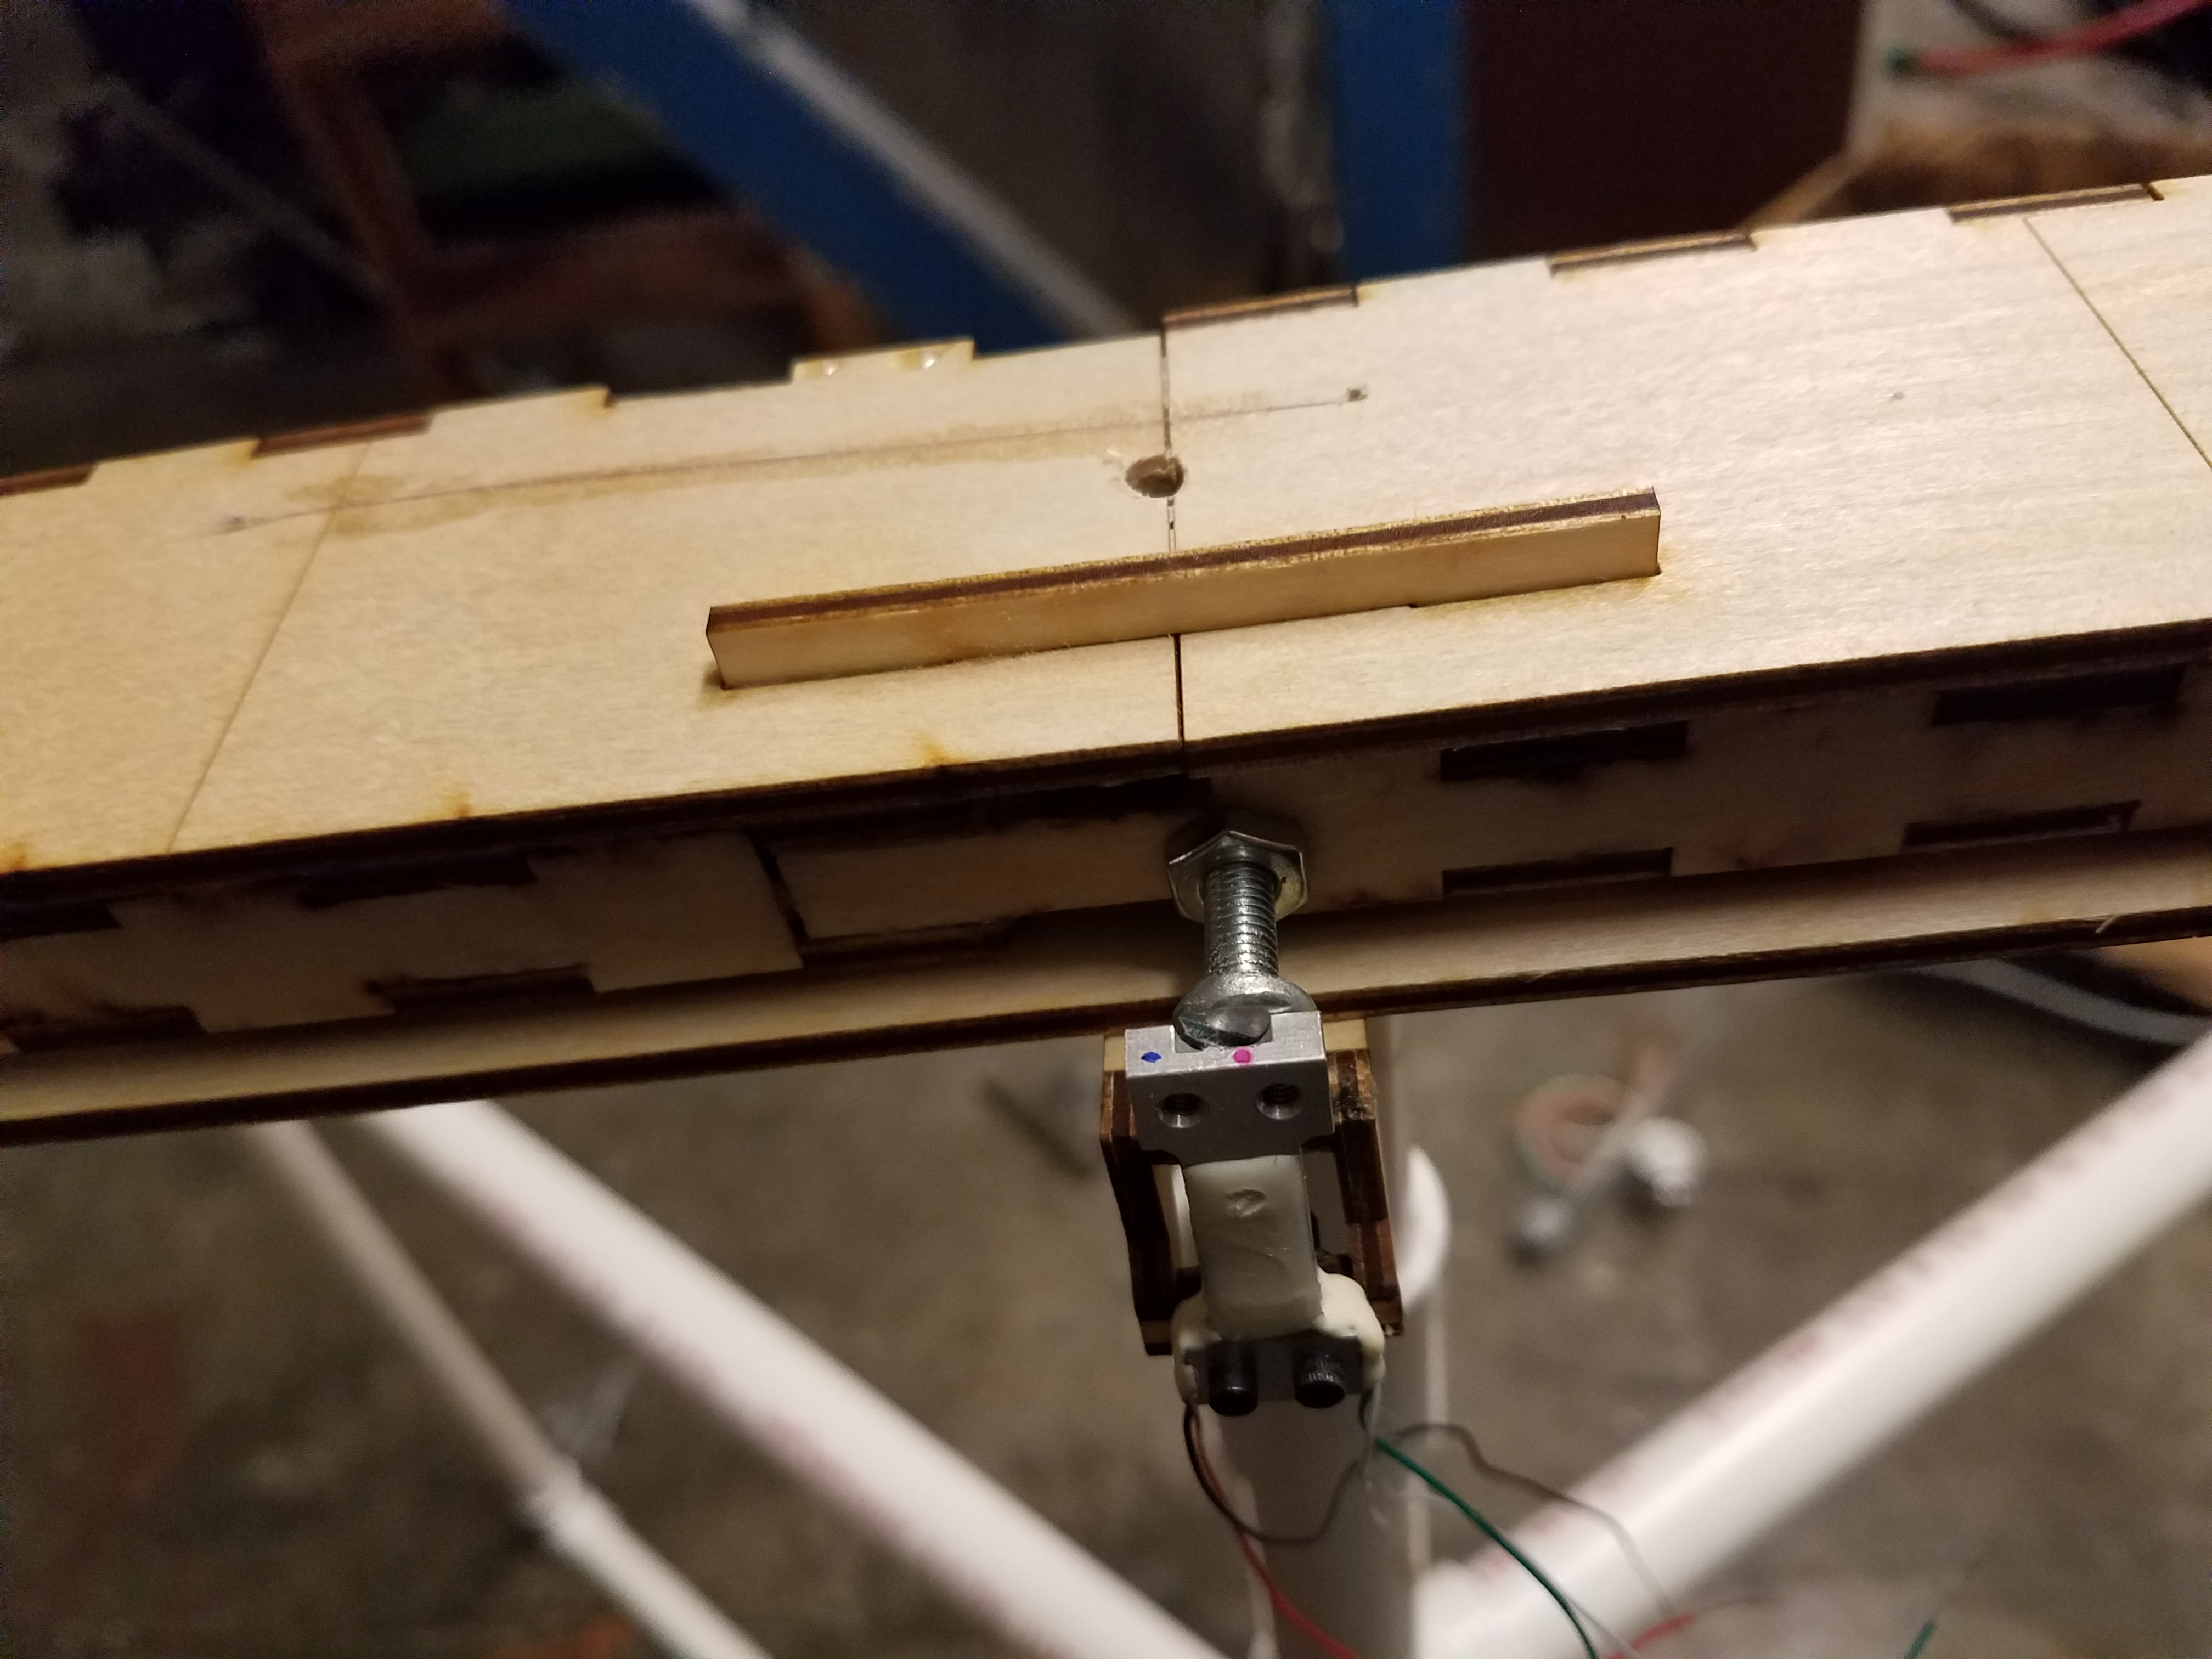
\includegraphics[width = 0.49\linewidth]{load_transfer_screw.jpg}
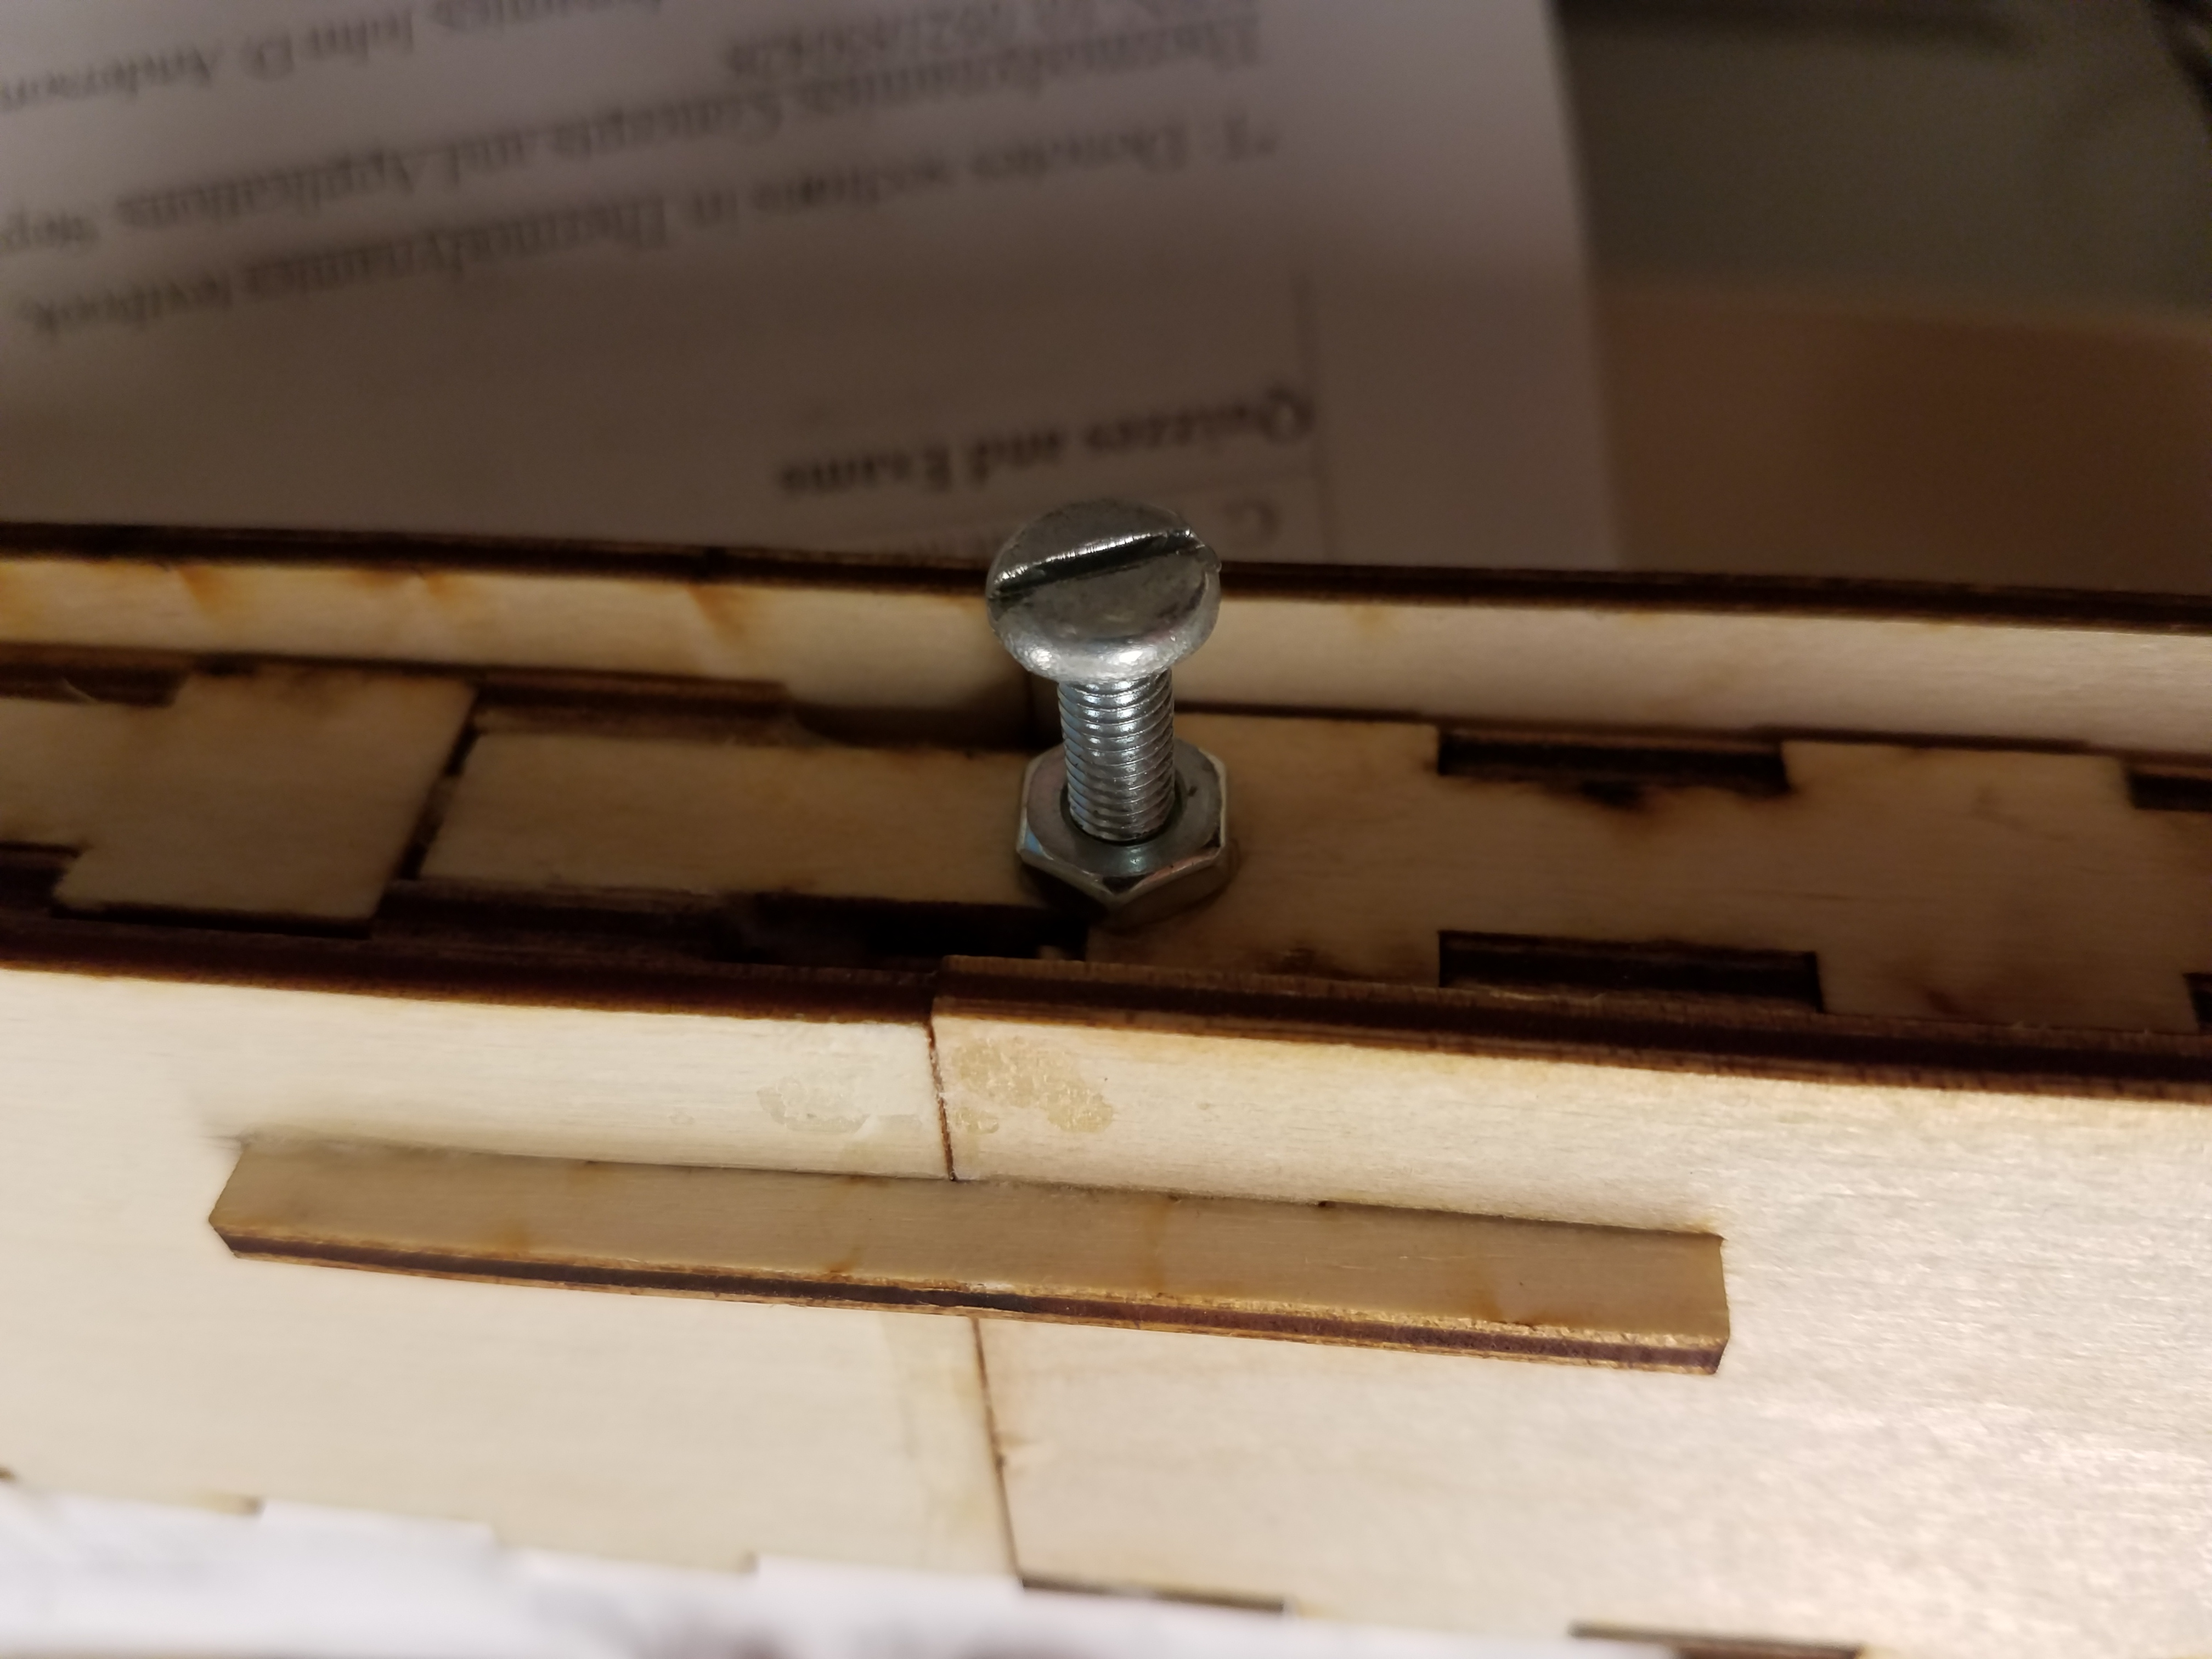
\includegraphics[angle=180,origin=c,width = 0.49\linewidth]{screw.jpg}
\centering
\caption{The screw which transfers the drag load from the model to the load cell.}
\label{load_transfer_screw}
\end{figure}

There was concern that the threads used to suppor the frame would affect the load cell measurements (which turned out to be justified).
So, a calibration trial was run with the second iteration. The same load cases were run as in the plain load cell calibration trial,
but instead of applying the load directly to the load cell, the loads were applied to the frame, as the drag loads would be. Because
the frame must be horizontal in order for the threads to operate properly, the loads could not simply be hung as before. Instead,
the weight was hung from a thread, an that thread was attached to two other threads. One thread extended upward at 45 degrees and was
attached to the wall, and another thread extended horizontally to the sheet frame. Basic statics can be used to show that the tension
in the horizontal thread is equal to the tension in the vertical thread (in a word, because the horizontal and vertical components
of the 45-degree thread are equal, and they must be canceled out by the tension in the horizontal and vertical thread, respectively).
Figure \ref{secondIterationCalibration} shows this setup. Note: If this procedure is repeated in the future, it is advisable to close
the doors to whatever room the test is being conducted in, to prevent ambient wind from causing the weights to swing).
A linear regression was fit to the readings (Figure \ref{secondIterationCalibrationPlot}), as described in Load Cell Calibration
and the conversion factor was found to be 2.24 N, which is roughly 1/6 of the value without the sheet in place. This is quite undesirable,
because it means our measurements are now 1/6 as sensitive due to the threads.

\begin{figure}
\includegraphics[width = 0.7\linewidth]{secondIterationCalibration.jpg}
\centering
\caption{The second iteration being calibrated in situ, to account for thread effects.}
\label{secondIterationCalibration}
\end{figure}

\section{Flow and Test Conditions}
The model was positioned in the test section, near the upstream end. It was positioned thus in order to be upstream of the apparatus
for the multirotor experiment. Figure \ref{positioning} shows the sheet frame in the wind tunnel, just before a test was run. To ensure
that precisely the component of the force which is parallel to the freestream is measured, a line perpendicular to the face of the load
cell was drawn on the rolling surface, and a string on the floor of the test section aligned with the streamwise structure of the wind
tunnel. The rolling surface was rotated so that the two lines were parallel (Figure \ref{roller_alignment}), and the roller bearings
of the sheet frame was made to roll
exactly along the line.

\begin{figure}
\includegraphics[width = 0.7\linewidth]{frame_in_tunnel.jpg}
\centering
\caption{The positioning of the model ahead of the other apparatus in the test section.}
\label{positioning}
\end{figure}

\begin{figure}
\includegraphics[width = 0.7\linewidth]{parallel_to_freestream.jpg}
\centering
\caption{Aligning the drag measurement to be parallel to the freestream.}
\label{roller_alignment}
\end{figure}

After running sufficient tests to ensure that the wind tunnel and measurement systems were under control, a two measurement tests
were run with only the sheet support structure. One was run at 5.0 m/s, and another at 6.9 m/s.

\chapter{Results and Discussion}
Drag measurements were obtained for the first-iteration frame at 5.0 m/s and 6.9 m/s. Table \ref{drag} displays the measurements.
The drag coefficients
were normalized based on the sheet's nominal area of $20 in \times 40 in$. The density was computed based on the ambient conditions in
the wind tunnel facility, $73\degree F$ and $30.5 inHg$. These were computed to density using the perfect gas equation of state.

Table \ref{drag}:
\begin{tabular}{c c c}
Flow speed [m/s] & Drag [N] & Drag Coefficient \\ \hline
5.0 & 0.769 & 0.0954 \\
6.9 & 1.37 & 0.0915 \\
\label{drag}
\end{tabular}

The drag of the frame is rather large compared to the predicted drag of the sheet. It does not appear to be prohibitively large, but
given the sensitivity of our measurements, which is not impressive, it will reduce our confidence in our final result. Perhaps after
the measurements have been taken, another support structure with even lower drag may be produced.

On a different note, although the drag fo the support structure does not exhibit a strong dependence on Reynolds number, so we are
fairly free to test at whatever Reynolds number we see fit (which will continue to be one which is as high as possible,
because a higher flow speed and chord increases the quantity of drag relative to the sensitivity of our measurement apparatus).

While the first-iteration frame was being tested, some flutter was observed. This flutter may cause the drag to vary which will reduce the precision
of our measurements. Furthermore, there is no guarantee that the average value of the drag would be the same with and without flutter.
Fortunately, however, when the wires which support the sheet were added, the flutter was reduced. Probably this was because the wires,
which were under tension, provided some additional support.

Figures \ref{data_example}, \ref{loadCellCalibration}, and \ref{secondIterationCalibrationPlot} display the data and regression fits for
the calibration trials. The regression fits are not nearly as close as would be hoped and expected, even when the weights were simply hung from
the load cell. It is possible that there were vibrations in the weight that could not be eliminated, or that there was a faulty wiring connection,
but it seems more likely that the load cells simply provide quite noisy data. So, no matter how much the mechanical sources of error can be reduced,
there will always be considerable random uncertainty due to the load cells.

Furthermore, the second iteration drag setup, which is expected to reduce the mount drag, in fact interfered with the mechanical force measurements.
It seems to simply change the calibration constant, but not affect the uncertainty of the data, so this should not be a serious problem. However,
it means that every time any aspect of the setup is changed, a new calibration trial must be conducted to take into account the effects of changes
to the structure.

Future work should attempt to find a way to suspend the frame which does not affect the measurements so severely.

\begin{figure}
\includegraphics[width = 0.7\linewidth]{data_example.jpg}
\centering
\caption{The raw data for the 2 oz calibration trial.}
\label{data_example}
\end{figure}

\begin{figure}
\includegraphics[width = 0.7\linewidth]{loadCellCalibration.jpg}
\centering
\caption{The averaged results for the calibration measurement.}
\label{loadCellCalibration}
\end{figure}

\begin{figure}
\includegraphics[width = 0.7\linewidth]{secondIterationCalibrationPlot.jpg}
\centering
\caption{The data from the Second Iteration calibration trial.}
\label{secondIterationCalibrationPlot}
\end{figure}

\chapter{Conclusions}

There were two aspects to this research: theoretical and experimental. The theoretical aspects were successful, although the experimental
aspects have not progressed far enough to validate the theoretical ones. As far as theory is concerned, a L/D target in order to fulfill
the glide requirement was established. In fact, a relationship between $C_L$ and $C_D$ which will fulfill the requirement was found, which
is shown in Figure \ref{requirements}. Furthermore, based on Fluent CFD, drag polars for the sheet were estimated. Also, the $C_D0$ for the
sheet was calculated analytically using Blasius' equation for laminar boundary layers. The CFD agreed with the Blasius solution for zero
angle of attack, as expected. Finally, the lift of the entire aircraft was estimated, taking into account the wing, the sheet, interaction effects,
and the sheet's lift curve slope (as estimated by CFD). However, unfortunately, these results have yet to be tested experimentally.

As far as experiment is concerned, the accomplishments this semester amount to developing techniques and equipment for taking measurements.
A method for measuring the drag of the sheet has been developed and the necessary apparatus constructed, but due repeated setbacks and
the need for precise calibration, it did not reach the point of actually testing the sheet. An axial force balance, an drag balance
for a sheet, and a model of the flying leaf all exist and are almost ready to test. In addition, there is a LabVIEW program for
recording and displaying drag readings. All that remains is to put everything in the wind tunnel and test it (with the necessary
calibration procedures). However, that is a time-consuming task, and may or may not be finished by the end of the semester.
Future work should begin with the methods that have been developed so far to conduct measurements and ideally improve the calibration
accuracy.

\begin{thebibliography}{6}

\bibitem{tradeoff}
Komerath, N., Shukla, D., Hariharan, S., Patel, S., et al., ``Tradeoff Study of High Altitude Solar Reflector Concepts,''
SAE Technical Paper 2017-01-2143, doi: 10.4271/2017-01-2143

\bibitem{flyingCarpet}
Komerath, N., Hariharan, S., Shukla, D., Patel, S., et al., ``The Flying Carpet: Aerodynamic High-Altitude Solar Reflector Design Study,''
SAE Technical Paper 2017-01-2026, 2017, doi: 10.4271/2017-01-2026

\bibitem{us}
Micaiah C. Smith-Pierce, Yana Charoenboonvivat, Dhwanil Shukla, and Narayanan M. Komerath. ``High Altitude Aerodynamic Reflectors To
Counter Climate Change'', 2018 Applied Aerodynamics Conference, AIAA AVIATION Forum, (AIAA 2018-3963)
\verb|https://doi.org/10.2514/6.2018-3962|

\bibitem{Anderson}
John Anderson, \textit{Fundamentals of Aerodynamics}, 6th edition

\bibitem{standardAtmosphere}
Standard Atmosphere calculator
\verb|https://www.digitaldutch.com/atmoscalc/index.htm|

\bibitem{AVL}
Mark Drela, Harold Youngren, Athena Vortex Lattice
\verb|http://web.mit.edu/drela/Public/web/avl/|

\end{thebibliography}

\end{document}
